%%
%%%%%%%%%%%%%%%%%%%%%%% file typeinst.tex %%%%%%%%%%%%%%%%%%%%%%%%%
%
% This is the LaTeX source for the instructions to authors using
% the LaTeX document class 'llncs.cls' for contributions to
% the Lecture Notes in Computer Sciences series.
% http://www.springer.com/lncs       Springer Heidelberg 2006/05/04
%%
% It may be used as a template for your own input - copy it
% to a new file with a new name and use it as the basis
% for your article.
%
% NB: the document class 'llncs' has its own and detailed documentation, see
% ftp://ftp.springer.de/data/pubftp/pub/tex/latex/llncs/latex2e/llncsdoc.pdf
%
%%%%%%%%%%%%%%%%%%%%%%%%%%%%%%%%%%%%%%%%%%%%%%%%%%%%%%%%%%%%%%%%%%%


\documentclass[runningheads,a4paper]{llncs}

\usepackage{amssymb}
\usepackage{apacite}
\usepackage{caption}
\usepackage{multirow}
\usepackage{bm}
\usepackage{siunitx}
\usepackage{xfrac}
\usepackage{enumitem}
%\usepackage{subcaption}   % To make subfigures. Read subfigure.pdf on ctan.tug.org
\usepackage{feynmp}
\DeclareGraphicsRule{*}{mps}{*}{}

\usepackage{graphicx}
\usepackage{cancel}
\usepackage[intlimits]{amsmath} % Puts the limits of integrals on top and bottom
\usepackage{amsxtra}     % Use various AMS packages
%\usepackage{amsthm}
\usepackage{amssymb}
\usepackage{subfigure}
\usepackage{amsfonts}
\usepackage{graphicx}    % Add some packages for figures. Read epslatex.pdf on ctan.tug.org
\usepackage{rotating}
\usepackage{color}
\usepackage{epsfig}
%\usepackage{subcaption}   % To make subfigures. Read subfigure.pdf on ctan.tug.org
\usepackage{float}

\setlength{\parfillskip}{0pt}

\newcommand{\sun}{\ensuremath{\odot}} % sun symbol is \sun
\newcommand{\metrel}{$E_{\text T}^{\text {miss,rel}}$}
\newcommand{\dileptonmass}{$m_{\ell \ell}$}
\newcommand{\mttwo}{$m_{\text{T2}}$}
\newcommand{\invfb}{fb\textsuperscript{-1}}
\newcommand{\lumi}{$\int \mathcal{L} \, \mathrm{dt}$}
\newcommand{\met}{$E_{\text T}^{\text {miss}}$}

\usepackage{url} 
\newcommand{\keywords}[1]{\par\addvspace\baselineskip
\noindent\keywordname\enspace\ignorespaces#1}

\begin{document}

\mainmatter  % start of an individual contribution

% first the title is needed
\title{LHC Data Challenge\\Establishing a Bound on the Higgs and Z' Boson Mass}

% a short form should be given in case it is too long for the running head
\titlerunning{Establishing a Bound on the Higgs and Z' Boson Mass}

% the name(s) of the author(s) follow(s) next
%
% NB: Chinese authors should write their first names(s) in front of
% their surnames. This ensures that the names appear correctly in
% the running heads and the author index.
%
\author{Adam Garay Jalloh%
%\thanks{Please note that the LNCS Editorial assumes that all authors have used
%the western naming convention, with given names preceding surnames. This determines
%the structure of the names in the running heads and the author index.}%
\and Dhruva Gowda Storz\and Mark Fingerhuth\and Samuel Natarajan\and\ Henry Rice\and Annabel Wolf}
%
\authorrunning{LHC Data Challenge}
% (feature abused for this document to repeat the title also on left hand pages)

% the affiliations are given next; don't give your e-mail address
% unless you accept that it will be published
\institute{Maastricht Science Programme, Maastricht University,\\
Maastricht, The Netherlands\\
}

%
% NB: a more complex sample for affiliations and the mapping to the
% corresponding authors can be found in the file "llncs.dem"
% (search for the string "\mainmatter" where a contribution starts).
% "llncs.dem" accompanies the document class "llncs.cls".
%

\toctitle{Lecture Notes in Computer Science}
\tocauthor{Authors' Instructions}
\maketitle


\begin{abstract}
A collection of 1 $\invfb$ of ATLAS data from measurements taken in 2012 are used to establish a bound on the mass of the Higgs boson and Z'. Background processes are examined and suppressed to identify the target signal processes. According to the performed analysis a total of \lumi = 50.5 $\invfb$ is required for a statistically significant difference of 5 $\sigma$ for the Higgs and \lumi = 34 $\invfb$ is required for the Z'. Monte-Carlo simulations provide indication of the accuracy of the analysis.\\

\keywords{Higgs boson, Z' boson, Particle physics, Standard Model}
\end{abstract}
\vspace{12mm}
%%SAM & AN START
\section{Introduction}
A major hallmark of modern physics is the Standard Model (SM), a quantum-field theory, which is currently the most complete explanation of the elementary foundations of the known universe. The ATLAS experiment at CERN is aimed at understanding and explaining the shortcomings of the Standard Model; how mass is created due to the Higgs field, the reason for the missing anti-matter in the universe, and the nature of dark matter and dark energy. To solve these mysteries ATLAS must push the boundaries of established ideas and search for new physics in the high energy realm. Scaling up the maximum energy of the LHC to 13 TeV now motivates searches for beyond-the-Standard-Model (BSM) scenarios, of which supersymmetry is a popular candidate as it may be able to unify the four fundamental forces by including gravity in the SM.\\

This report discusses data collected from the ATLAS detector in 2012 which was released publicly in June 2016. An overview of the most important background processes in new physics searches will be provided as well as an explanation for how a signal can be distinguished from the background. Additionally, the statistical analysis of the Higgs and Z' boson search is discussed.\\

\subsection{The LHC and ATLAS}
The Large Hadron Collider, located at CERN, Geneva, is the largest and most powerful particle accelerator in the world. It consists of a ring, about 27 kilometres in circumference, with a number of accelerating structures to accelerate the particles close to the speed of light. Within the loop there are two beam pipes surrounded by superconducting magnets which accelerate the charged particles in opposite directions around the ring. The LHC is used by an international team of scientists to investigate and probe the fundamental nature of the universe.\\

ATLAS, A Toroidal LHC Apparatus, is one of the four main particle detectors located along the LHC where proton collision experiments are conducted amongst others. Two high-energy particle beams, each with 2808 bunches of ${10}^{11}$ protons, travel through the accelerator close to the speed of light in an ultrahigh vacuum (${10}^{–13}$ atm) and at a temperature of $-271.3$ \textdegree C in opposite directions \cite{CERN}. The two beams are aligned to collide inside the ATLAS detector, which uses a large array of detectors organised in cylindrical shells to measure the properties of the particles produced in proton beam collisions.\\

Each layer of the detector is designed to reconstruct as much information about the particles as possible. The first layer consists of tracking devices, which measure the path of electrically charged particles by analysing the signals that they create from ionizing the matter in the device \cite{aad2012observation}. A large, toroidal, superconducting magnet creates a complex magnetic field that alters the trajectory of the charged particles through this first layer. This allows for the particle’s momentum to be determined by measuring the curvature of the non-linear trajectory. Tracking devices either consist of a gaseous chamber or a semiconductor detector. In gaseous chambers, electrons or ions are collected on electrodes under a strong electric field, whereas semiconductor detectors measure the voltage generated by electron-hole pairs that appear when the charged particles pass through a reverse-biased semiconductor \cite{aad2012observation}. The next layer of the detector is an electromagnetic calorimeter. This absorbs all electrons and photons, which have electromagnetic properties. Hadrons begin to lose energy in this stage, but are not stopped until they reach the hadronic calorimeter. The final layer of the detector identifies and measures muons. Fig. \ref{fig:atlas} provides a schematic overview of the ATLAS detector.\\
\begin{figure}
\centering
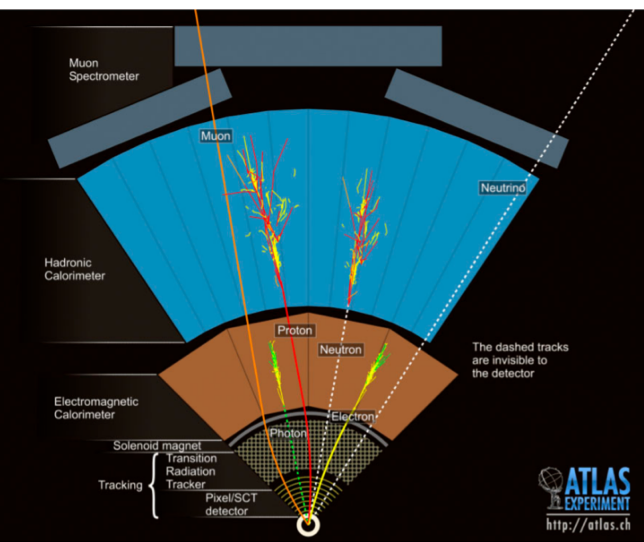
\includegraphics[height=7cm]{atlas}
\caption{Overview of the different layer of the ATLAS detector. Retrieved from:
http://atlas-opendata.web.cern.ch/atlas-opendata/webanalysis/}
\label{fig:atlas}
\end{figure}
\pagebreak
\subsection{The Standard Model}

The SM is a rigorously tested mathematical model that describes the properties and interactions of elementary particles. It is a quantum field theory, which reconciles quantum mechanics and the relativistic effects experienced by the elementary particles at high energies. Quantum field theory interprets elementary particles as excited states of their corresponding physical fields, known as field quanta. The SM is composed of three generations, often referred to as flavour, of quarks and leptons, four gauge bosons and the Higgs boson (see Fig. \ref{fig:standardmodel}). The formulation of the mathematical equaton used to make calculations for the SM is known as the Lagrangian. The SM has resulted in the prediction and subsequent discovery of the Higgs Boson; the mode of interaction between energy and space-time, which gives mass to particles that interact with it.\\

%CITATION!
\begin{figure}
\centering
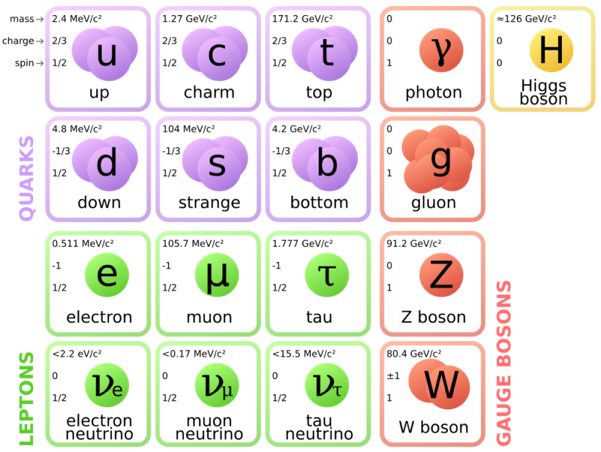
\includegraphics[height=6.5cm]{standardmodel}
\caption{The elementary particles described by the SM. Retrieved from: https://en.wikipedia.org/wiki/Standard\_Model}
\label{fig:standardmodel}
\end{figure}

\vspace{10mm}
As mentioned previously, every elementary particle can be said to have a corresponding field residing within space-time. The motion of particles can be described by ripples in their respective fields. Each of these fields is considered to be a quantum mechanical operator that has the ability to create particles out of the ground-state or vacuum. Therefore, it is possible to violate the law of conservation of energy for short periods of time due to the energy-time uncertainty relation. The creation of particles is comparable to ripples in the field that move through space-time \cite{raby1997neutrino}. The four fundamental forces (electromagnetic, strong, weak, and gravitational) are mediated by the exchange of virtual gauge bosons, with the exception of gravity whose force mediator remains unclear to this day.\\

The up and down quarks, along with the electron and electron neutrino make up the first generation of particles and are the lightest and most stable. All stable matter in the universe consists of first generation particles. Second and third generations are less stable and heavier. Quarks come in different colours and only mix with each other to form colourless combinations. Leptons consist of electrons, muons and taus, which are electrically charged and have mass; and their conjugate neutrinos, which are neutral and have very little mass.\\

Weak, electromagnetic and strong forces result from the exchange of force-carrier particles, which are all bosons. The strong force is carried by the gluons, the electromagnetic force by the photon and the weak force by ${W}^{+}$,${W}^{-}$ and Z bosons.\\

The Higgs boson is one of the most recent discoveries in the field of particle physics and it has been postulated that its interaction with the Higgs field creates a “friction” on the particle. This friction limits the particle’s energy so that it can no longer travel at the speed of light, and consequently acquires mass  \cite{melnikov2010w+}.\\

\pagebreak
\subsection{Collision Dynamics}

Protons are hadrons that are composed of quarks and gluons which may interact at the point of collision and form new particles. The particles of interest, which scientists intend to study, are usually present directly after the collisions. These particles then decay into other particles (usually more stable ones with lighter mass) through the mediation of bosons. All these processes can be best described with Feynman diagrams.\\

Importantly, charge and momentum are conserved during the decay process, allowing us to extract the invariant mass of the original particle. The decay process can happen several times before anything is measured in the detector. Furthermore, several decay processes can produce the same stable particles. Considering these factors, it is difficult to isolate the target decay process since vast amounts of events are happening in each proton bunch. In this sense there is a considerable quantity of background "noise" which must be suppressed to correctly identify processes of interest.

\subsection{Mathematical Concepts}

%% DHRUVA START
As the LHC accelerates particles close to the speed of light, it leaves the territory of classical dynamics and enters that of relativity. This also manifests mathematically and it becomes necessary to use a relativistic framework to describe the events. One of the most elementary changes brought about by this change is the use of 4-vectors instead of 3-vectors \cite{griffithsintroduction}. 4-vectors differ from 3-vectors only in an extra ${0}^{th}$ component, which usually involves a time dependent factor as the concept of absolute time does not exist in relativity. This extra component provides a large number of tools that simplify relativistic mathematics. A prime example is the Lorentz transformation tensor, which can be used to easily transform 4-vectors between inertial frames.\\

The most useful 4-vector for the intents of the analyses in this paper is the momentum 4-vector. With ${E}/{c}$ as the ${0}^{th}$ component, conserving 4-momentum automatically translates to energy and momentum conservation. Considering that mass, energy and momentum are tied together by Einstein's mass-energy equation (Eq. 1), this simplification is of great use as it is possible to reconstruct collision events using 4-momentum conservation. \\

\begin{equation}
{ E }^{ 2 }\quad ={ \quad (pc) }^{ 2 }\quad +\quad { (m{ c }^{ 2 }) }^{ 2 }
\end{equation}

The first and most essential piece of information obtained in the detectors is the transverse 4-momenta of all the particles identified in the collision event. Transverse 4-momentum is the momentum in the xy-plane with the beam traveling in the z-direction. Since none of the collision products travel exclusively in the z-direction, the sum of transverse momenta of all the decay products add up to the initial momentum of the beam. Therefore, in conjunction with a few other necessary measurements, a variety of conclusive data can be calculated from 4-momentum such as invariant mass, missing transverse energy (relevant when undetectable particles are produced) and reconstructed transverse mass. \\

A lot of information can be derived from the mass of a particle. However, ordinary mass cannot be used at velocities approaching the speed of light as it does not remain constant in different inertial frames. The invariant or relativistic mass is introduced to circumvent this problem as it is defined as the mass of a body at rest \cite{helliwell2010special}. The mass in a certain inertial frame can then be calculated by transforming the rest mass with the relativistic factor of $\gamma$ defined in Helliwell (2010):\\

\begin{equation}
\gamma \quad =\quad \frac { 1 }{ \sqrt { 1-\sfrac { { v }^{ 2 } }{ { c }^{ 2 } }  }  } 
\end{equation}

Invariant mass is useful in LHC detectors as the invariant mass of a decaying particle can be found by calculating it from the 4-momentum vector of the decay products. This is an essential process as the actual decay mechanism cannot be directly detected, but must be inferred from the products. The energy-time uncertainty relation enables particles to be heavier or lighter than their true mass which is known as off-shell particles. Due to this phenomenon, the invariant mass of the decaying particle is not always found to be the true mass of the particle in question, but manifests itself instead as a probability distribution centered around the true mass of the decaying particle. The peak of the invariant mass histogram therefore represents the true invariant mass of the particle being investigated.\\

Often, one encounters a case where the transverse momenta of the fragments do not add up to that of the colliding particles. This phenomenon can be due to the production of particles such as neutrinos that cannot be detected by the detectors. To solve this problem, the 4-momentum vector required to balance the initial and final 4-momenta is calculated. This vector is called the missing transverse energy ($\cancel{\it{E}}_{T}$). $\cancel{\it{E}}_{T}$ is useful in reconstructing events such as W decays in which an undetectable neutrino is produced. By calculating exactly how much energy is missing in the collision, it is possible to calculate the 4-momentum of the neutrino that was produced. This can then be used to reconstruct information about the decaying particle, such as the reconstructed transverse mass (${m}_{T}$). The ${m}_{T}$ of a W boson can be calculated using Eq. 3 \cite{aaltonen2012precise}.\\

\begin{equation}
{ m }_{ T }\quad =\quad \sqrt { 2{ p }_{ T }^{ l }{ p }_{ T }^{ v }(1-cos\Delta { \phi  }_{ lv }) }
\end{equation}
 
where ${ p }_{ T }^{ l }$ represents the transverse momentum of the lepton, ${ p }_{ T }^{ v }$ represents the transverse momentum of the neutrino (which is assumed to be the $\cancel{\it{E}}_{T}$), and $\Delta { \phi  }_{ lv }$ represents the angle between the lepton and the neutrino’s trajectory. \\

%% DHRUVA END
%% SAM AND ANN START
\subsection{Background Signals}

When scientists first developed the standard model, many of the predicted elementary particles had not yet been observed or studied. When these particles slowly began to be understood and tested against the SM, the questions surrounding them dissipated as well and became factual interpretation of large sums of data. Once predictions have been validated sufficiently, the particles are accepted as part of the SM and become so-called background processes. In other words, the particles which are well established and understood are no longer the target of searches.\\

What physically differentiates the signal from the background is that the signal must be equal to, or in excess of five $\sigma$ difference between itself and the background. This enforces a scientific standard for uncertainty in measurements and prevents improperly validated speculation. This will be explained in further detail in section 2.1.\\

When searching for particular signals (for example, a Z boson decaying into two leptons) one must consider that many other decay processes produce the same stable particles. In order to differentiate the Z signal from these background events, ATLAS strategically looks at data in regions which produce the same number of leptons, and then extrapolates that to the signal region.\\

%% SAM & AN END

%% SAM  & MARK START

\section{Computational Methods}

Particle physics at the LHC is highly dependent on competent programming and software engineering to make sense of the quantum world that scientists seek to explore. Furthermore, efficient data storage, reliable vertex reconstruction algorithms and advanced statistical techniques are needed considering the vast amount of generated data.\\

To enable physical analyses of LHC data, a reliable data structure was designed by the physicist and programmers at CERN which stores the values of many important physical parameters (momentum, angles, etc.) in so called data trees. These data trees can be queried and searched using the ROOT data analysis framework which was also developed by physicists at CERN and is publicly available on the ROOT website. ROOT is written in the programming language C++, is executed in a bash shell and was specifically developed for LHC data. It provides a toolbox for histogram plotting, curve fitting and it contains many useful functions that perform mathematical operations on Lorentz vectors.\\

A C++ compiler, which translates C++ code into machine readable code, is required in order to use the ROOT framework and run C++ scripts. This project utilized the Linux distribution Ubuntu 16.04. since it comes with a pre-installed C++ compiler. C++ is a useful language in this scenario as it allows for classes to inherit properties from their base class. For example, the class Z Boson extends the base class Boson and therefore inherits an integer only spin. The C++ script {\fontfamily{pcr}\selectfont TreeLooper.cxx} (see Appendix) was used to loop through the data trees in order to search for events fulfilling the search criteria of the different analyses. This processed data could then be graphed in histograms using a script, written in the programming language Python, allowing for further analytically processing. Moreover, plots were plotted and fitted directly in ROOT.\\

%LOOK AT THIS SENTENCE
To find a signal for new physics in LHC data, a simulation based on what is currently described by the SM has to be compared against the actual data obtained from the detectors. For this reason, Monte-Carlo (MC) simulation methods are used to model and infer the outcomes of the full range of processes. These simulate the conditions and parameters that are conducive for new-physics processes and shows scientists what to expect when the actual data is collected.\\

%% SAM^& MARK END

%% HENRY & DHRUVA START

\subsection{Statistics}

Statistics plays an important role in the validation tools of the scientific method today. A strong theory is not one that is proven true, but rather one that has withstood the most attempts to disprove it. Modern physics is no exception to this. Predictions of the SM must have strong statistical significance to be considered as validations. The collision events investigated at CERN are extremely rare, so the statistical tools must accurately convey the significance of any data sets produced involving these events. Poisson statistics, sometimes called the Law of Small Numbers, is used for this reason.\\

To identify an event in all the data collected in a run, particle physicists use the cut and count approach. This approach involves 'cutting' the data by imposing certain selection criteria on it, and 'counting' the number of events that remain. The selection criteria may be due to physical considerations (such as only allowing events producing four leptons in the search for ZZ decay) or to improve the statistical significance of events identified. The data set that remains after cutting contains all the events that undergo the decay mechanism being searched for, and is called the signal (S). The remaining data set is called the background (B), and contains all the events that do not undergo the decay mechanism being investigated. The signal is therefore the difference between the entire data set (N) and the background (B). This relationship is called the score function (Eq. 4):\\

\begin{equation}
S = N - B
\end{equation}

The significance of the signal is measured by finding the ratio between the signal and the square root of the background. \\

\begin{equation}
statistical\quad significance\quad = \quad \sigma \quad = \quad \frac { S }{ \sqrt { B }  } 
\end{equation}

The statistical significance is measured in standard deviations away from the mean (N). Poisson statistics measures how probable an event is compared to the most probable event (which in the case of N has a probability of 1). A significance of 5$\sigma$ is the upper bound beyond which any accidents are considered accidental. Therefore, any events with a minimum statistical significance of 5 $\sigma$  are considered discoveries.\\

%New events are observed continuously, but in order to identify whether these new effects are significant to the Standard Model or not a key requirement is to propose a null hypothesis. This stating that there are no fluctuations in the data set, and an alternative hypothesis, that there has been a fluctuations in the data set. In the interest of finding new particles the null hypothesis must be rejected, hence the event selected will be found in the tail of the distribution. In other words significance is the probability that by mistake one rejects the null hypothesis. Typically a 5$σ$ value is used to assess the confidence level, p-value, of the data collection. In high energy physics (HED) the selection of a steep confidence level is done to distinguish whether it is a measurement (5 σ), an observation (a p-value of 4σ is needed) or if there is evidence (a p-value of 3σ is needed) for the event taking place if more time were invested in the researched of this physical effect. (http://www.hep.caltech.edu/~fcp/statistics/lectures0802/L0802B.pdf)

%To perform more meaningful significance estimates a blind analysis approach is usually conducted, in essence designing the analysis before a glimpse is even taken into the results. Handling the data in this manner is to already know the specific cuts to make so reducing the possibility of the wanted or another interesting signal which in the future might be an interesting background.  The cuts are picked following the extensive data provided by MonteCarlo simulations, the already known background processes and furthermore QED behaviors involved with the physical variable under consideration which may have led to a systematic error.
 
%The level of significance, how well the cuts were carried out, is given by the score function. The score function is defined as “the sum of the background events, B, and the score function, S, will be equal to the total number of events, N. Hence:

%% HENRY & DHRUVA END

%% MARK START
\section{Background Processes}

\subsection{Z Decay}

The neutral Z boson has a mass of $m_{Z}\cong91.2$ GeV and a cross-section of $\Gamma_{Z}\cong2.5$ GeV \cite{BeringerZ}. It decays either hadronically or leptonically with a very short half life of $\tau = 1/\Gamma\cong{ 10 }^{ -25 }sec$. This analysis will focus on the leptonic decay mode into two oppositely charged leptons of same flavour as shown in the Feynman diagram in Fig. \ref{fig:feynmzll}.\\

\begin{figure}
\centering
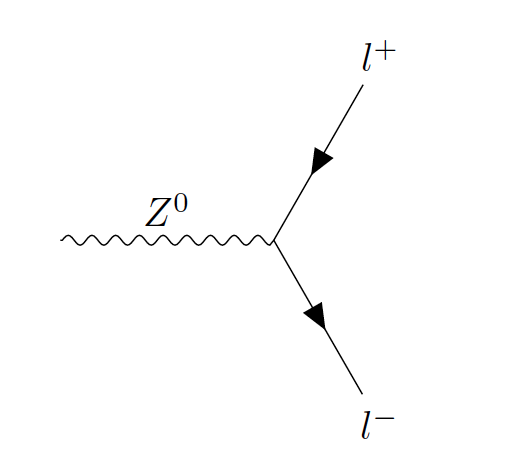
\includegraphics[height=2.5cm]{feynm_Z}
\caption{Feynman diagram for ${Z}^{0}$ decay}
\label{fig:feynmzll}
\end{figure}

For the single Z analysis the following search criteria were employed:
\begin{itemize}
\item Two leptons with ${p}_{T} > 25$ GeV
\item Leptons must have opposite charge
\item Leptons were required to have same flavour
\end{itemize}
\pagebreak
\begin{flushleft}
\textbf{$Z \quad \rightarrow \quad { e }^{ - } \quad + \quad { e }^{ + }$}
\end{flushleft}

The Zee process is one of the main background processes when trying to extract events with two electrons in their final state since it has a relatively high cross section. In order to filter specifically for Zee processes the two leptons were required to be of lepton type 11, which stands for electrons. The results of running this search on the Zee MC simulation are shown below. Fig. \ref{fig:invmzee} plots the frequency distribution against the invariant mass of the two electrons and a distinct peak at $\sim$90 GeV can be seen, which is a good estimate for the Z mass.\\

\begin{figure}
\centering
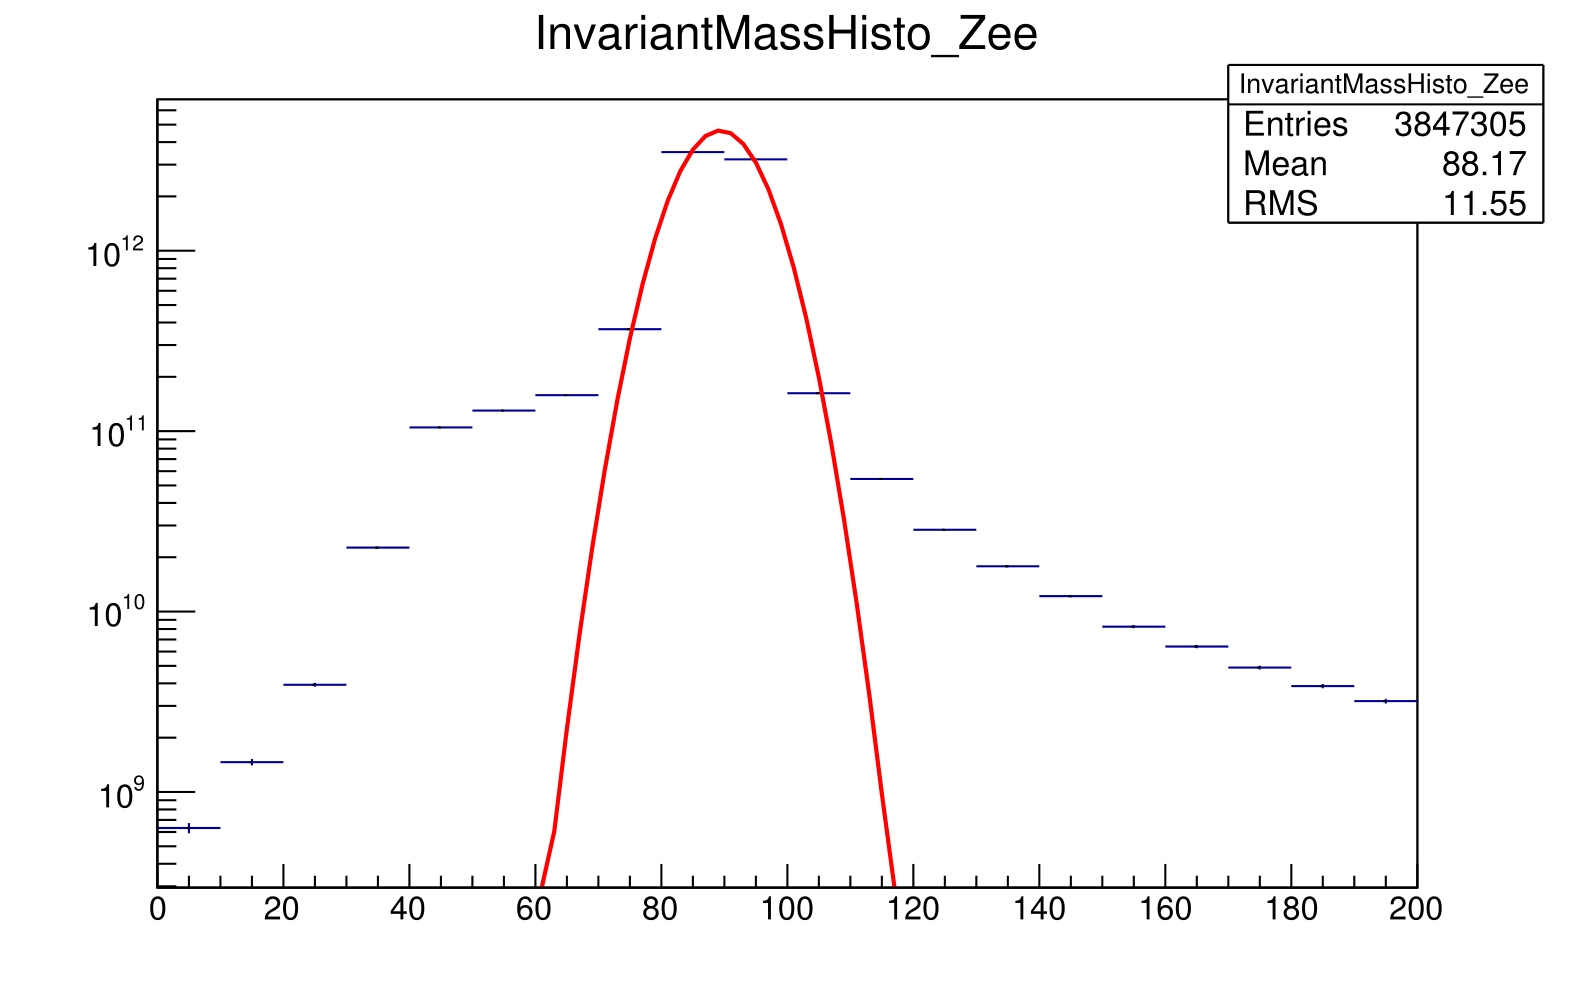
\includegraphics[height=4cm]{InvM_Zee_fit}
\caption{Invariant mass histogram for Zee decay}
\label{fig:invmzee}
\end{figure}

The analysis of background processes also requires the familiarization with plots of different variables such as $\cancel{\it{E}}_{T}$. This plot, visualized in Fig. \ref{fig:mtezee}, exhibits an exponential decrease in $\cancel{\it{E}}_{T}$ until 200 GeV and flattens out into what is called the tail of the distribution.\\

\begin{figure}
\centering
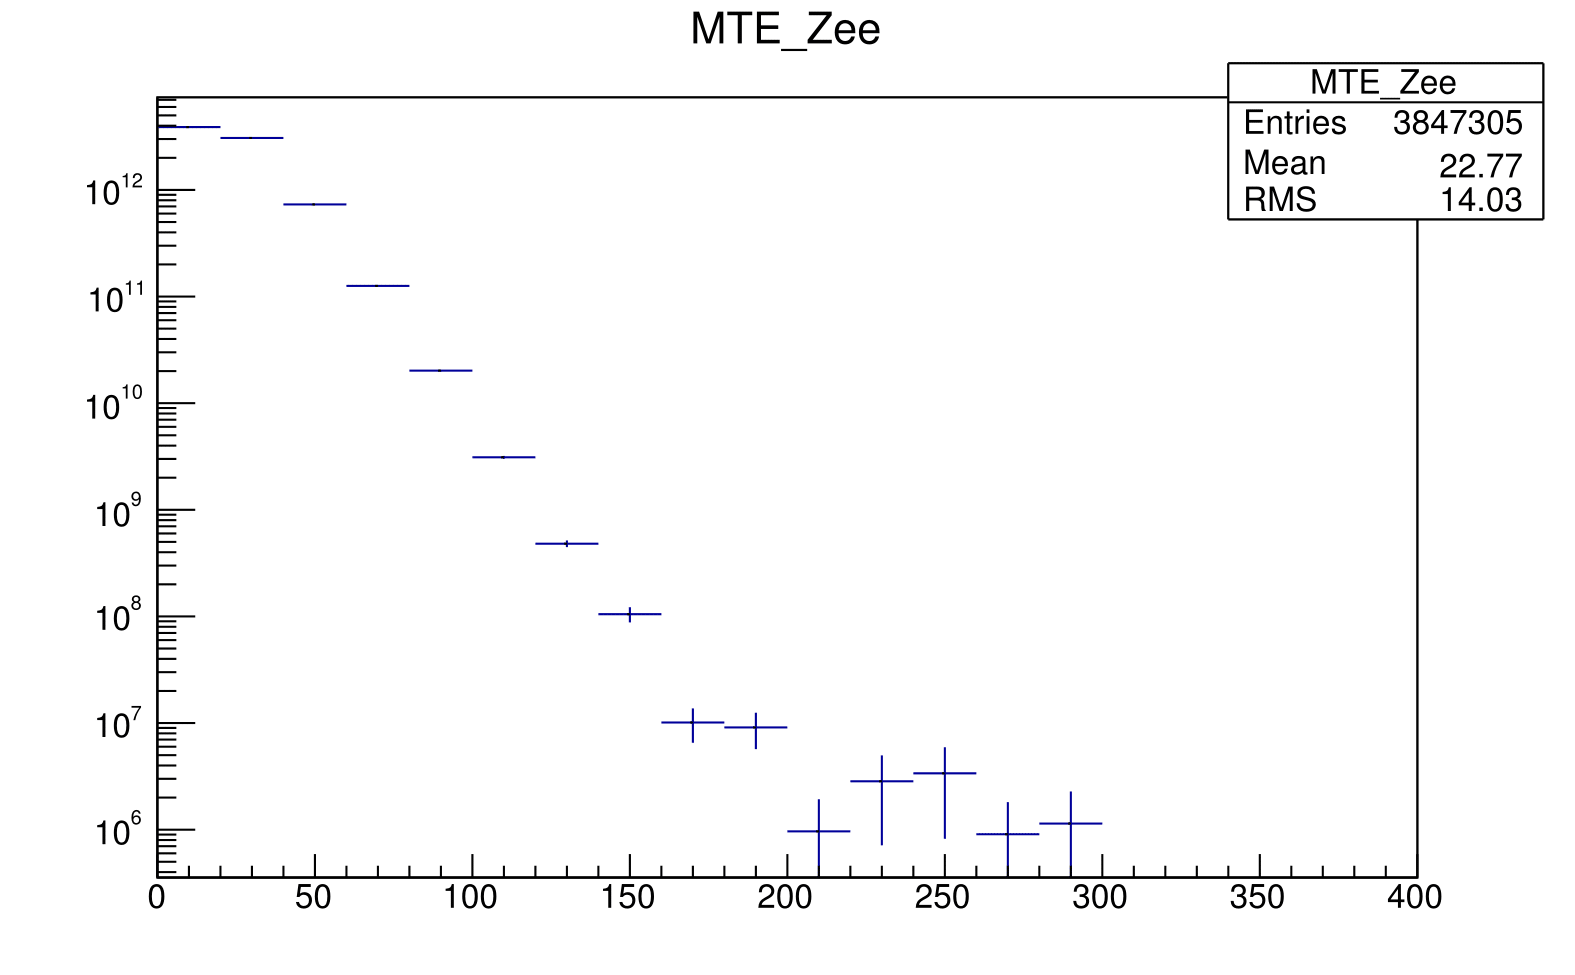
\includegraphics[height=4cm]{MTE_Zee+new}
\caption{$\cancel{\it{E}}_{T}$ for Zee process}
\label{fig:mtezee}
\end{figure}

Furthermore, the number of jets was plotted against frequency and is demonstrated in Fig. \ref{fig:nojzee}. It can be concluded, that small jet multiplicities have a much higher prevalence for Zee processes than large number of jets. All in all, the conducted Zee analysis revealed distinct patterns in the frequency plots of $\cancel{\it{E}}_{T}$, invariant mass and number of jets that can be used to cut on these variables in subsequent searches to suppress the SM background.\\

%% CHECK FOR EXPLANATION FOR NUMBER OF JETS
\begin{figure}
\centering
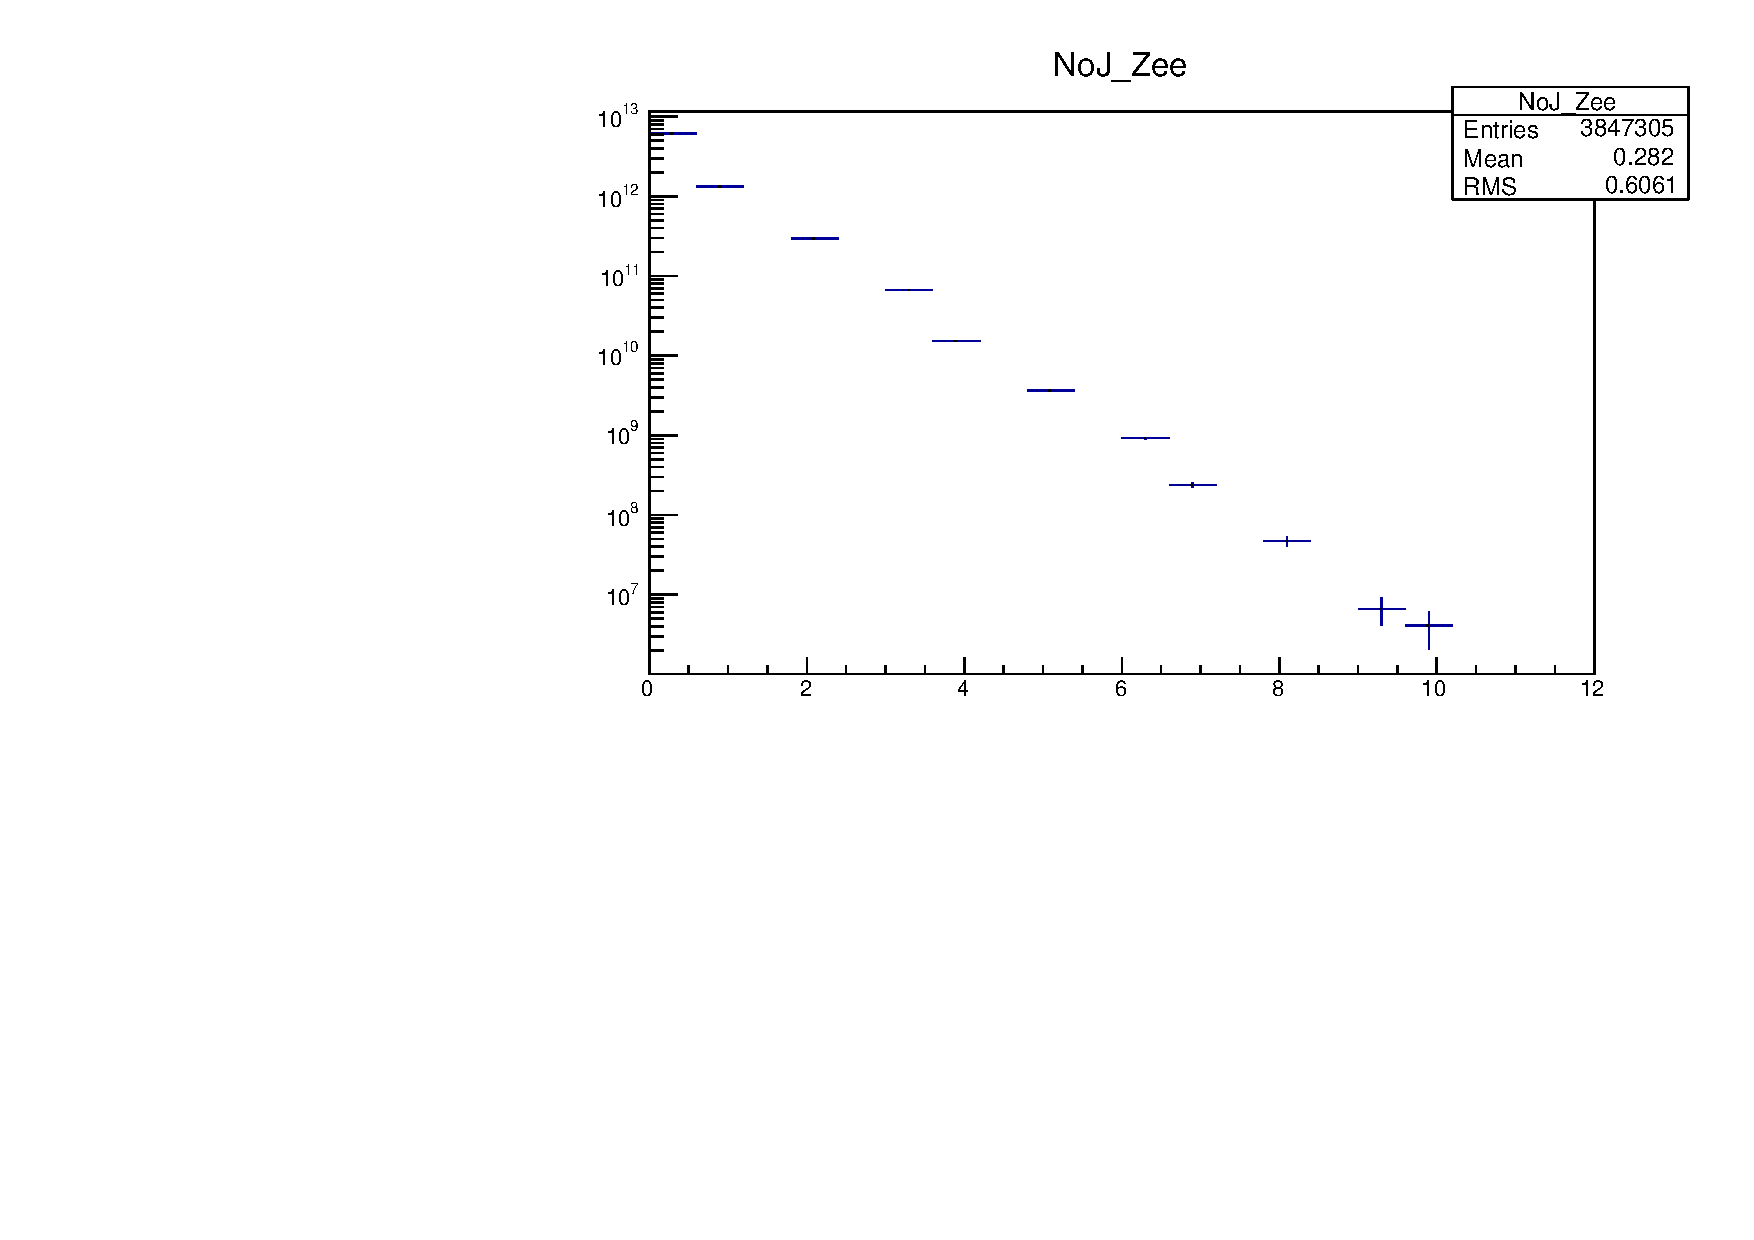
\includegraphics[height=3.7cm]{NoJ_Zee+new}
\caption{Histogram for the number of jets for the Zee process}
\label{fig:nojzee}
\end{figure}
\bigbreak
\begin{flushleft}
$Z\quad \rightarrow \quad { \mu  }^{ - }\quad +\quad { \mu  }^{ + }$
\end{flushleft}
\bigbreak
Since the Z boson can decay into any two leptons of the same flavour, the decay into two muons ($\mu$), each with a mass of 105.7 MeV, also needs to be considered \cite{Agashe:2014kda}. Compared to the previous search, only the lepton type was changed to 13, signifying muons instead of electrons. The search was conducted on the Zmumu MC data set and the invariant mass was again plotted against the frequency distribution and the resulting histogram is shown in Fig. \ref{fig:invmzmumu}. The Gaussian fit clearly shows a peak centered around $\sim$90 GeV which constitutes another good approximation of the Z mass. It should be noted that Fig. \ref{fig:invmzee} and \ref{fig:invmzmumu} look very similar, implying that the two processes have roughly the same cross section.\\

\begin{figure}
\centering
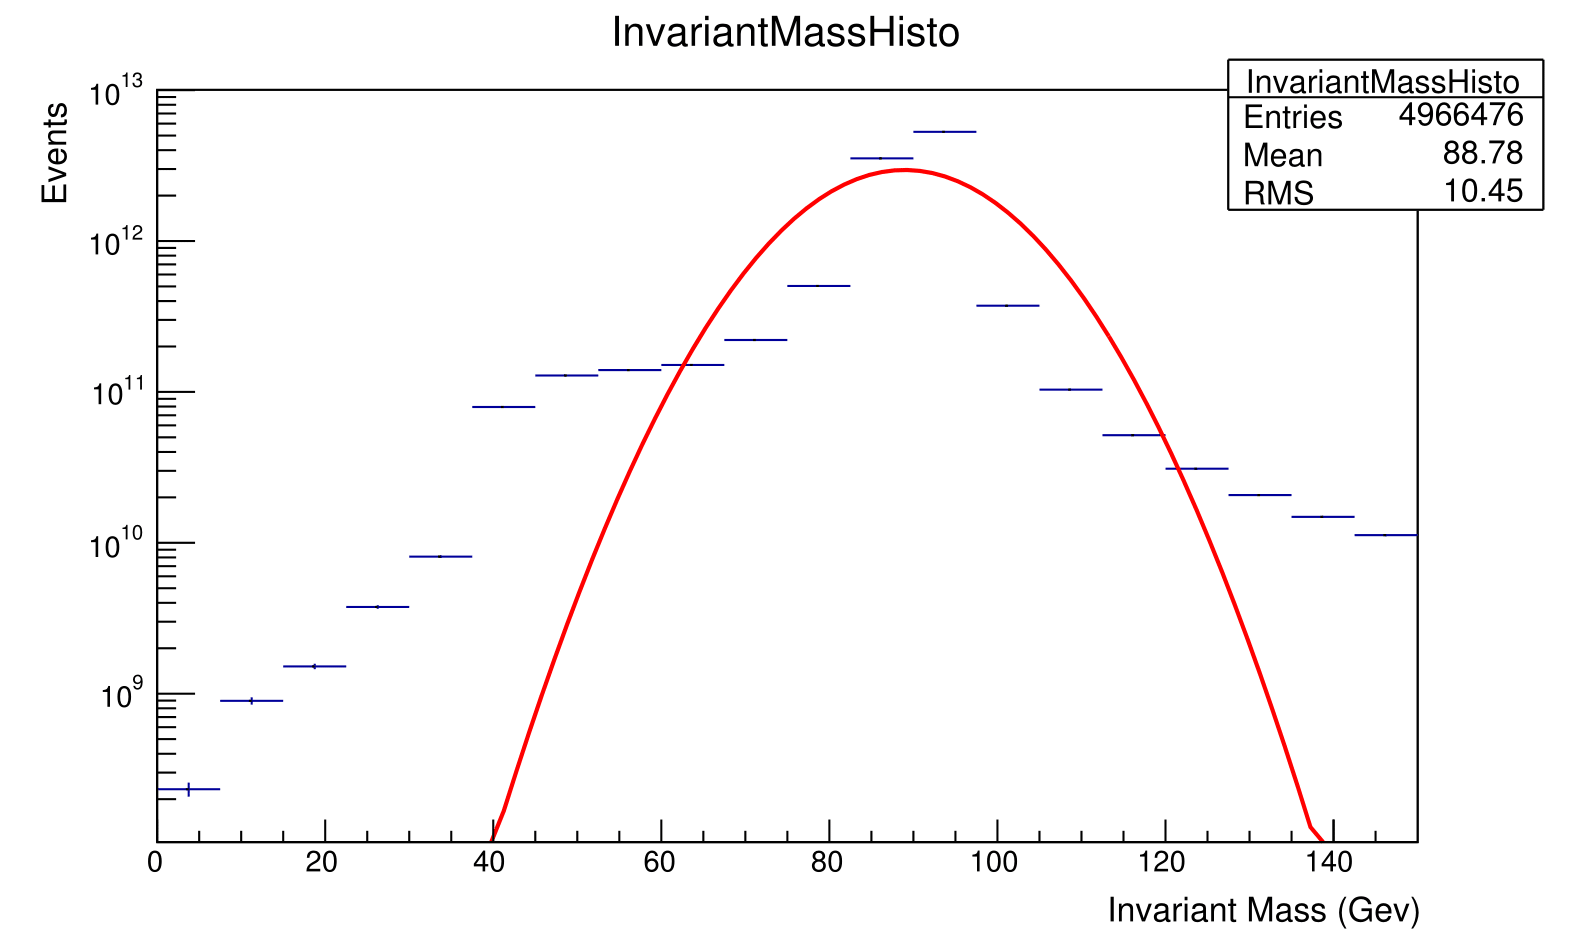
\includegraphics[height=3.7cm]{InvM_Zmumu_fit}
\caption{Invariant mass histogram for Zmumu decay}
\label{fig:invmzmumu}
\end{figure}

Fig. \ref{fig:mtezmumu} shows the $\cancel{\it{E}}_{T}$ histogram for Zmumu. It should be noted that Fig. \ref{fig:mtezee} and \ref{fig:mtezmumu} look very similar because they both display 'fake' $\cancel{\it{E}}_{T}$ which is due to inaccuracies of the detectors and misclassified jet energies. Since neither Zee nor Zmumu contain neutrinos in their final states approximately the same 'fake' $\cancel{\it{E}}_{T}$ distribution is expected and confirmed by Fig. \ref{fig:mtezee} and \ref{fig:mtezmumu}. After a small peak at 30 GeV the $\cancel{\it{E}}_{T}$ frequency exponentially approaches zero and most $\cancel{\it{E}}_{T}$ is found below 100 GeV. A distinct feature of 'fake' $\cancel{\it{E}}_{T}$ is its small tails in the $\cancel{\it{E}}_{T}$ histogram as seen in Fig. \ref{fig:mtezmumu} \cite{pizio2010missing}.\\

\begin{figure}
\centering
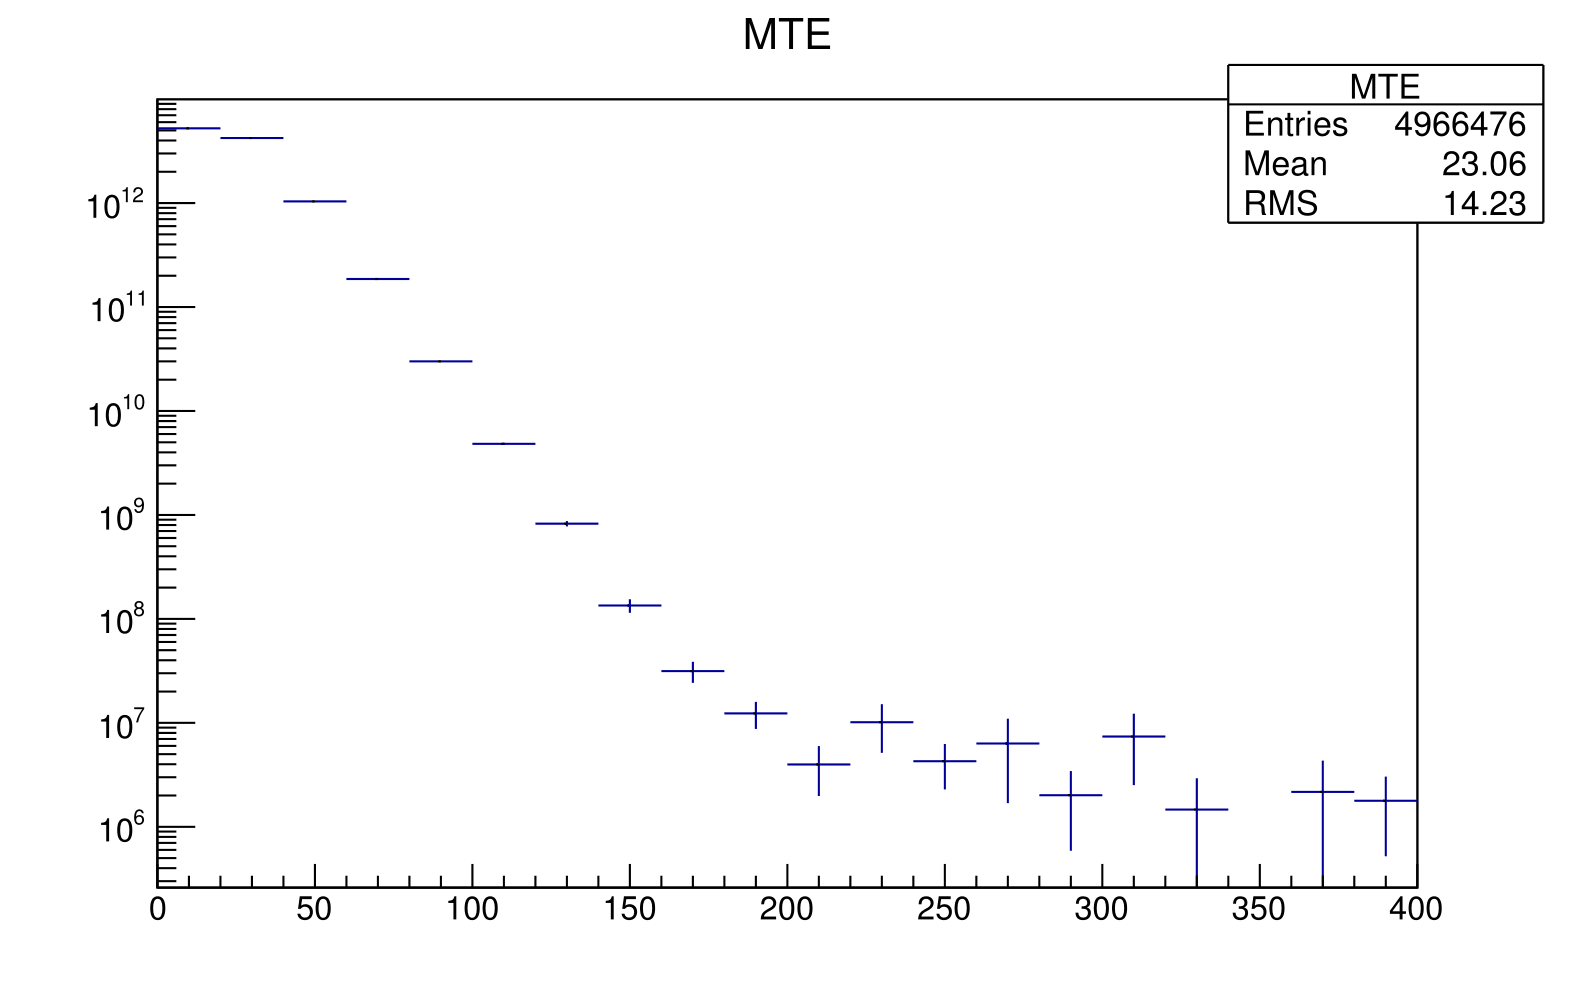
\includegraphics[height=3.7cm]{MTE_Zmumu_new}
\caption{Missing transverse energy histogram for Zmumu process}
\label{fig:mtezmumu}
\end{figure}

When incorrectly measured jet energy is indeed the cause of the $\cancel{\it{E}}_{T}$ distribution obtained in Fig. \ref{fig:mtezmumu}, it expected that the $\cancel{\it{E}}_{T}$ vector will mostly point in the  direction of the most energetic jet. Therefore, when calculating the difference in azimuthal angle between the $\cancel{\it{E}}_{T}$ vector and the most energetic jet, by definition given by the ${0}^{th}$ entry in the jet\_phi vector, a decreasing frequency distribution is expected with increasing radians. This prediction is verified by the histogram shown in Fig. \ref{fig:deltaphizmumu}. \\

\begin{figure}
\centering
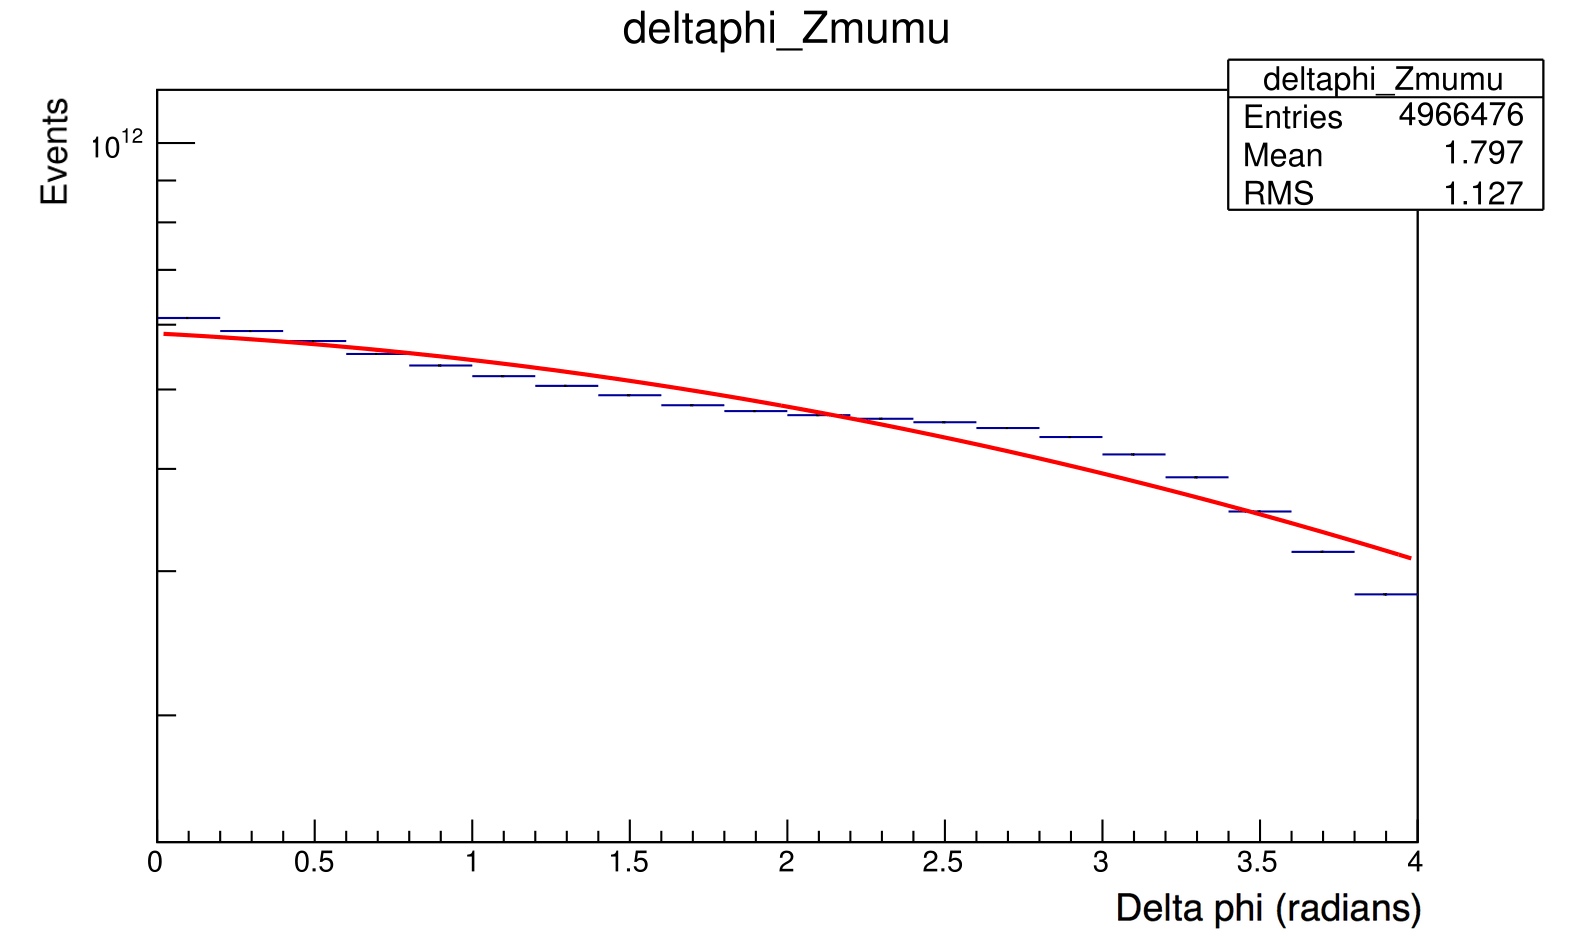
\includegraphics[height=4cm]{deltaphi_jet0_met_Zmumu_fit}
\caption{Distribution of angular difference in azimuthal angle plotted against radians}
\label{fig:deltaphizmumu}
\end{figure}
\bigbreak
\begin{flushleft}
$Z\quad \rightarrow \quad \tau ^{ - }\quad +\quad { \tau  }^{ + }$
\end{flushleft}
\bigbreak
Besides decaying into electrons and muons, the Z boson can also decay into two taus. Since the two tau leptons are very heavy compared to electrons and muons, one might expect the branching fraction of Ztautau to be relatively low. Contrarily, as shown in Fig. \ref{fig:zdecaymodes} the branching fraction of Ztautau is actually even slightly higher than for Zee and Zmumu. However, the Ztautau process still only contributes little background to processes with two leptons in the final state since they decay very quickly either hadronically and leptonically. Furthermore, searching for tau leptons requires much more sophisticated reconstruction methods and it is therefore much more difficult than searching electrons and muons in the final states. Due to all these reasons this decay mode was not searched and analysed further in this paper.\\

\begin{figure}
\centering
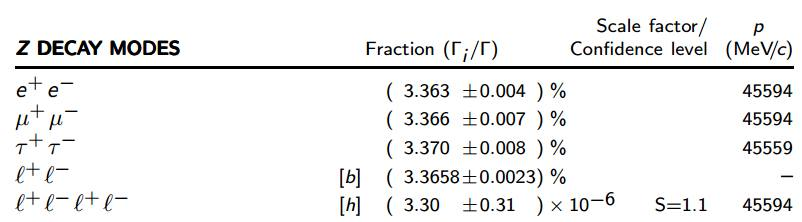
\includegraphics[height=2.5cm]{zdecaymodes}
\caption{Branching fractions for the different Z decay modes}
\label{fig:zdecaymodes}
\end{figure}

%% MARK END

%% ANN START
\subsection{ZZ Decay}

%% DO SEARCH CRITERIA
The decay of two Z bosons is one of the main background processes when searching for the Higgs boson. The decay of ZZ into four leptons (see Fig. \ref{fig:feynmzz}) with ${p}_{T} > 10$ GeV will be looked at.\\

\begin{figure}[H]
\centering
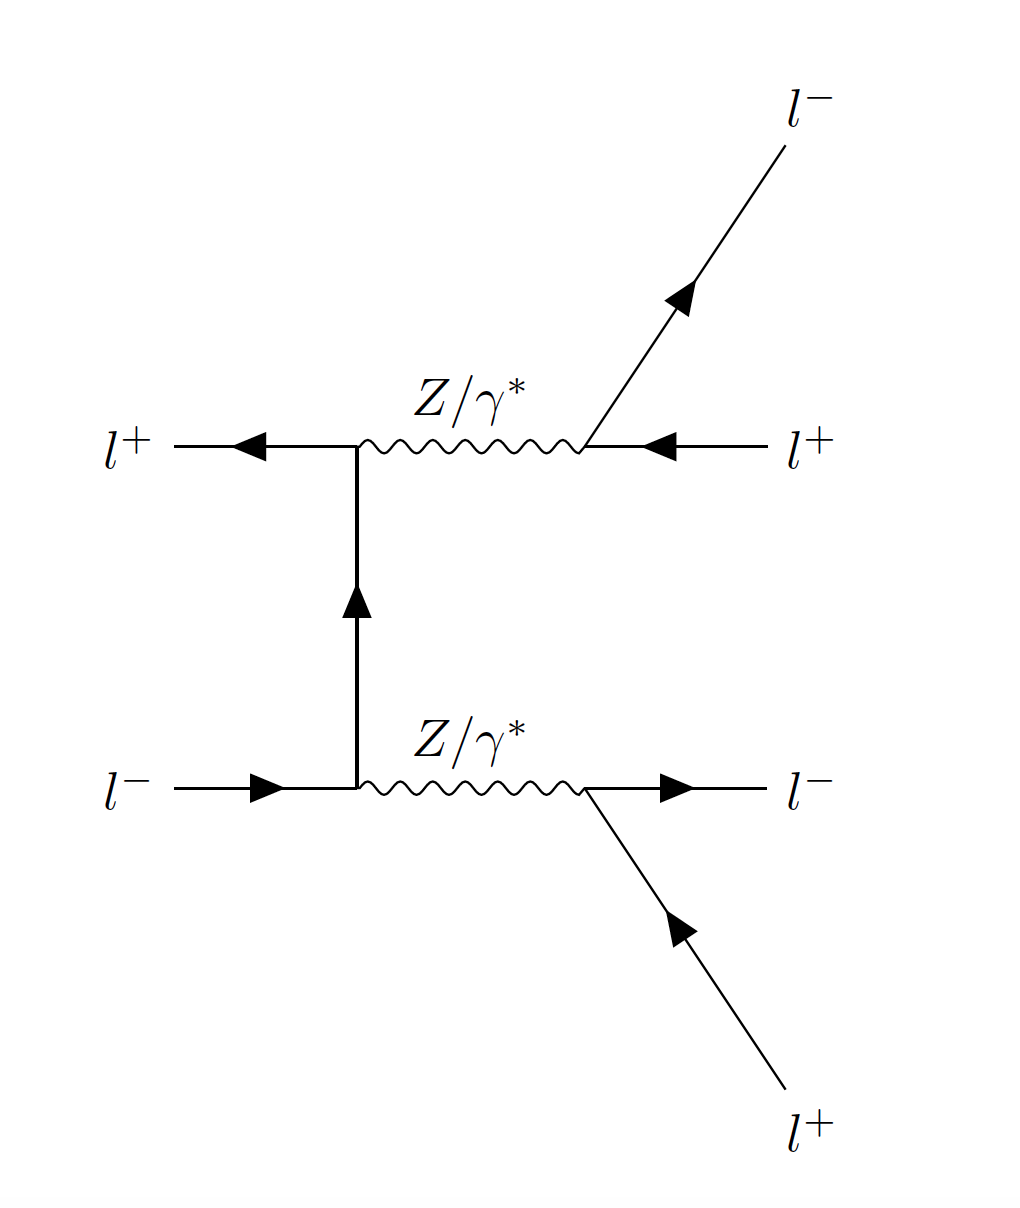
\includegraphics[height=3cm]{feynm_ZZ}
\caption{Feynman diagram for ZZ decay}
\label{fig:feynmzz}
\end{figure}

The two Z candidates were required to decay into lepton pairs of opposite charge and same flavour. Furthermore, the total deviation of the Z candidates from the true mass of the Z boson was set to 20 GeV:\\

\begin{equation}
|mass Z candidate 1 - mass Z| + |mass Z candidate 2 - mass Z| < 20 GeV
\end{equation}

Since the mass of a single Z is equal to $\sim$91.2 GeV, the invariant mass of ZZ is always greater than $\sim$180 GeV \cite{Agashe:2014kda}. This is confirmed in Fig. \ref{fig:invmzz}. As it can be seen from the landau fit, the frequency is greatest at $\sim$220 GeV and drops after this point.\\

\begin{figure}[H]
\centering
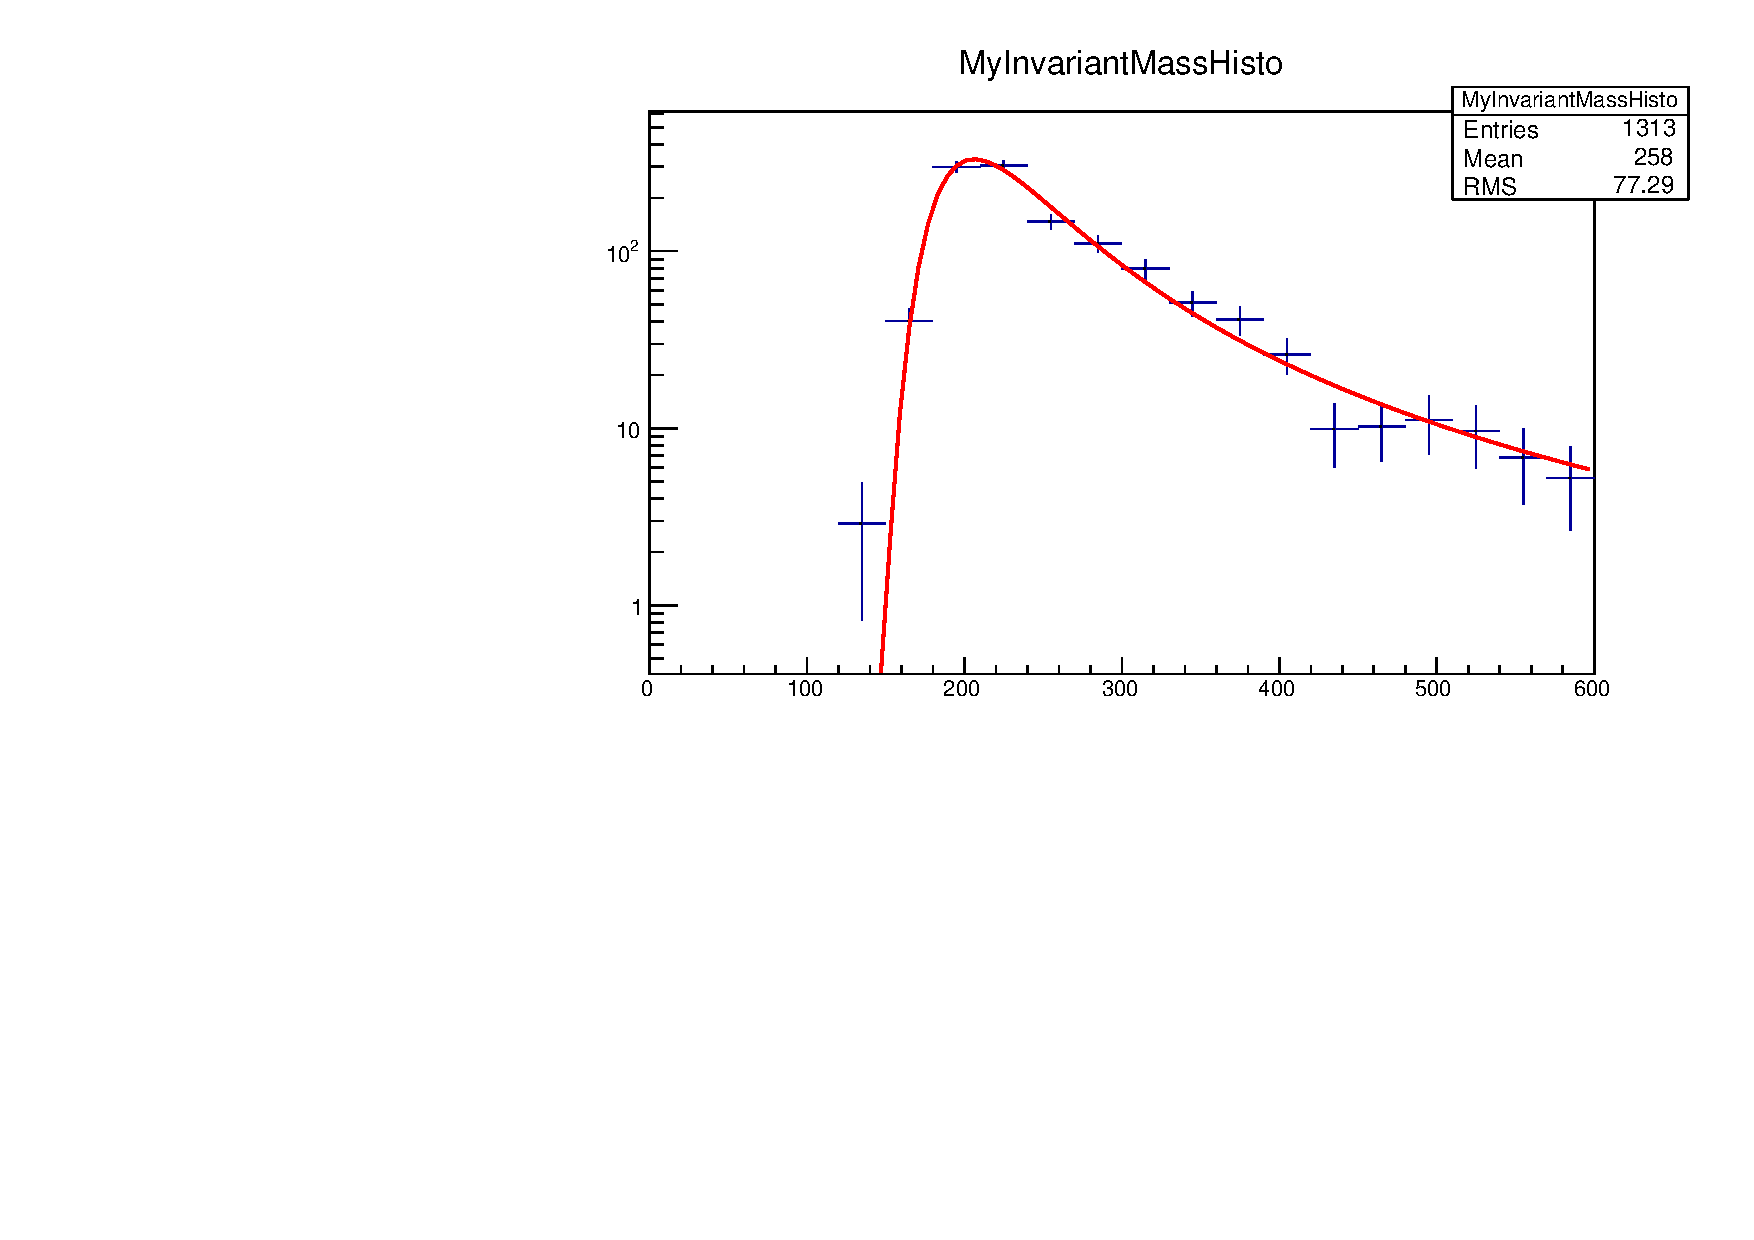
\includegraphics[height=4cm]{MyInvariantMassHistoWtihFit_ZZ}
\caption{Invariant mass histogram for the ZZ decay}
\label{fig:invmzz}
\end{figure}

The number of jets were also plotted, and resulted in a very low number which can be neglected (see Fig. \ref{fig:nojzz}). This result makes sense, because no quarks are produced in the ZZ to 4 leptons process.\\

The $\cancel{\it{E}}_{T}$ histogram is shown in Fig. \ref{fig:mtezz}. Since there are no neutrinos in the final state, no $\cancel{\it{E}}_{T}$ is expected and hence all of the $\cancel{\it{E}}_{T}$ is 'fake'. The histogram exhibits low frequency in the low energy range which is most probably due to incorrectly measured lepton energy.\\

\begin{figure}[H]
\centering
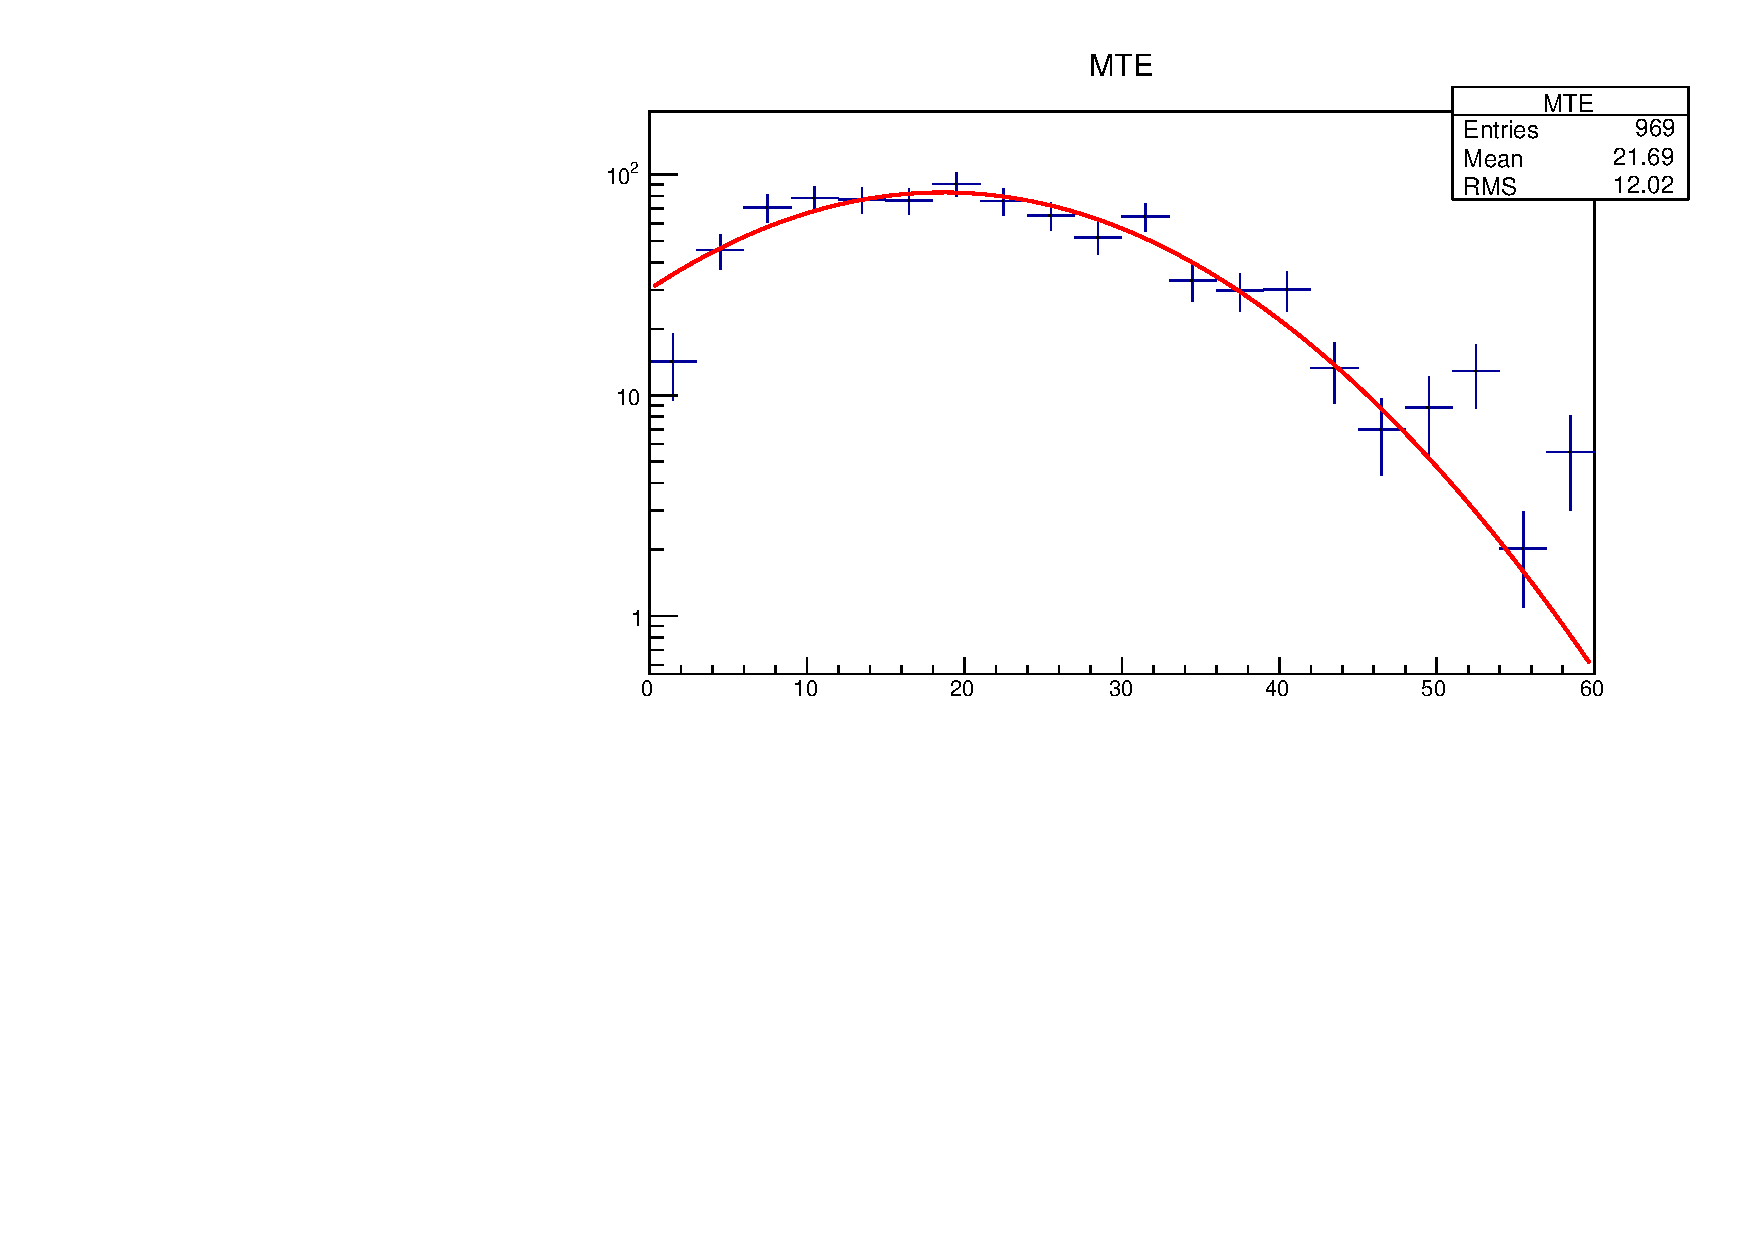
\includegraphics[height=4cm]{MTEWithFit_ZZ}
\caption{$\cancel{\it{E}}_{T}$ for the ZZ process}
\label{fig:mtezz}
\end{figure}

\begin{figure}
\centering
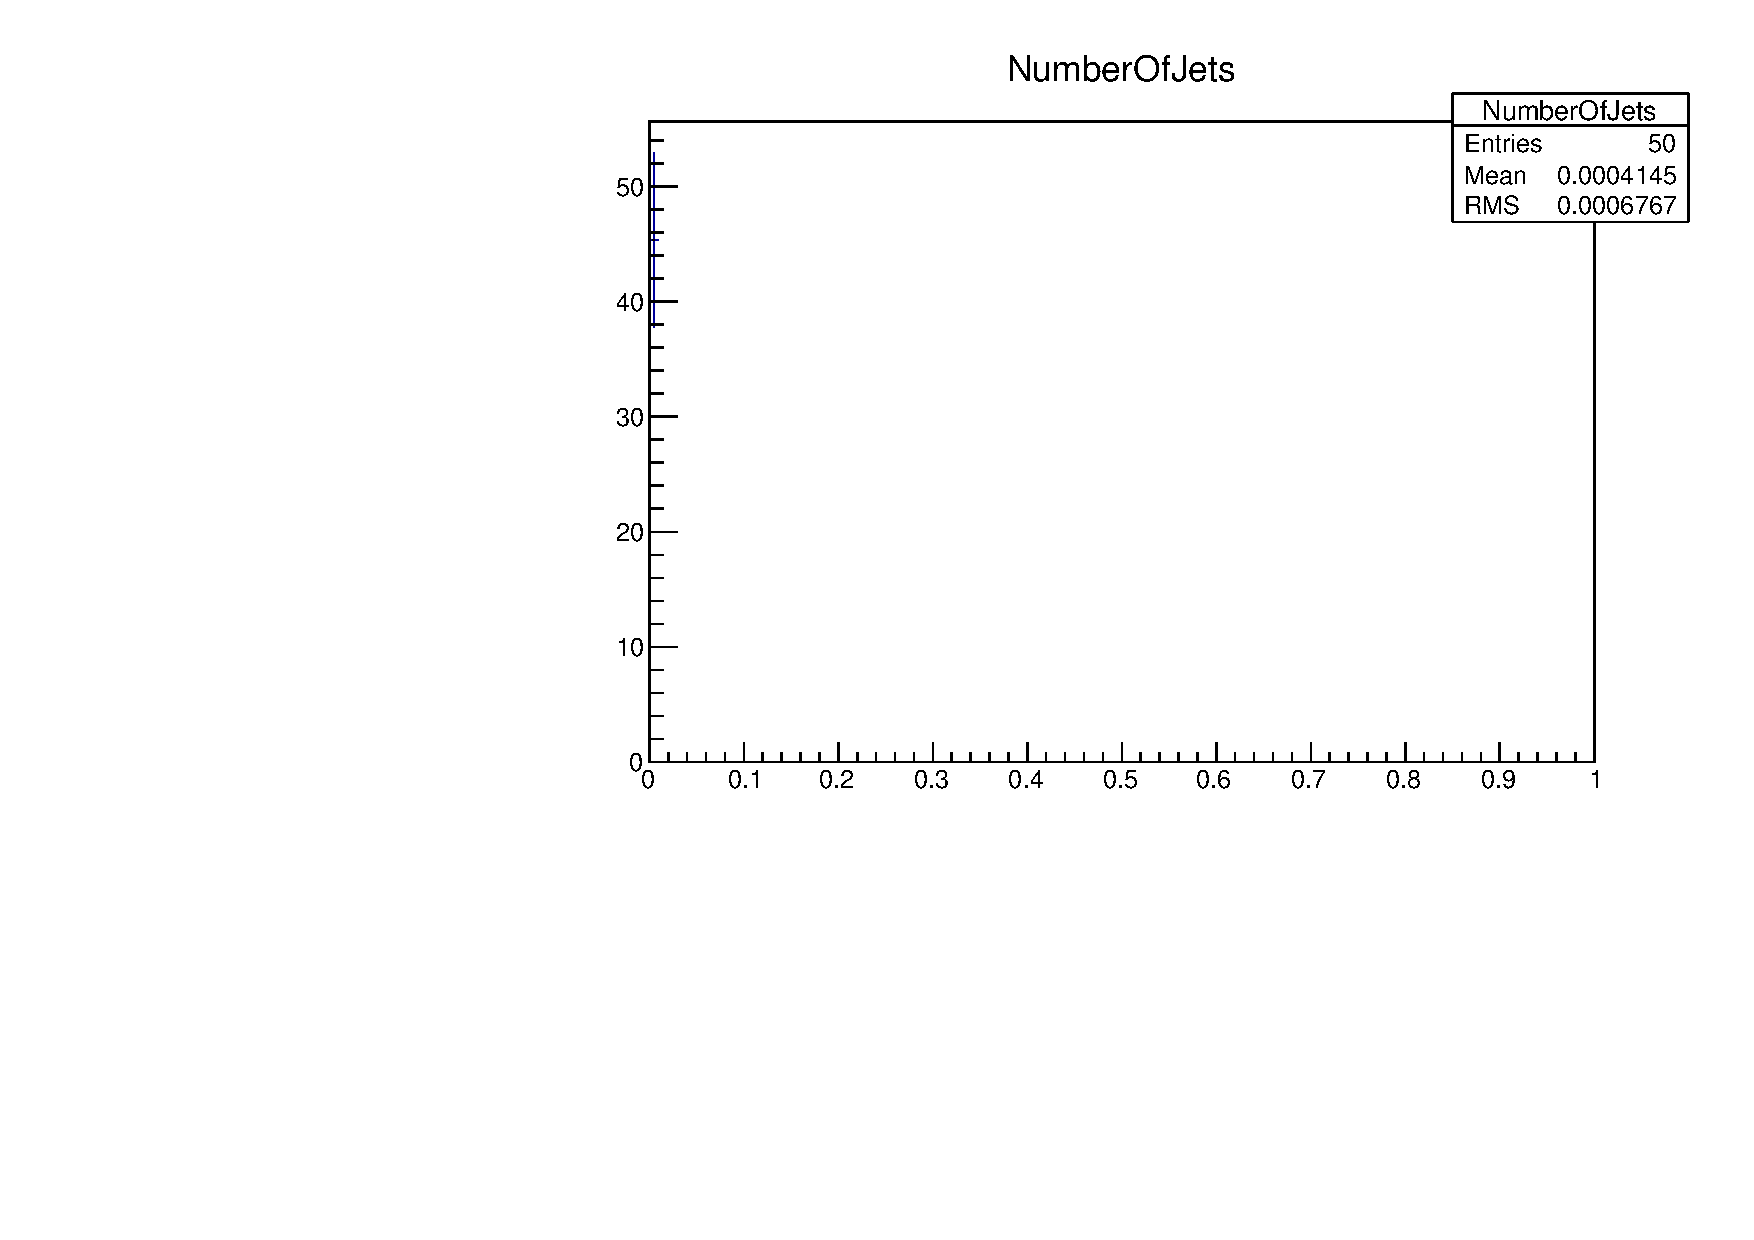
\includegraphics[height=4cm]{NumberOfJets_ZZ}
\caption{Histogram for the number of jets for the ZZ decay}
\label{fig:nojzz}
\end{figure}
%%ANN END

%%MARK START
\subsection{W Decay}

The ${W}^{+}$ and ${W}^{-}$, with integer spin, are the only charged bosons in the SM and together with the neutral Z boson they mediate the weak interaction. W bosons have a mass of $m_{W}\cong 80.4 GeV$ and a cross-section of $\Gamma_{Z}\cong2.1 GeV$. With a branching fraction of $\sim67\%$ the W boson mostly decays hadronically, however, this analysis will only focus on the leptonic decay with $\sim11\%$ branching fraction for each lepton generation \cite{Agashe:2014kda}. Depending on its charge the W boson decays into either a positive lepton and a neutrino or a negative lepton and an anti-neutrino as depicted in the Feynman diagrams below (Fig. \ref{fig:feynmw-} and \ref{fig:feynmw+}). Similar to the Z, the W bosons have a very short half life of $\tau = 1/\Gamma\cong{ 10 }^{ -25 }sec$.\\

\begin{figure}[H]
\centering
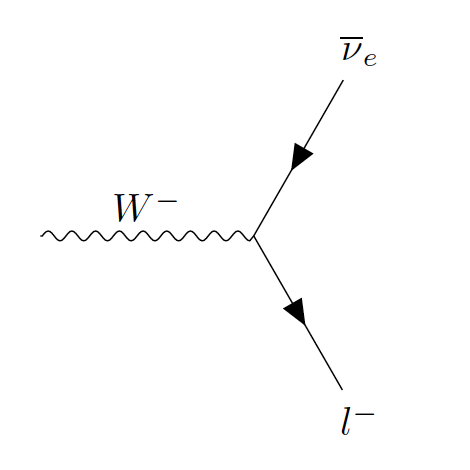
\includegraphics[height=2.5cm]{feynm_W-}
\caption{Feynman diagram for ${W}^{-}$ decay}
\label{fig:feynmw-}
\end{figure}

\begin{figure}[H]
\centering
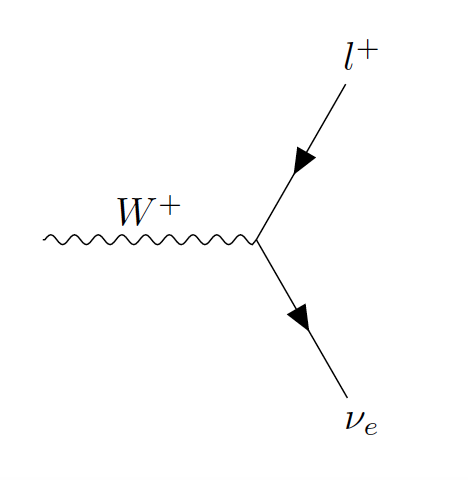
\includegraphics[height=2.5cm]{feynm_W+}
\caption{Feynman diagram for ${W}^{+}$ decay}
\label{fig:feynmw+}
\end{figure}

Contrarily to the Z analysis, no invariant mass histograms can be obtained from the W analysis since only one lepton can be detected and measured in the final state whilst the neutrino escapes the detectors without being measured. Hence, the only way to approximate the momentum of the neutrino is to attribute all the $\cancel{\it{E}}_{T}$ to the neutrino and based on this assumption the ${m}_{T}(W)$ can be calculated.\\

For the single W analysis the following search criteria were employed:
\begin{itemize}
\item Exactly one lepton with ${p}_{T} > 25$ GeV
\item $\cancel{\it{E}}_{T} > 30$ GeV 
\item ${m}_{t}(W) > 30$ GeV
\end{itemize}

The obtained histogram of ${m}_{T}$ is shown in Fig. \ref{fig:mtw} and the Gaussian fit shows a clear peak close to the true W mass given in the literature. Fig. \ref{fig:mtwall} shows the W analysis results that was obtained from all events and visualizes the accuracy of the MC simulation when overlayed with the actual data from the E$\gamma$-channel.\\

\begin{figure}
\centering
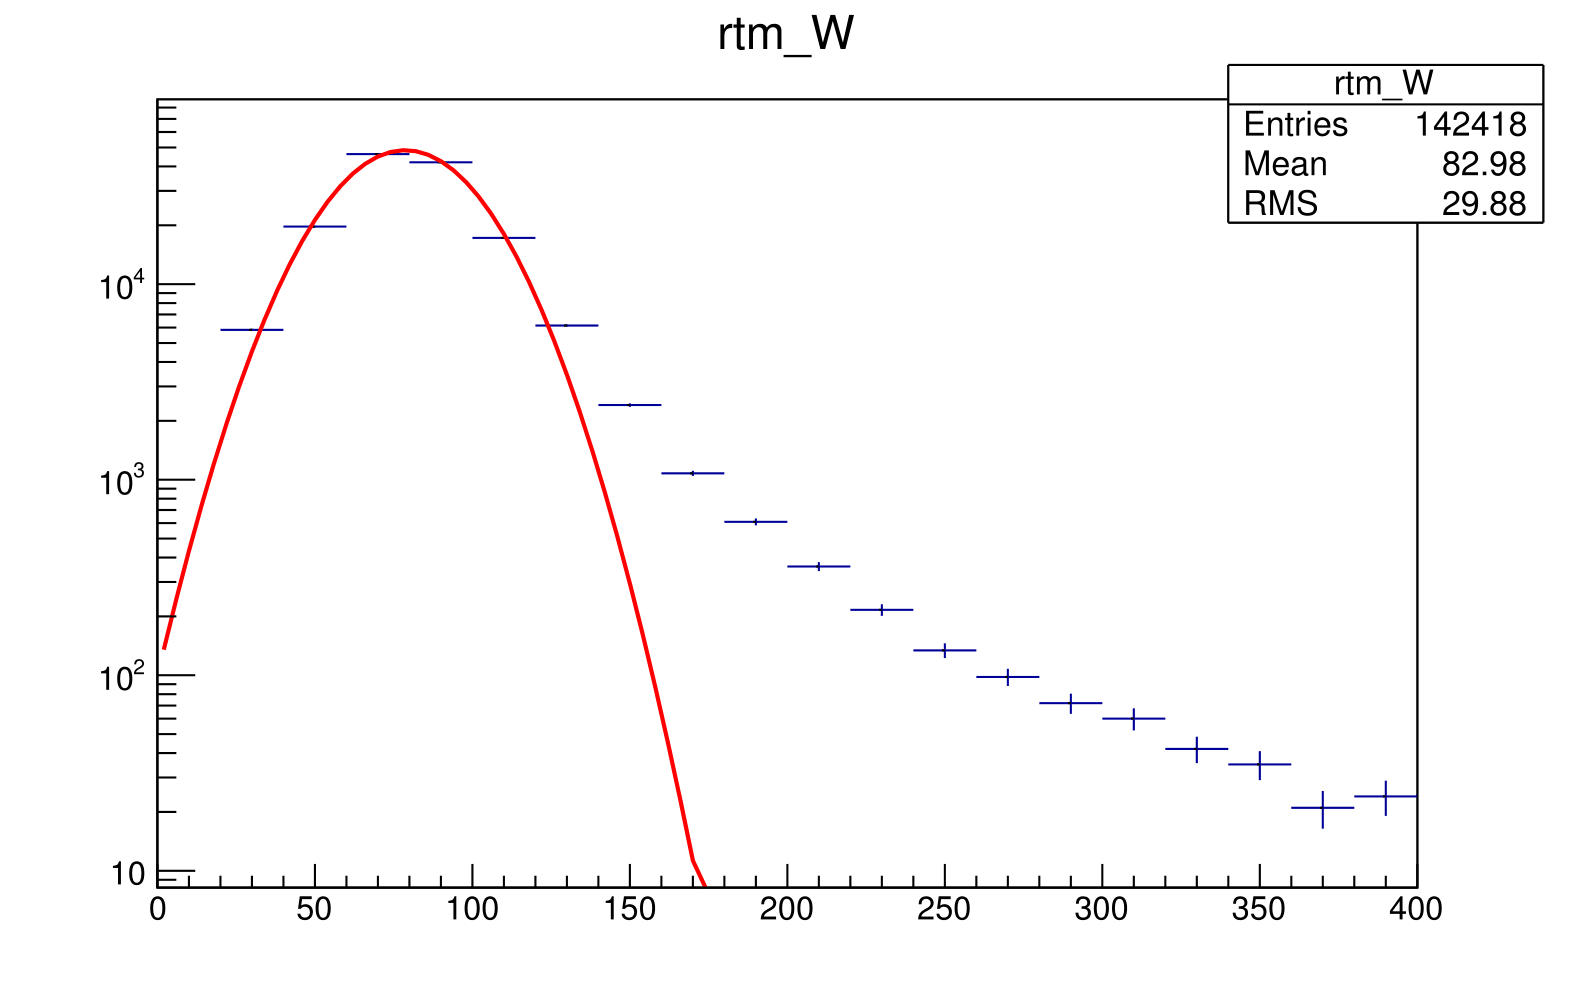
\includegraphics[height=4cm]{W_rtm_fit}
\caption{Histogram of ${m}_{t}$ for the W decay}
\label{fig:mtw}
\end{figure}

\begin{figure}[htbp]
  \begin{center}
    \mbox{
      \subfigure[Distribution of ${m}_{t}$ over all events]{\scalebox{0.28}{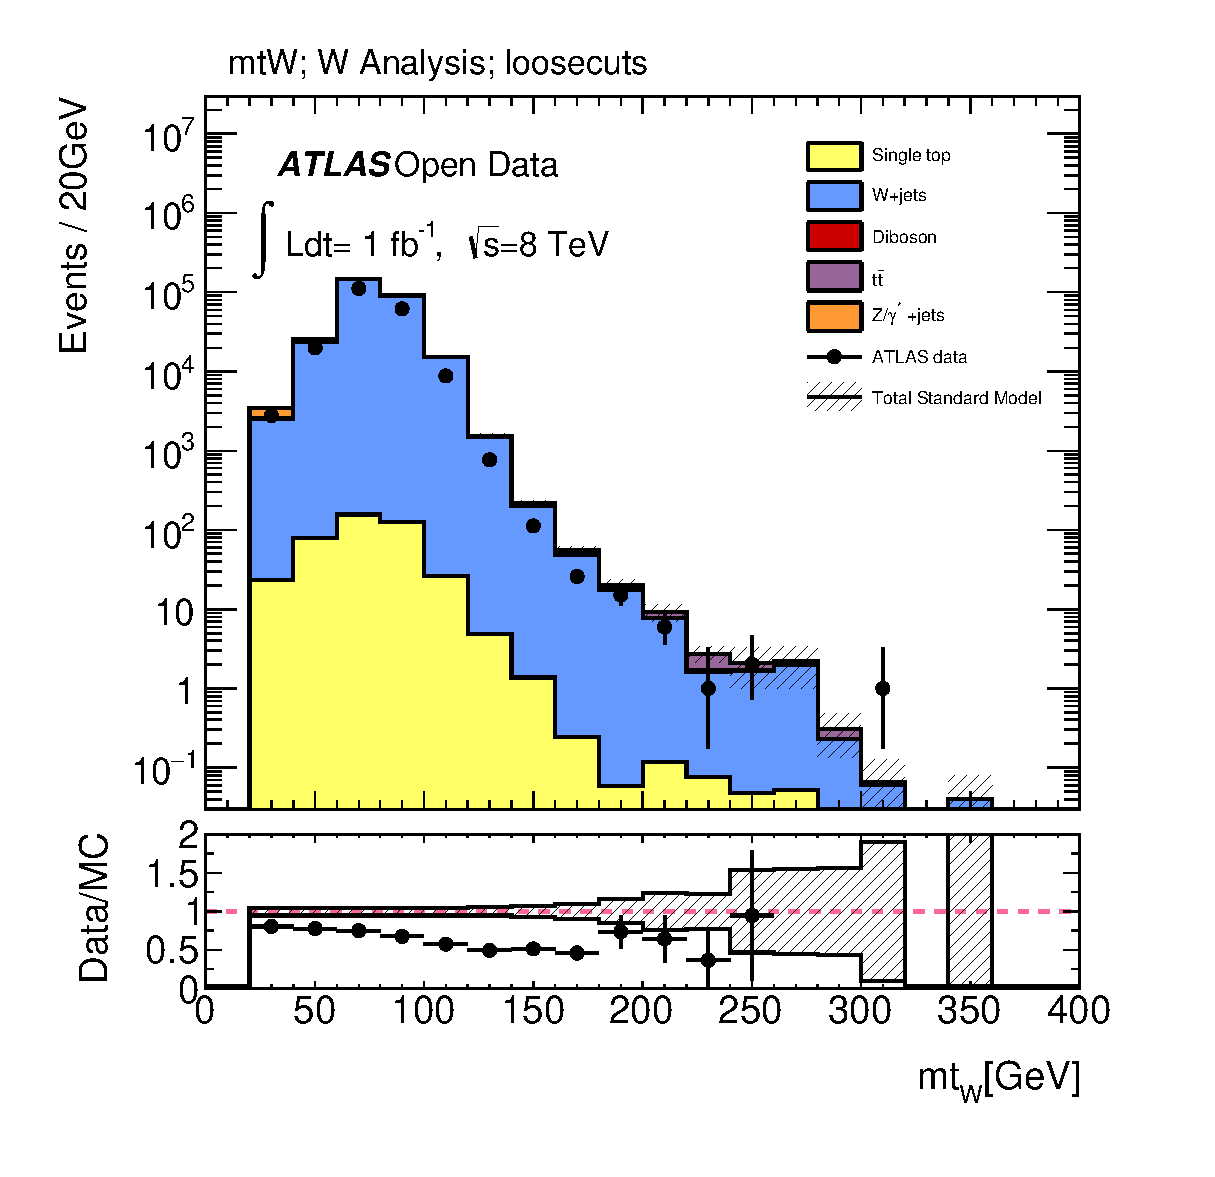
\includegraphics{ee_loosecuts_rtmw}
\label{fig:mtwall}}} \quad
      \subfigure[$\cancel{\it{E}}_{T}$ for the W process]{\scalebox{0.28}{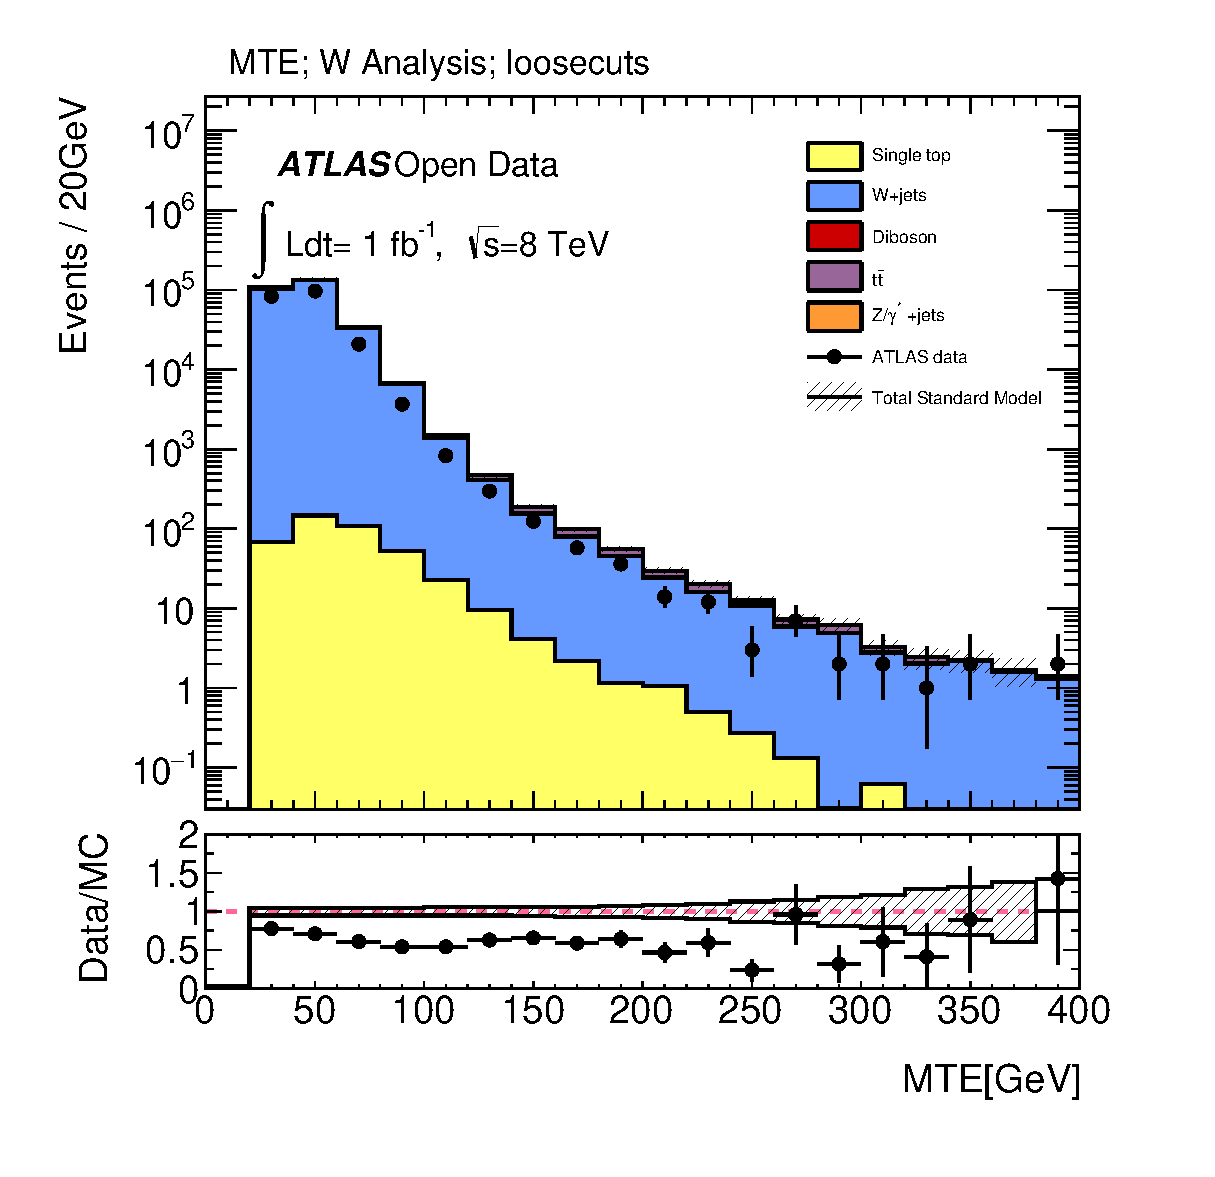
\includegraphics{ee_loosecuts_mtew}\label{fig:mtewall}}}
      }
  \end{center}
\end{figure}

The $\cancel{\it{E}}_{T}$ histogram is shown in Fig. \ref{fig:mtewall} and allows for the same conclusions regarding the accuracy of the MC simulations as Fig. \ref{fig:mtwall}. In contrast to the Z decay, the $\cancel{\it{E}}_{T}$ is considered 'real' since the undetectable neutrino in the final state carries energy.\\


%% MARK END
\pagebreak
%% DHRUVA START
\subsection{WZ Decay}

WZ decay is a diboson mechanism in which a Z and a W boson are produced, which then decay into a lepton pair and a lepton-neutrino pair respectively (see Fig. \ref{fig:WZF}). WZ decays are interesting as they act as a probe for triple gauge couplings. The WZ Analysis searches for events with three leptons and a neutrino (in the form of missing energy). Further selection criteria were as follows: \\

\begin{itemize}
\item There are exactly three leptons with ${p}_{T} > 25$ GeV;
\item WZ candidate is chosen by finding the Z boson candidate closest to the nominal Z
mass
\item $|$mass lepton pair $-$ mass Z $|$$ < 10$ GeV
\item Reconstructed transverse mass W $> 30$ GeV.
\end{itemize}

The first criterion ensures that all detected leptons must have come from a decay involving bosons, as they are relatively heavy and would yield leptons with a momentum above 25 GeV.\\

The second criterion is an algorithm for selecting which leptons come from which bosons. By pairing two leptons at a time, we can simulate a Z boson candidate with an invariant mass that is the same as the invariant mass of the dilepton pair. In the analysis, all three Z candidates (lepton pairs) are compared to find which is closest in mass to the established Z mass. The lepton that is left over is therefore attributed to the decay of the W boson.\\

The third criterion limits the selection to selected Z boson candidates that are less than 10 GeV from the established Z mass.\\

The final criterion allows for off-shell W bosons to be as low as 30 GeV (since the W mass is around 80 GeV), but does not select any W boson candidates that are less than 30 GeV. For more details on how these criteria were implemented, see the WZ section of code in the appendix. \\

The W boson's mass can be reconstructed by calculating ${m}_{T}$ using the third lepton's mass and the neutrino's transverse momentum (missing energy) using Eq. 2.

\begin{figure}
\centering
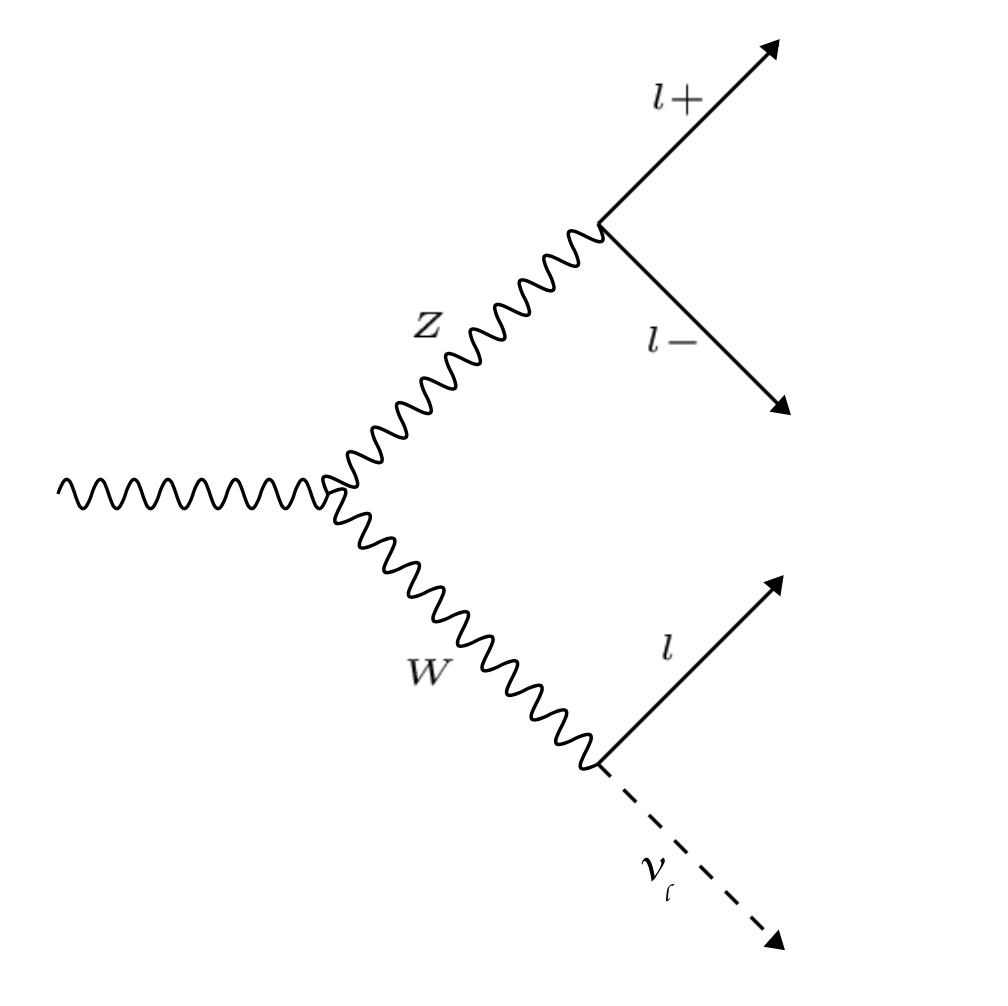
\includegraphics[height=3.5cm]{WZ_feynman.jpg}
\caption{Feynman Diagram for WZ decay}
\label{fig:WZF}
\end{figure}

The results clearly show that the invariant mass graph (Fig. \ref{fig:WZIM}) peaks at 90.1 $\pm$0.185 GeV, which corresponds to the mass of a Z boson which is measured to be 91.1876 GeV \cite{BeringerZ}. The reconstructed mass graph (Fig. \ref{fig:WZMT}) peaks at the 80.0 $\pm$1.40 GeV, which also corresponds to the mass of a W boson which was found to be 80.385 GeV \cite{BeringerW}. Therefore, the analysis selects the correct events we want to look at. \\

\begin{figure}[H]
\centering
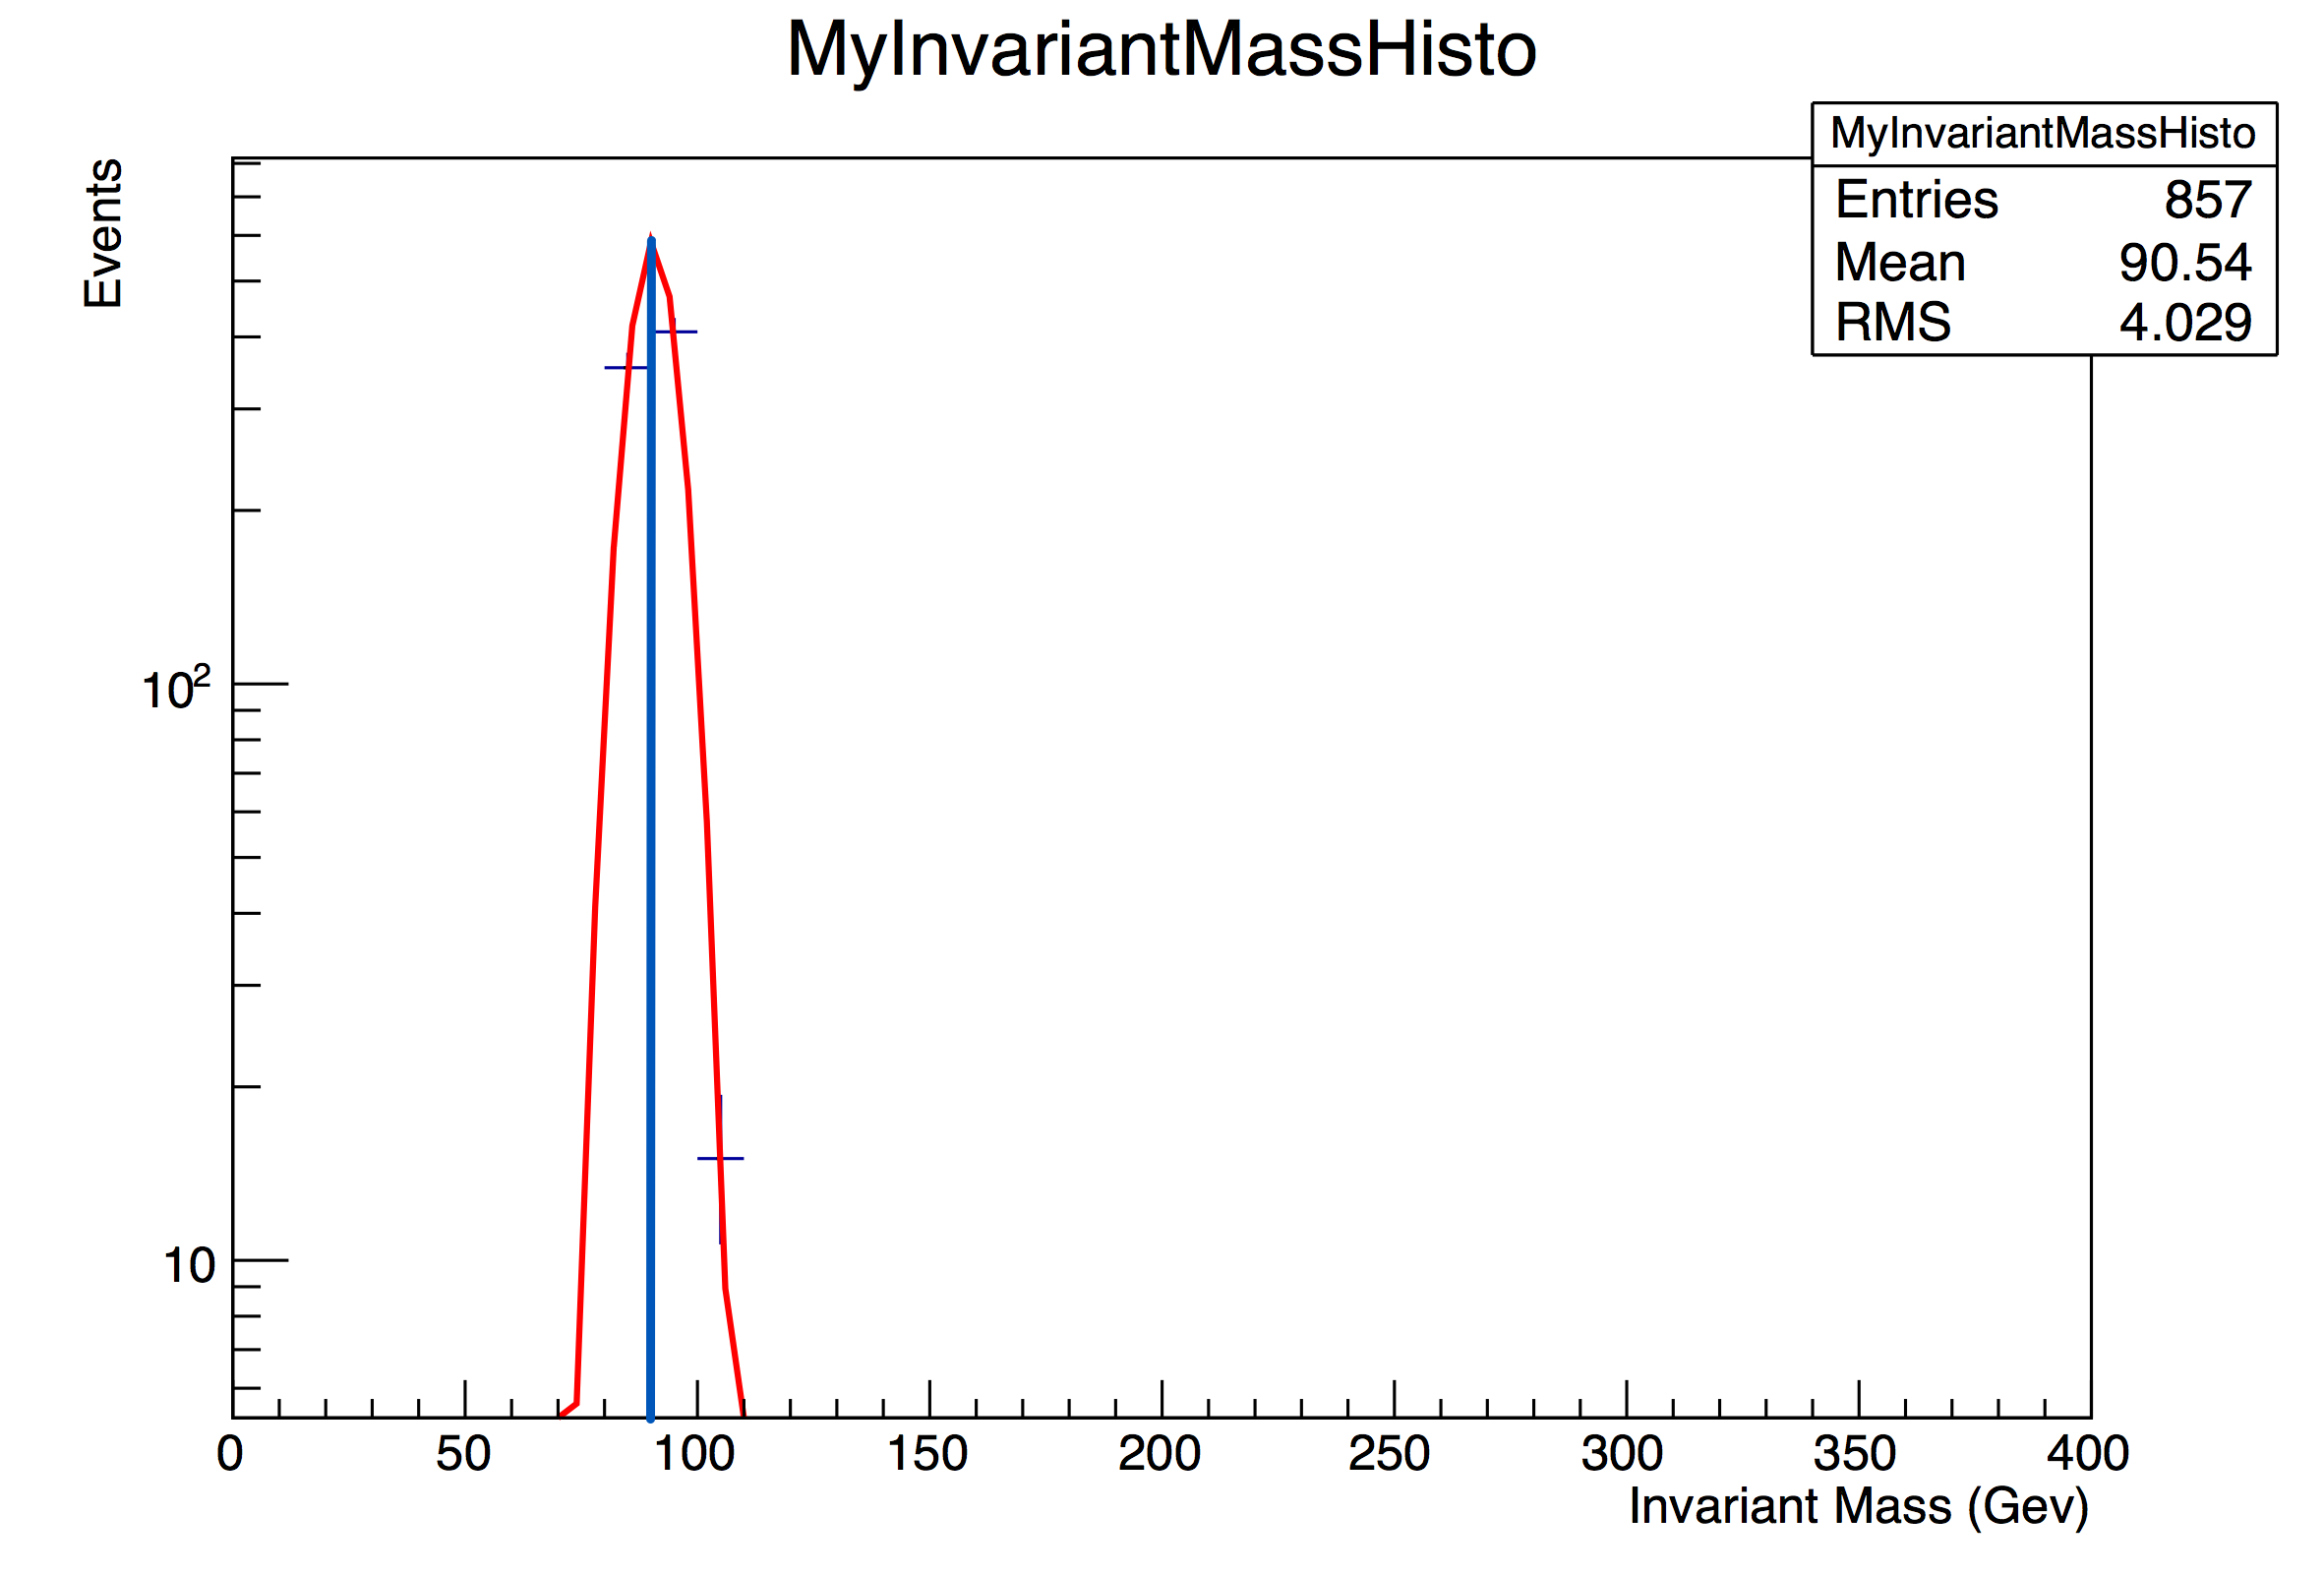
\includegraphics[height=4cm]{WZ_IM.jpg}
\caption{Invariant Mass (Z mass) histogram for WZ decay analysis}
\label{fig:WZIM}
\end{figure}

\begin{figure}[H]
\centering
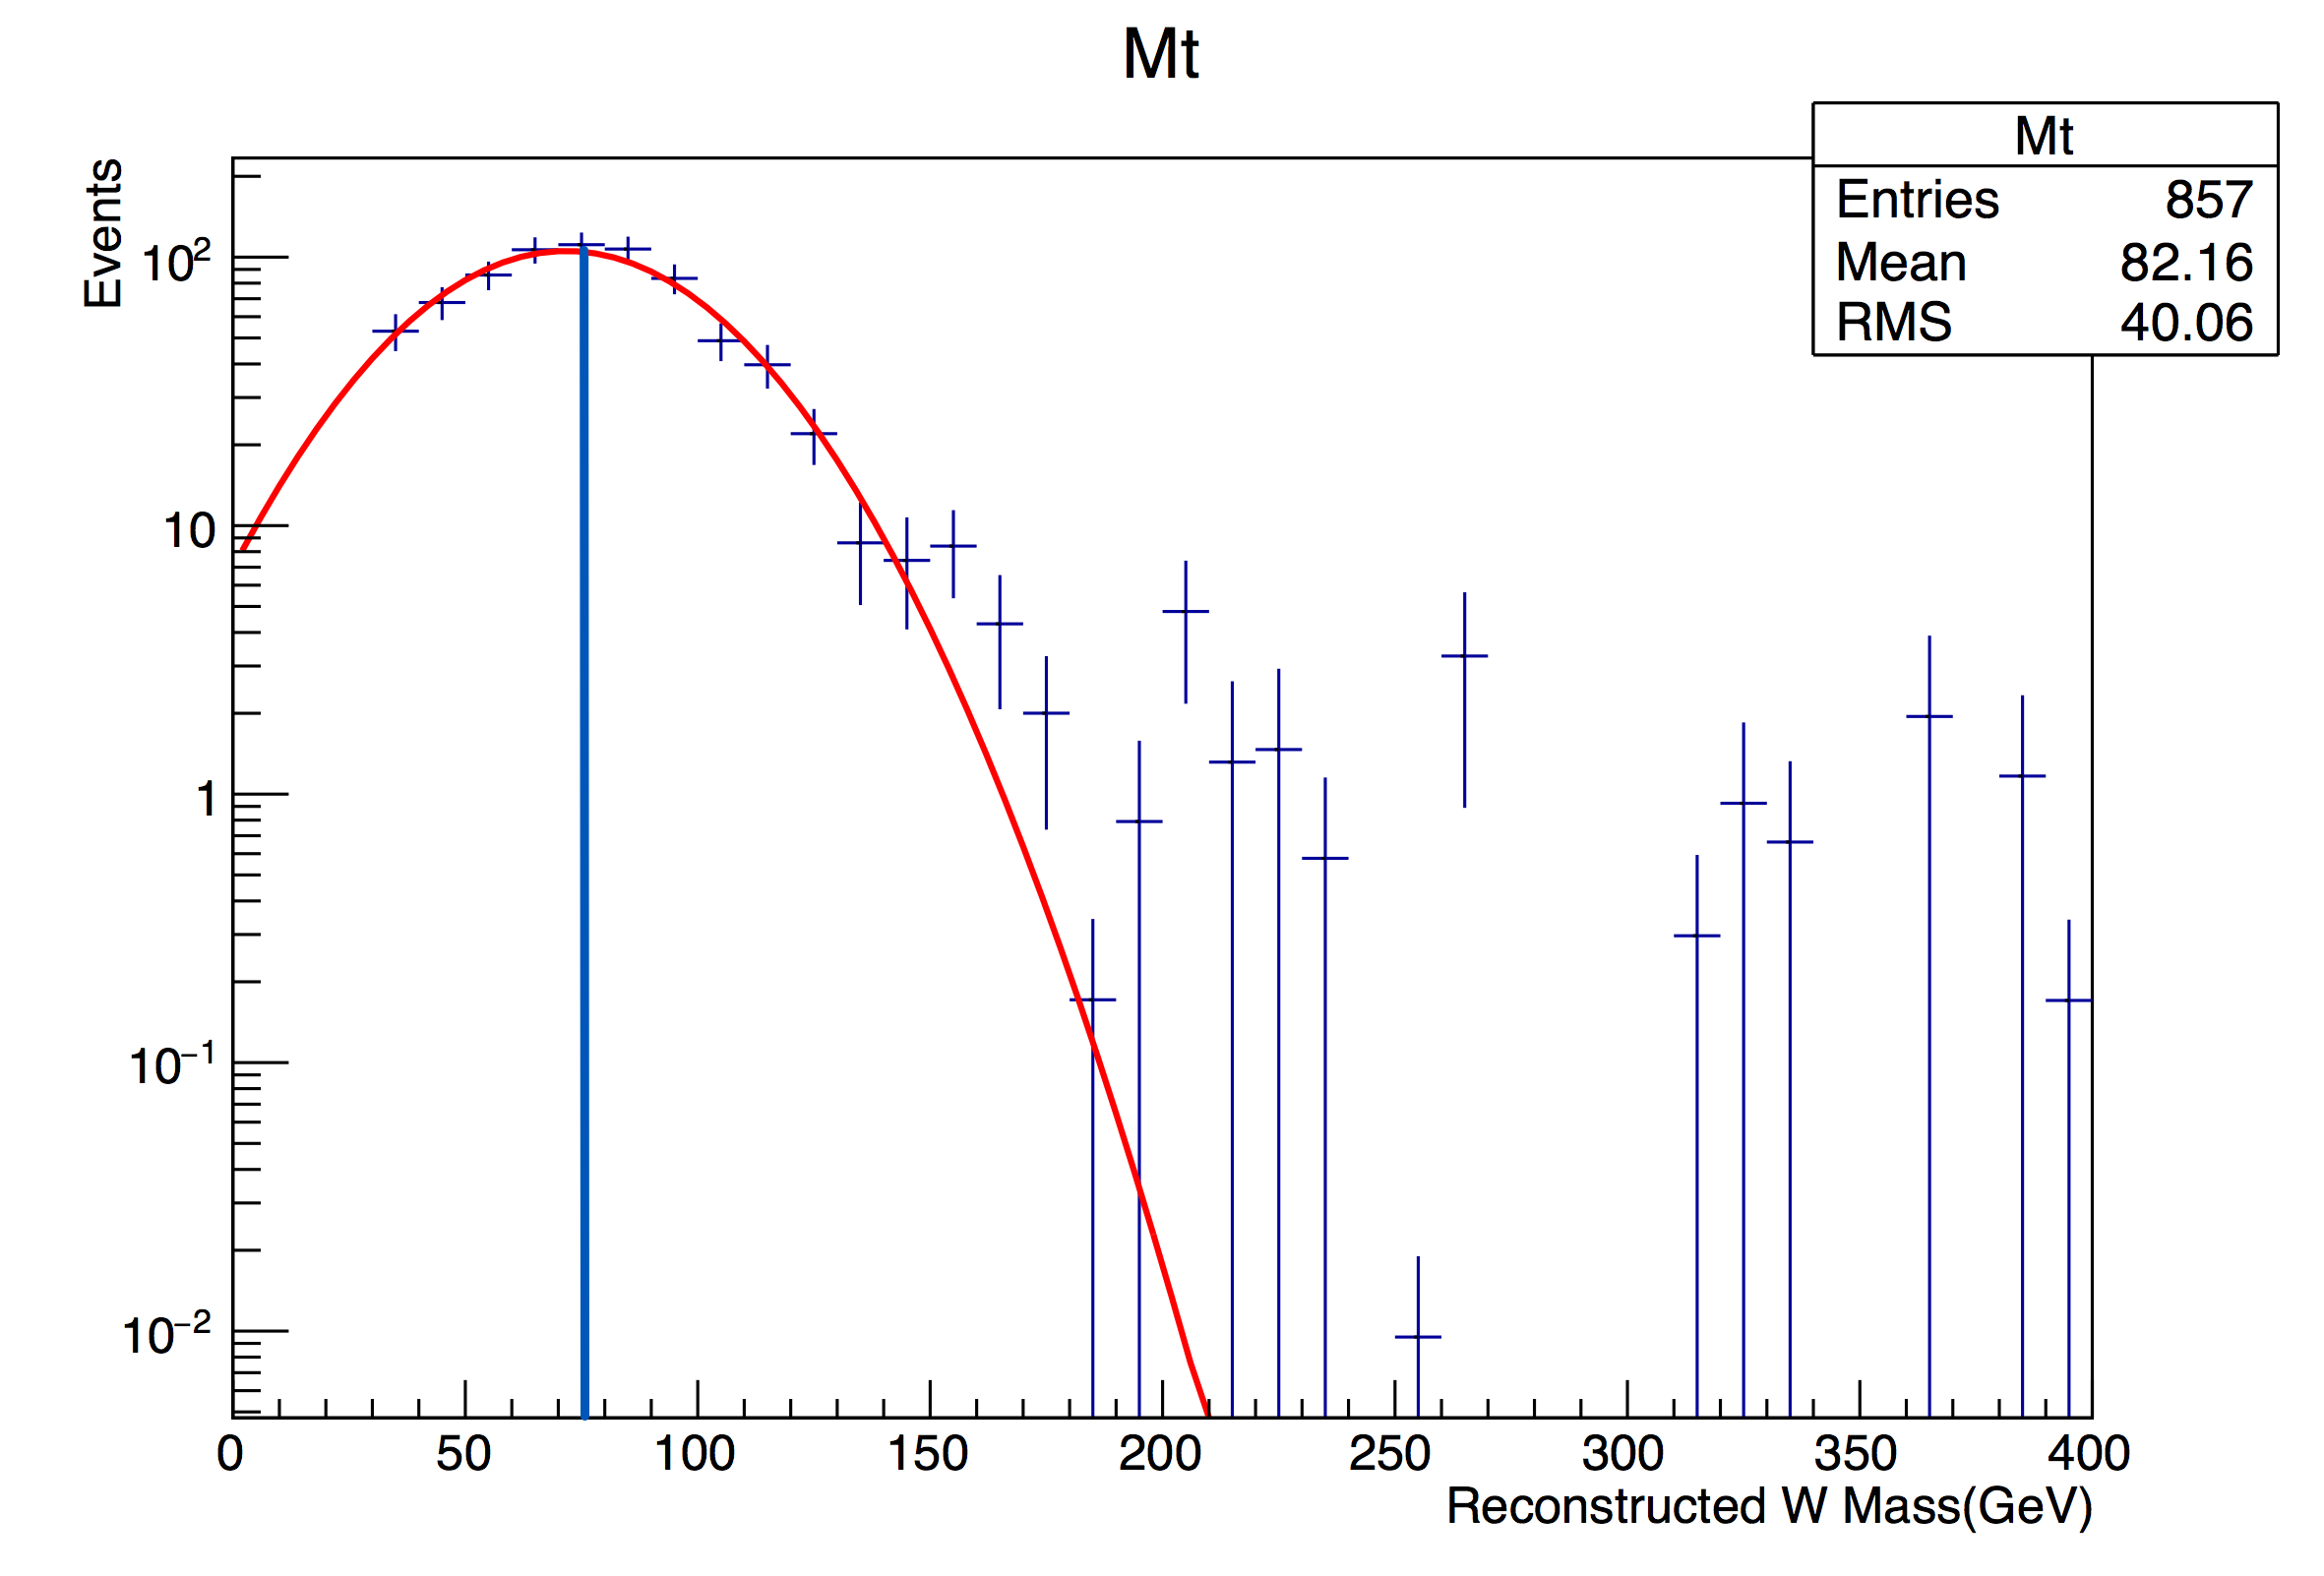
\includegraphics[height=4cm]{WZ_Mt.jpg}
\caption{Reconstructed W mass for WZ decay analysis}
\label{fig:WZMT}
\end{figure}

Out of all run I data that the analysis was run on, only 857 events were WZ decay events. This suggests that the WZ decay is a relatively rare one, and does not contribute significantly to the background processes. \\

%% DHRUVA END

%% SHAM START
\subsection{$t \bar{t}$ Decay}
Top quarks, also known as truth quarks, are the heaviest of all the elementary particles with a mass of ${m}_{t}\cong 173.34GeV$ and a cross section of $\Gamma_Z \cong 64.2 GeV$. \cite{abazov2008simultaneous} As all quarks, the top is a fermion with a spin of $-{1/2}$ and feels all four fundamental forces. In the main channel discussed, the $t\bar{t}$ pair each decay into a b-tagged jet and a W boson. The top's heaviness means that it is highly unstable and has a very short half-life, which is predicted by the SM to be just $\tau = 1/\Gamma\cong{ 10 }^{ -25 }sec$. Strong interactions take about 20 times as long and therefore the top cannot form hadrons. This is a unique property of the top as all other quarks hadronize, or couple to other quarks to form hadrons. By far, the top decays most commonly to a bottom quark or b-tagged with a branching fraction of $\sim99.8\%$ \cite{Agashe:2014kda}. Top-antitop pairs are created by highly energetic gluon decay processes.\\

For the top-antitop pair analysis the following search criteria were employed:
\begin{itemize}
\item Exactly one lepton with $p_\tau > 25$ GeV
\item At least four jets
\item At least two b-tagged jets
\item $\cancel{\it{E}}_{T} > 30$ GeV
\item ${m}_{T}(W) > 30$ GeV
\end{itemize}

\begin{figure}
\centering
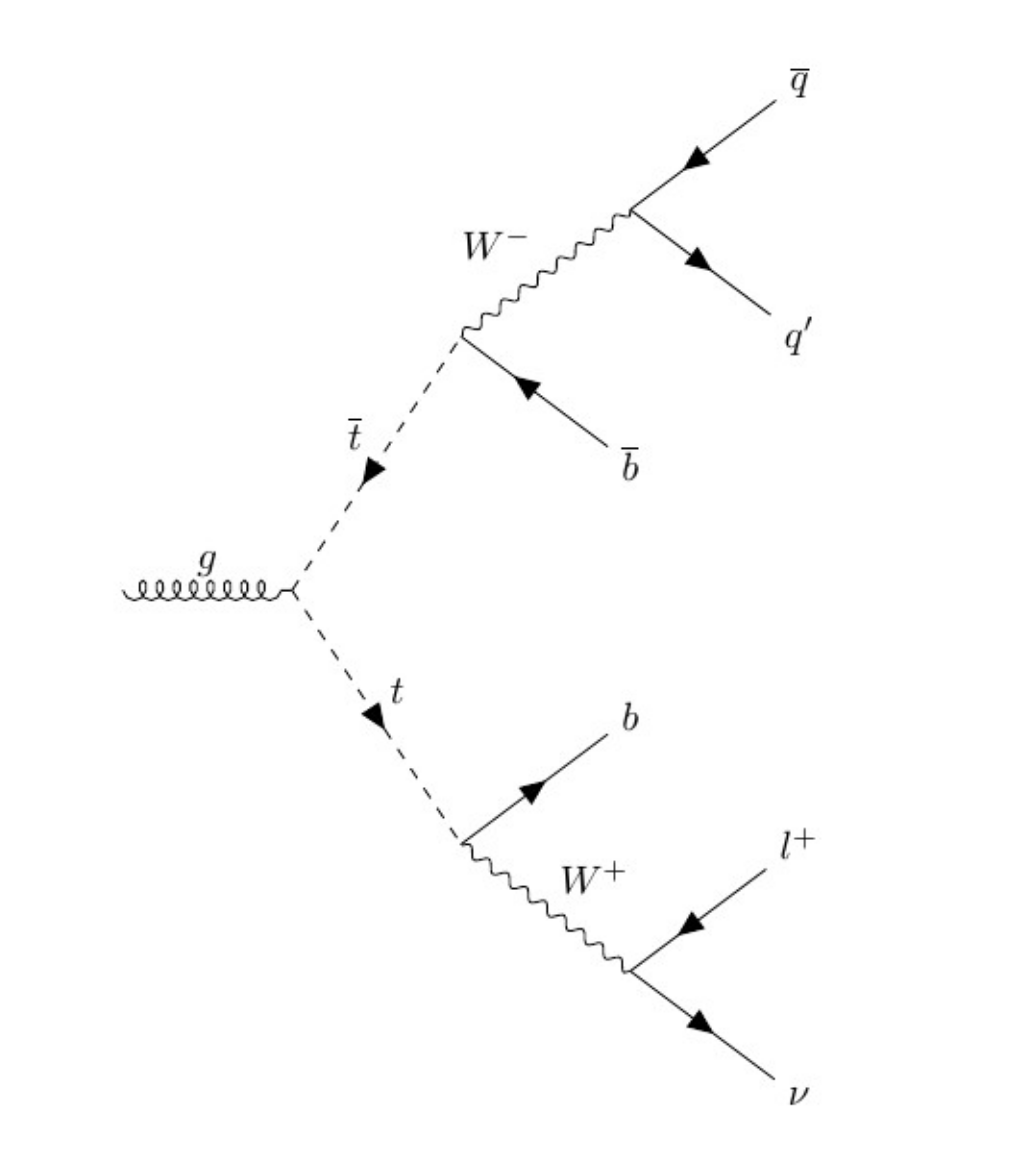
\includegraphics[height=6cm]{feynm_ttbar}
\caption{Feynman diagram for the $t \bar{t}$ decay}
\label{fig:feynmtop}
\end{figure}

The first analysis criteria takes into consideration that the lepton produced by the $t\bar{t}$ decay comes from the subsequent decay of a $W^+$ boson, as shown in Fig. \ref{fig:feynmtop}, meaning that their energy would be greater than $25 GeV$ in general. The decay of the $W^+$ boson also produces a neutrino, resulting in $\cancel{\it{E}}_{T} > 30$ GeV. The criteria for the four jets, including the lepton, assures a full reconstruction of the $t\bar{t}$ decay processes. There are also two b-tagged jets immediately produced by the $t\bar{t}$ decay as well as a pair of W bosons.\\

The $\cancel{\it{E}}_{T}$ of the $t\bar{t}$ decay was first modeled using the MC simulation method implementing the specified search criteria. This simulation was then plotted over the reconstructed data of the $t\bar{t}$ decay, as shown in Fig. \ref{fig:mtetop}. The simulation seems to correlate closely with the data, suggesting the simulation results are accurate in recreating expected scenarios.\\

%% WRITE ABOUT THAT
For this search a new variable called effective mass (${m}_{eff}$) was introduced since it might offer a parameter space in which the Z' signal can be distinguished from $t\bar{t}$ in Section 4.3. ${m}_{eff}$ was calculated using the equation:\\

\begin{equation}
{ m }_{ eff }\quad =\quad \sum { { p }_{ jets } } \quad +\quad { p }_{ l }\quad + \cancel{\it{E}}_{T}
\end{equation}

The effective mass of the $t\bar{t}$ decay is shown in Fig. \ref{fig:mefftop}. It shows a distinct peak at $\sim$200 GeV and has a large tail that flattens off at energies greater than 2500 GeV.

\begin{figure}[htbp]
  \begin{center}
    \mbox{
      \subfigure[Histogram of MET for the $t \bar{t}$ decay]{\scalebox{0.32}{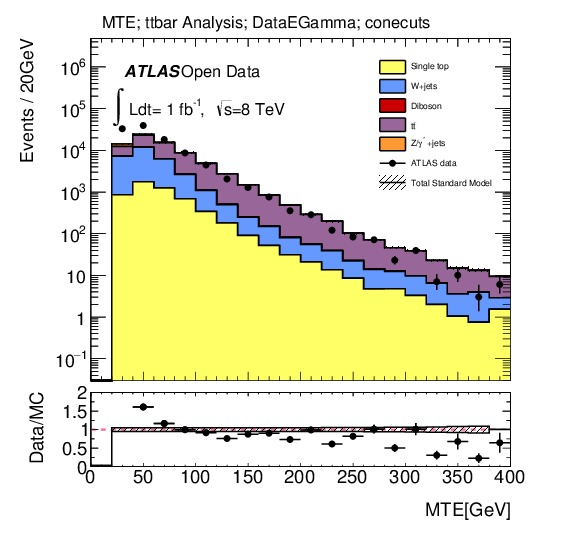
\includegraphics{ee_conecuts_mtetop_egamma}
\label{fig:mtetop}}} \quad
      \subfigure[${m}_{eff}$ histogram for the $t \bar{t}$ decay]{\scalebox{0.32}{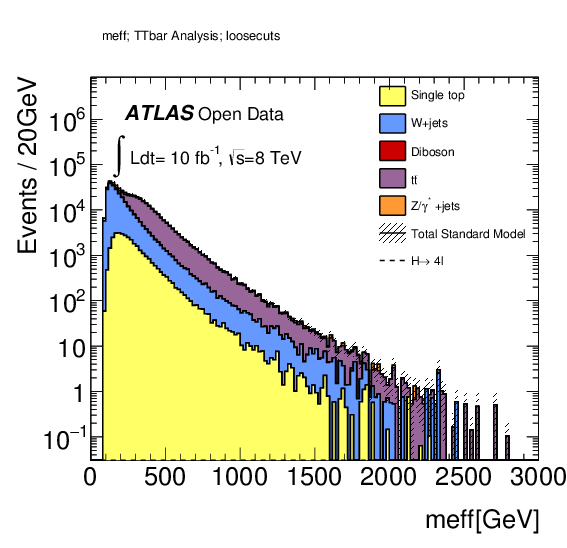
\includegraphics{ee_loosecuts_mefftop}\label{fig:mefftop}}}
      }
  \end{center}
\end{figure}

%% SAM END
\pagebreak
%% ANN START
\section{Results \& Discussion}
\subsection{Higgs Search - First Approach}
Two same flavour, opposite sign lepton pairs are selected, a lepton quadruplet, because they can form Higgs boson candidates \cite{atlas2014fiducial}. Furthermore, trigE (a trigger has fired in the egamma stream) and/or trigM (a trigger had fired in the muon stream) has to be true. The criteria for the ZZ analysis required the two Z bosons to be on-shell, however for finding the Higgs boson, one of them will be off-shell. This is because the mass of the Higgs is smaller than twice the Z mass, which requires one of the Zs to be off-shell.\\

\begin{figure}[htbp]
  \begin{center}
    \mbox{
      \subfigure[ZZ background processes and Higgs signal at 1 $\invfb$]{\scalebox{0.28}{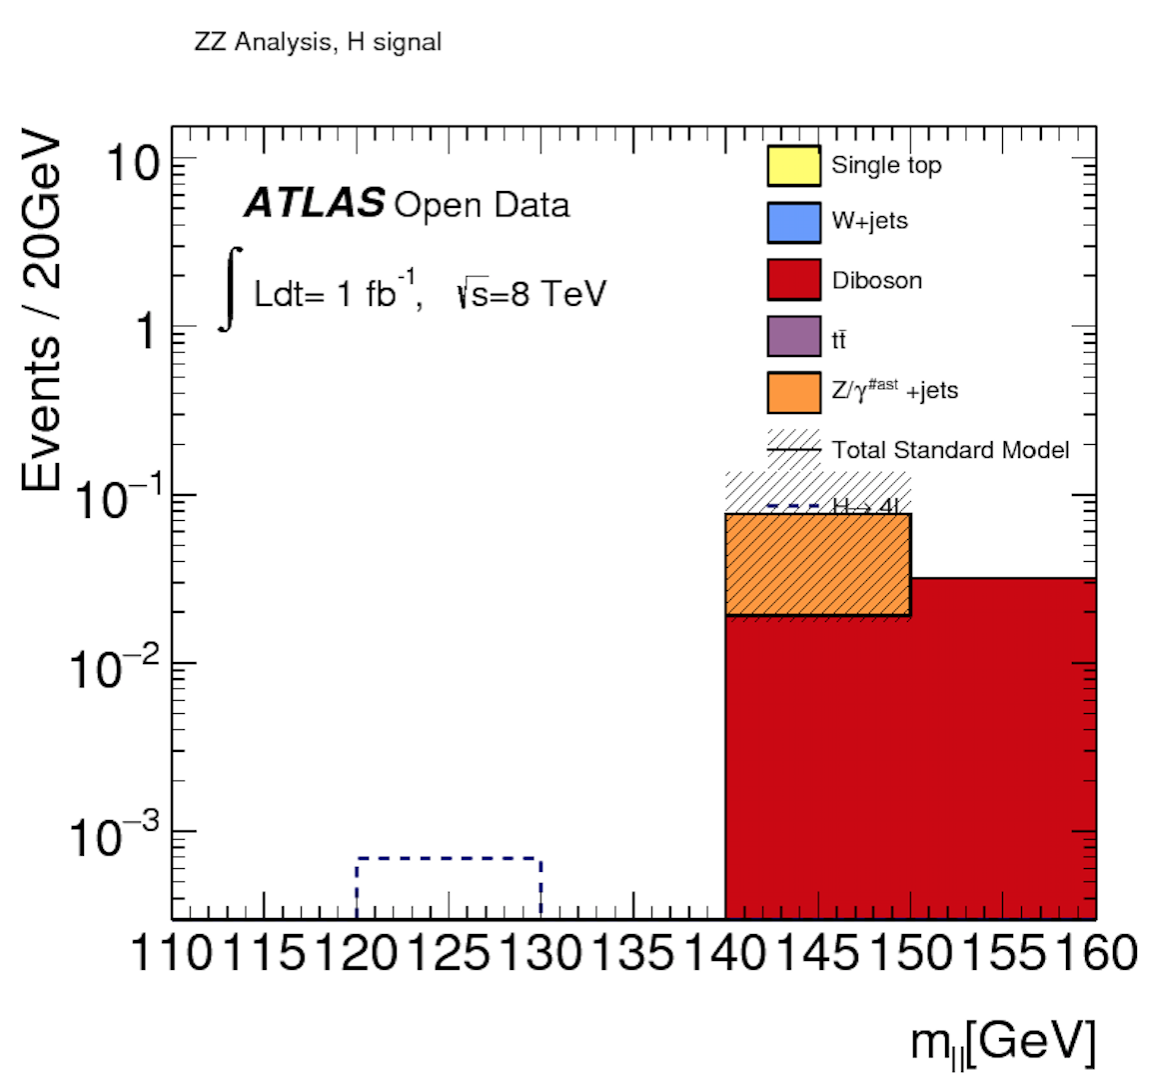
\includegraphics{IM_1fbar_ZZanalysis}
\label{fig:firsthiggs}}} \quad
      \subfigure[ZZ background \& Higgs signal at 1 $\invfb$ with $lep\_pt > 15$ GeV]{\scalebox{0.30}{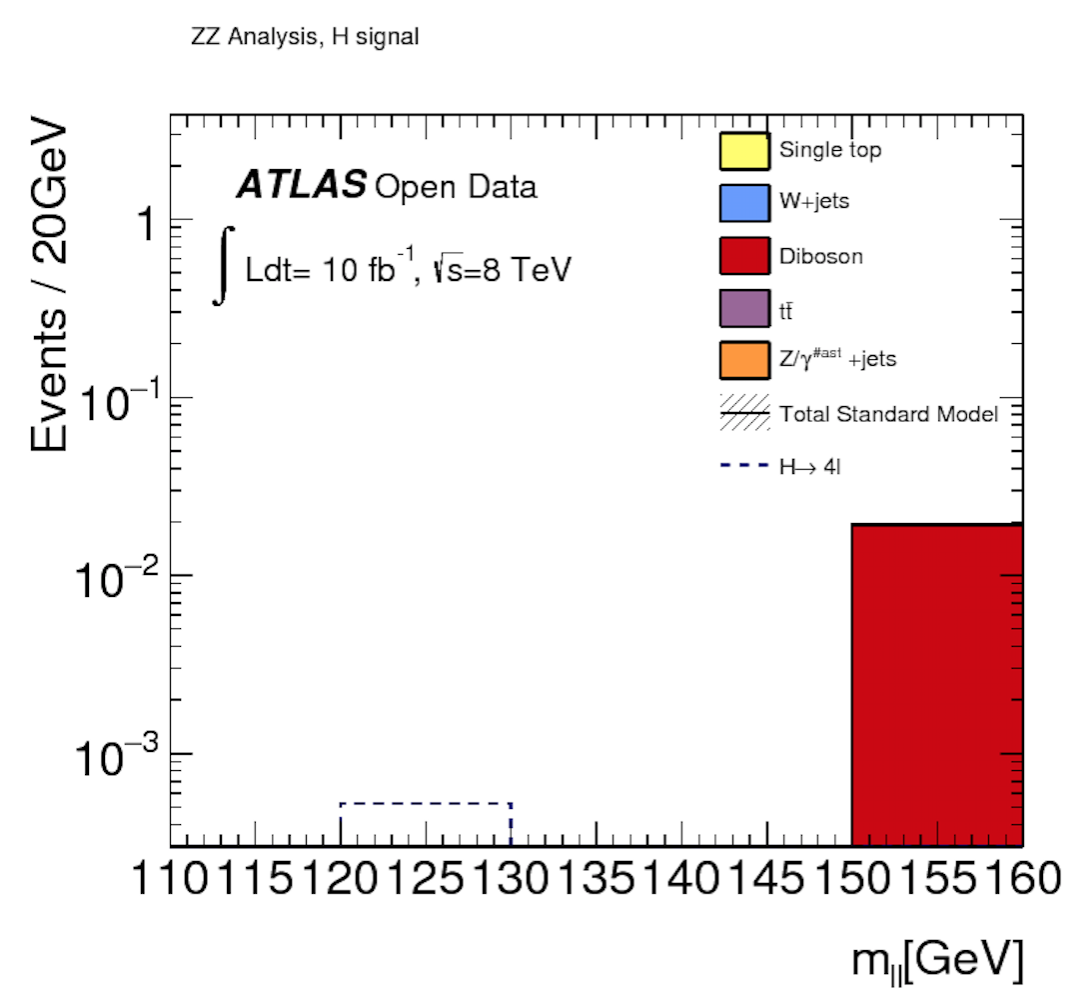
\includegraphics{higgs_fail}\label{fig:higgs_fail}}}
      }
  \end{center}
\end{figure}


Fig. \ref{fig:firsthiggs} shows a plot of all background processes for the ZZ analysis with a signal for Higgs. The standard deviation for the Higgs signal with 1 $\invfb$ is negligible. The main background process is diboson, so in order to get a significant signal for the Higgs boson the diboson background has to be suppressed. Moreover, a Z+jets background is visible. This background is removed by increasing the minimum $lep\_pt$ to 15 GeV instead of 10 GeV, see Fig. \ref{fig:higgs_fail}. However, the Higgs signal also decreased by applying this criteria. Since there is still no SM background at the invariant mass of the Higgs boson, it is not possible to calculate the $\sigma$ value of the signal.\\

When considering 120 to 130 GeV, the Higgs yield is equal to 0.00059 and the total SM background is zero. Therefore, the standard deviation for the Higgs boson cannot be calculated using Eq. 5, because it is not possible to divide by zero. Moreover, the signal is very small ($\sim$0.001) and will most likely not be significant.\\

As can be seen in Fig. \ref{fig:deltaphi1}, the azimuthal angular difference $\Delta \phi$ between the first two leptons of a diboson and Higgs decay are the same and both in the bin around zero. This implies that the leptons from the t$\bar{t}$ decay move parallel after the decay. However, since there is no difference between the ZZ and the Higgs decay, this property cannot be used to separate the signal from the background.\\

\begin{figure}[H]
\centering
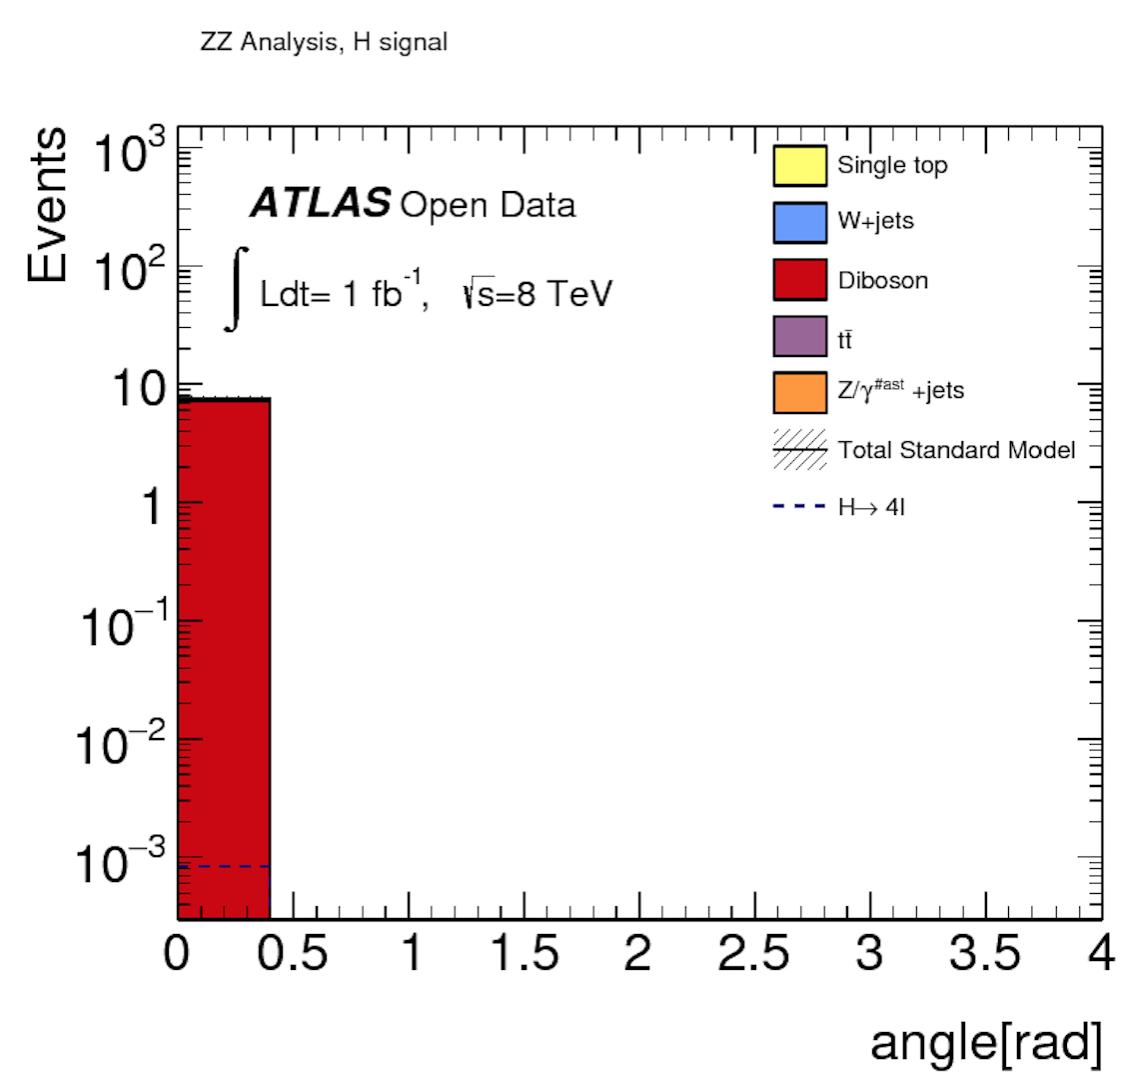
\includegraphics[height=6cm]{DeltaPhi1_screenshot}
\caption{Azimuthal angular difference $\Delta \phi$ between the first two leptons of ZZ and Higgs decay}
\label{fig:deltaphi1}
\end{figure}

\subsection{Higgs Search - Second Approach}
In order to be able to calculate the standard deviation of the Higgs boson, some background is needed as well as a signal. For these reasons, the cuts in the analysis were loosened. Most importantly, it was required to have four leptons in the final state, either electrons and/or muons. Furthermore, there must be at least one quadruplet (same flavour/opposite charge) present. The diagram in Fig. \ref{fig:loosesthiggs} was plotted for this analysis, using 10 $\invfb$ and including the background.\\

Figure \ref{fig:loosesthiggs} shows that the signal has a frequency of ~10 at 125 GeV and it becomes clear that these restrictions are not good enough to distinguish the Higgs signal from the background. Especially the Z+jets background is large, even though this cannot produce four leptons. It is likely that the jets resulting from the Z decay are falsely classified as leptons. The diboson background is as expected not very large, because this background peaks for invariant masses higher than 200 GeV (~220 GeV, see Fig. \ref{fig:invmzz}). \\

\begin{figure}[H]
\centering
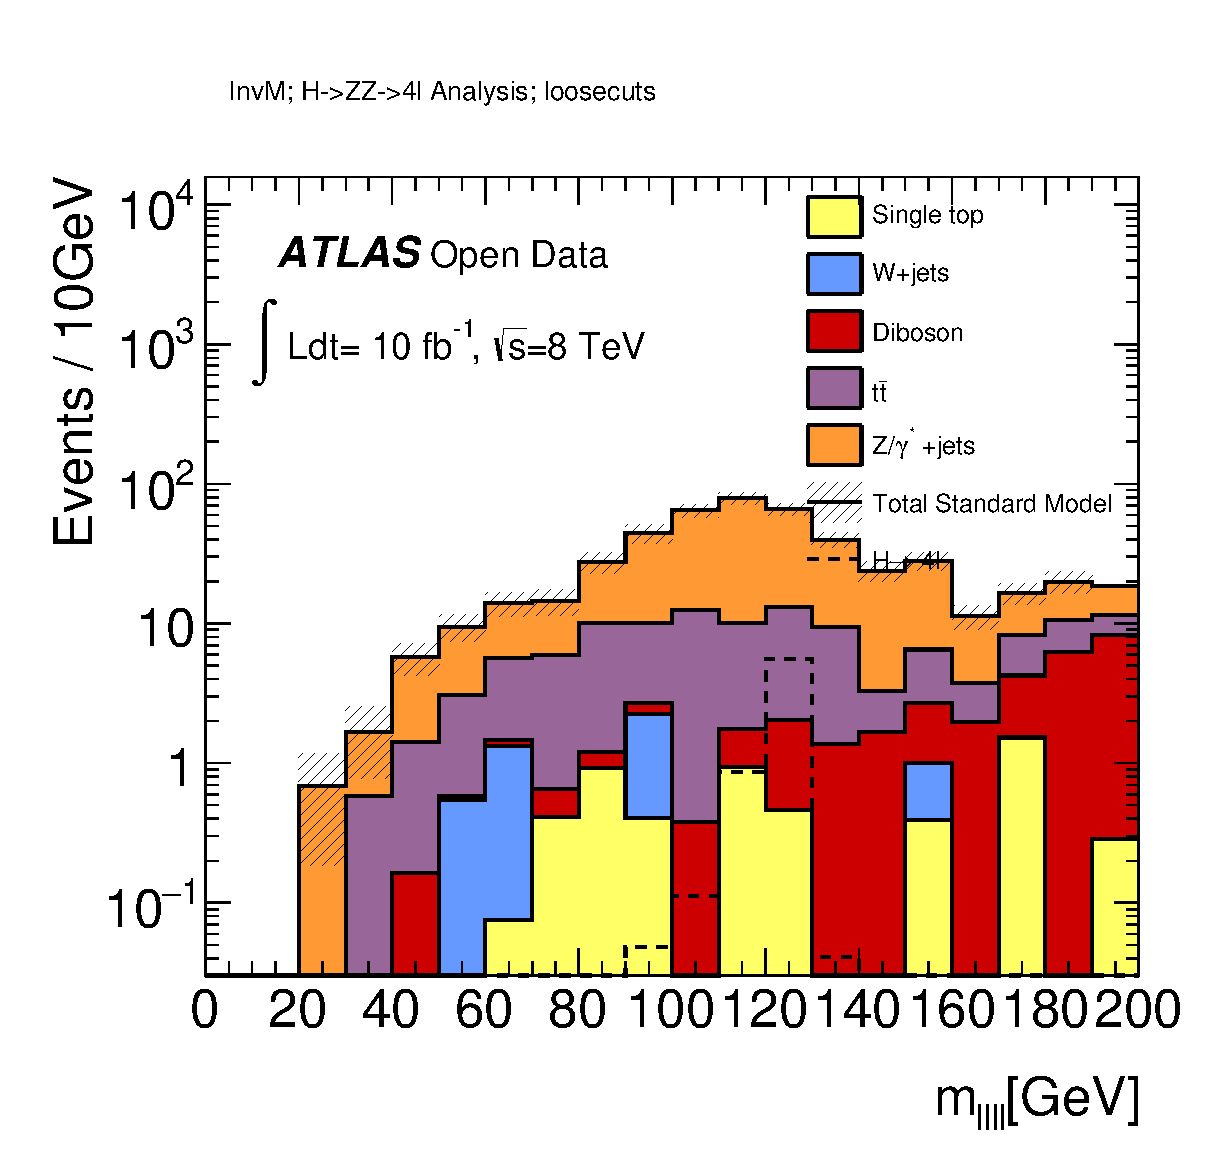
\includegraphics[height=6cm]{higgs_loosest_invm}
\caption{4 required leptons; Higgs signal and background at 10 $\invfb$}
\label{fig:loosesthiggs}
\end{figure}

To decrease the background without cutting the signal, the most on-shell Z boson was required to be within 20 GeV of the mass of the Z boson. This cuts all background under 80 GeV as can be seen in Fig. \ref{fig:20fromz}.\\

When the range 110 to 130 GeV is taken into account the $\sigma$ value for the Higgs signal is equal to 0.43. Further cuts on the invariant mass of the other dilepton pair were made to decrease some of the Z+jets and other backgrounds. When the invariant mass of this dilepton pair was required to be greater than 20 GeV, the low mass resonances were cut out and a lot of the Z+jets background was reduced (see Fig. \ref{fig:m3420}).\\

Finally, if the leptons are required to be isolated the significance for the Higgs boson increases a lot when considering the range from 120 to 130 GeV. The isolation of leptons is necessary, because it excludes most of the ‘fake’ leptons. The isolation makes sure only the leptons without surrounding transverse momenta or energy are considered, therefore only clean data is counted. This results in a standard deviation of $\sigma = 2.23$ for 10 $\invfb$. Increasing the luminosity, resulted in the $\sigma$ values listed in Table 1 below. For a significance greater than 5, a luminosity of at least \lumi $= 50.5 \invfb$ are needed. This result is plotted in Fig. \ref{fig:finalhiggs}.
\begin{table}[h]
\centering
\caption{Sigma values for different luminosities}
\label{my-label}
\begin{tabular}{|c|c|c|c|c|c|c|c}
\hline
\lumi           & 1 \invfb & 10 \invfb & 20 \invfb & 30 \invfb & 40 \invfb & 50\invfb & 50.5 \\ \hline
120 - 130 GeV & 0.70     &   2.23       &     3.15      &       3.86    &     4.46      &      4.98	&	5.01     \\ \hline
\end{tabular}
\end{table}
\begin{figure}[htbp]
  \begin{center}
    \mbox{
      \subfigure[4 leptons + 20 GeV deviation from true Z mass; Higgs signal and background at 10 $\invfb$]{\scalebox{0.3}{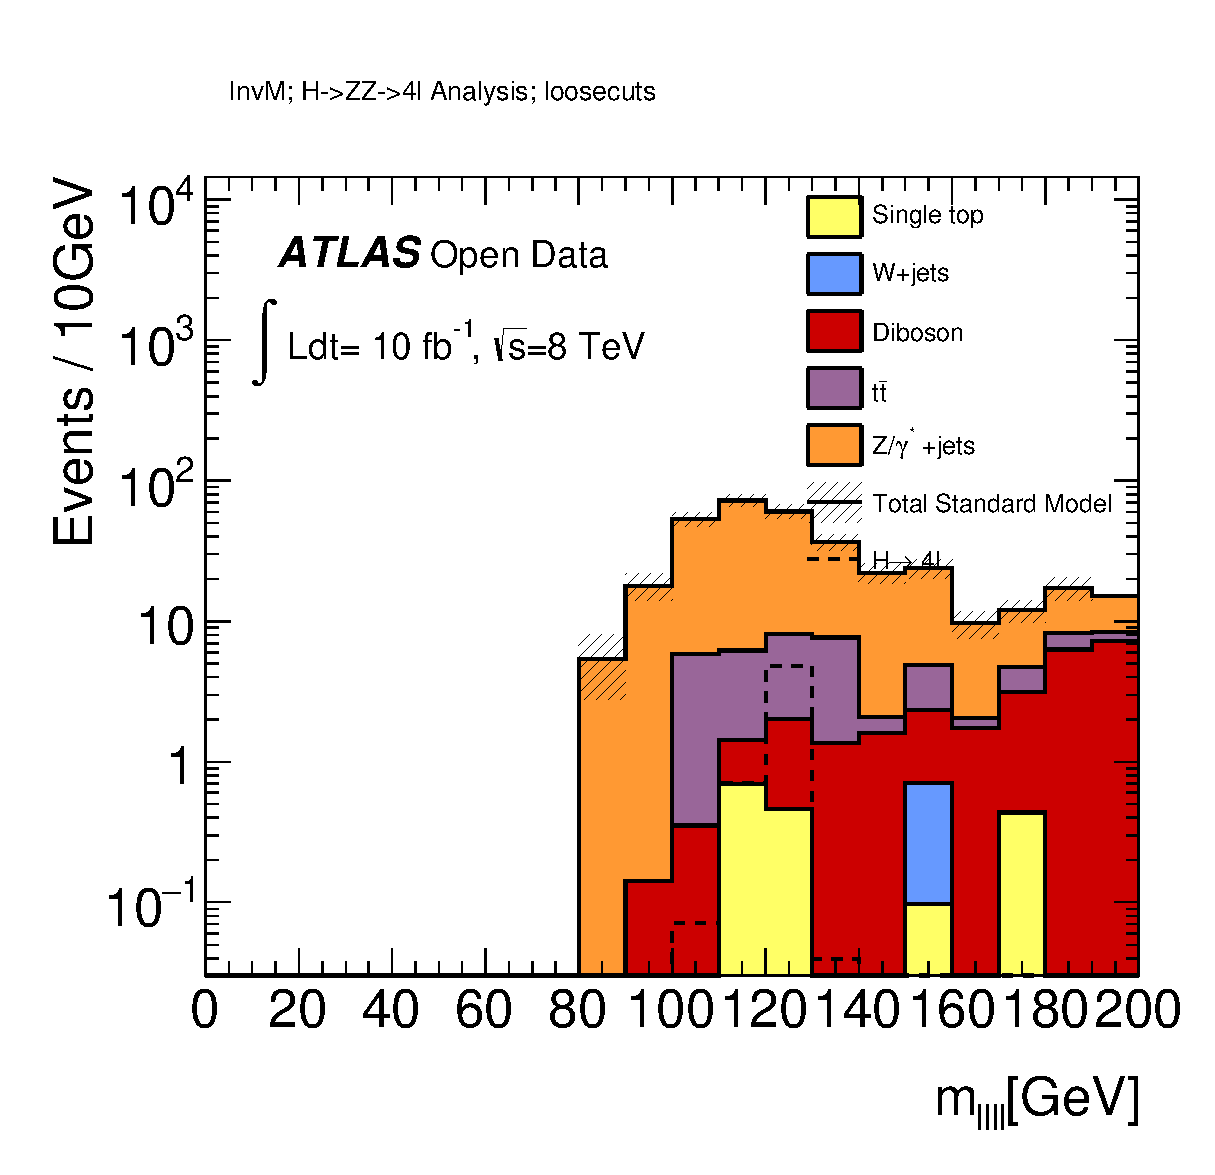
\includegraphics{higgs_20fromZwith10fb}
\label{fig:20fromz}}} \quad
      \subfigure[4 l + 20 GeV Z deviation + invariant mass of dilepton pair $>$ 20 GeV; Higgs signal and background at 10 $\invfb$]{\scalebox{0.30}{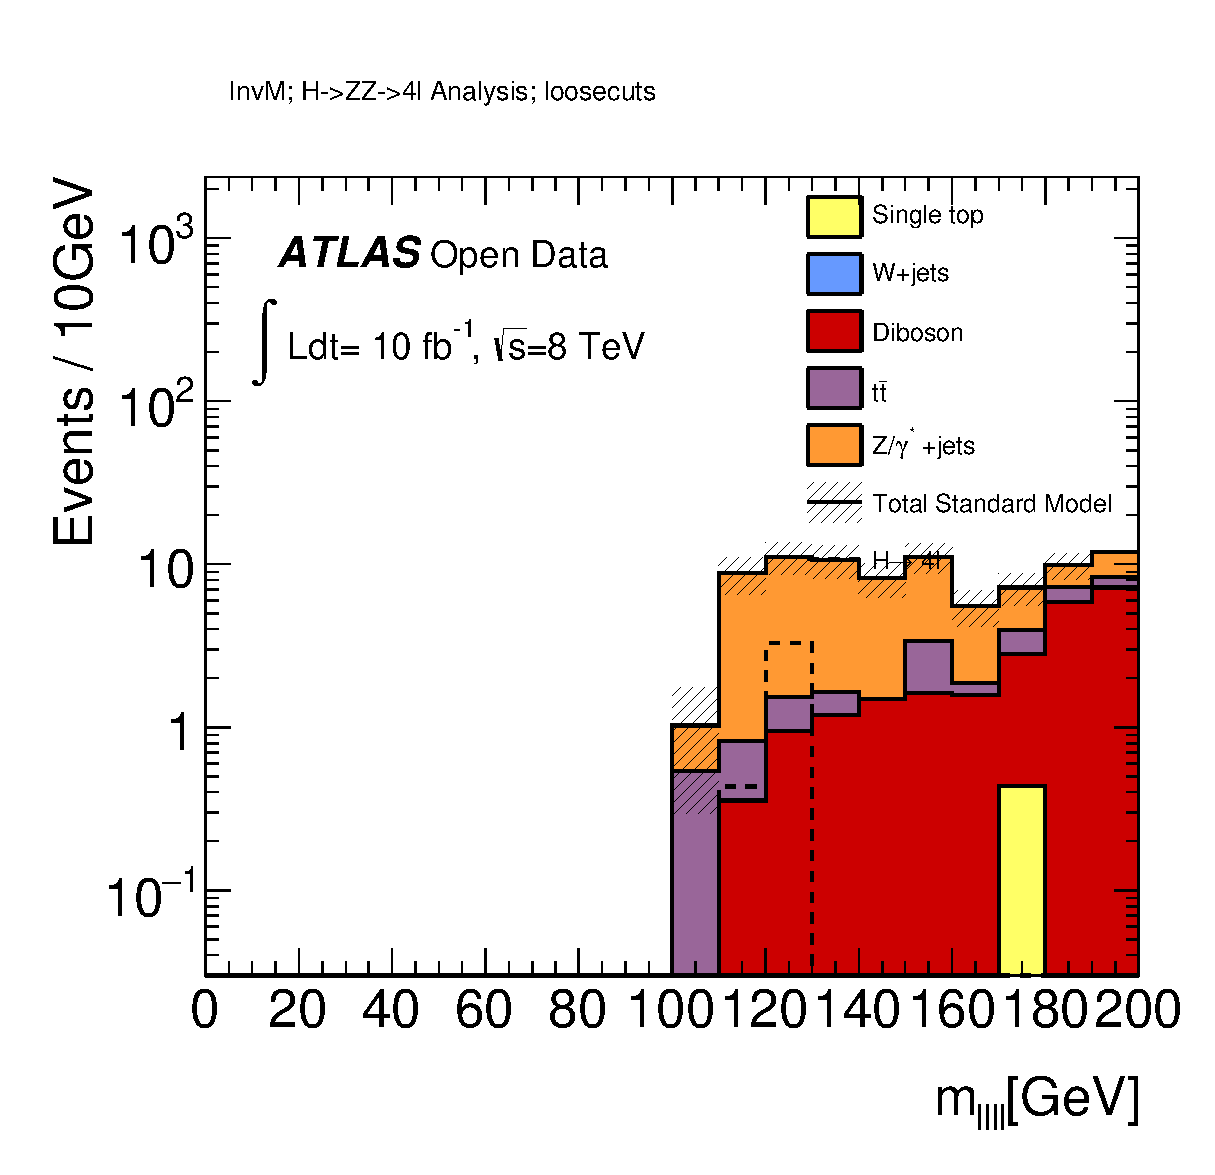
\includegraphics{higgs_m34_20}\label{fig:m3420}}}
      }
  \end{center}
\end{figure}
\begin{figure}[H]
\centering
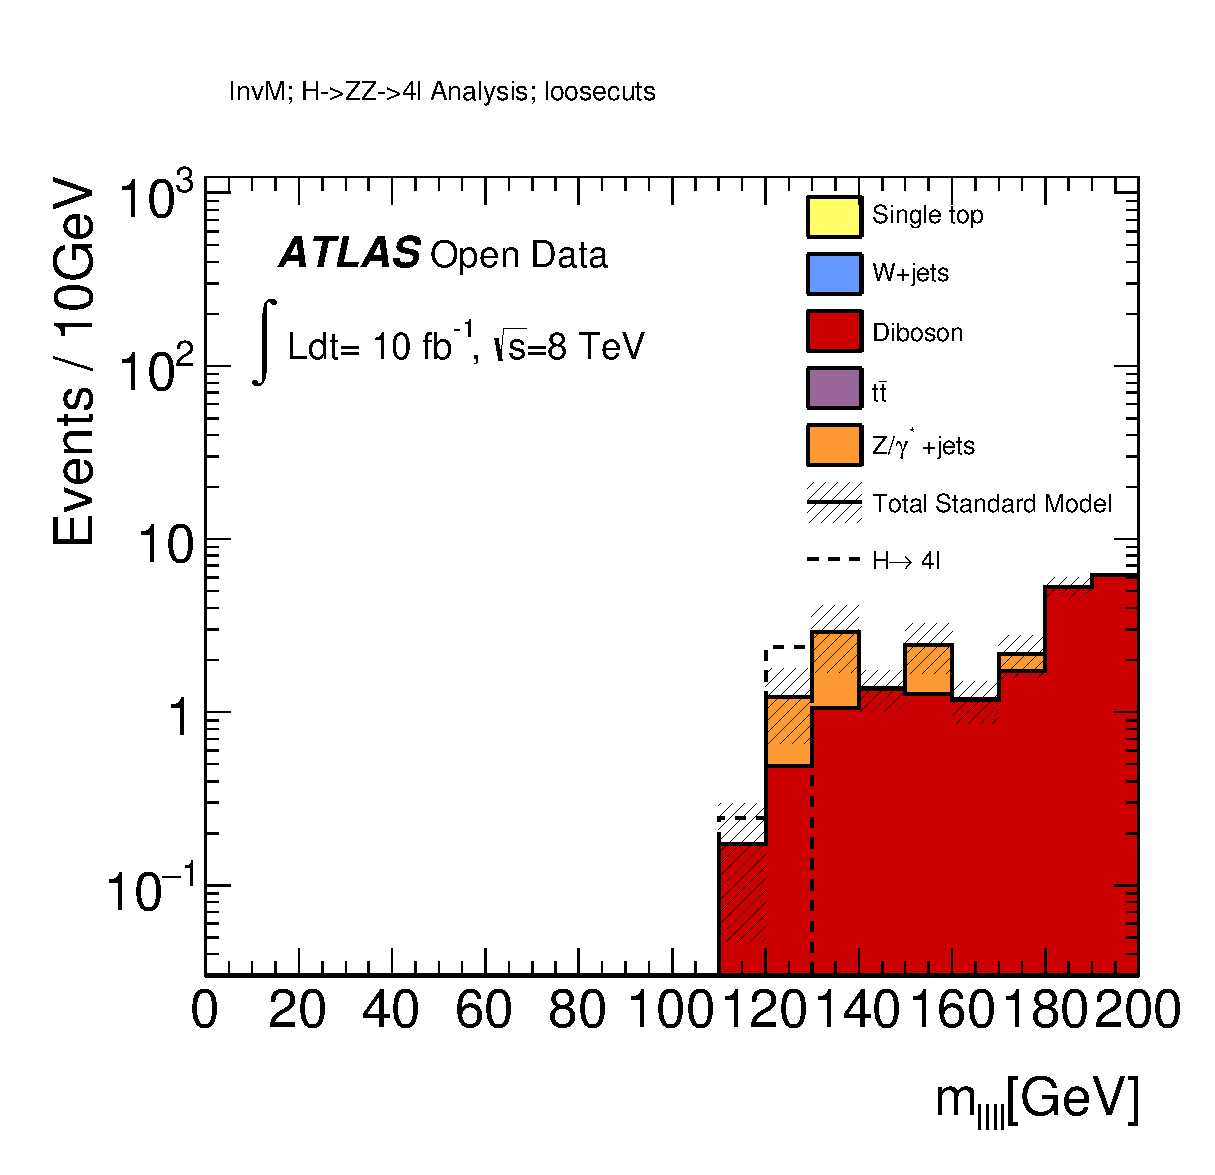
\includegraphics[height=6cm]{higgs_m34conefinal}
\caption{Histogram of the effective mass for the $t \bar{t}$ decay}
\label{fig:finalhiggs}
\end{figure}
%% ANN END
%% MARK START
\subsection{Z' search}
The Z' is a new heavy vector boson predicted by many theories that are trying to extend the current SM such as the Sequential Standard Model (SSM) or the ${E}_{6}$ Grand Unified Theory (GUT) model \cite{hayden2013z}. Based on these models the Z' is expected to have the same couplings as the lighter Z but with a much larger mass in the TeV region. The discovery of a new heavy vector boson is very likely to be one of the first signals for new physics at higher centre-of-mass energies at the LHC. This is due to the fact, that vector bosons generally have high branching fractions for clean decay modes, such as leptonic decays, and additionally tend to have higher cross-sections than other SM processes \cite{hayden2013z}.\\

Fig. \ref{fig:feynmzprime} shows the Z' decay diagrams which is considered for this search: first decay into a $t$$\overline t$ pair that then further decays into a $b$$\overline b$ pair and two W bosons. Subsequently one of the W bosons decays hadronically and the other leptonically.\\

In order to search the Z' in the semileptonic top pair channel the following search criteria were implemented:
\begin{itemize}
\item Exactly one lepton with ${p}_{T} > 25$ GeV
\item Minimum of four jets of which two have to be b-tagged
\item $\cancel{\it{E}}_{T} > 30$ GeV 
\item ${m}_{T}(W) + \cancel{\it{E}}_{T} > 30$ GeV
\end{itemize}

\begin{figure}[H]
\centering
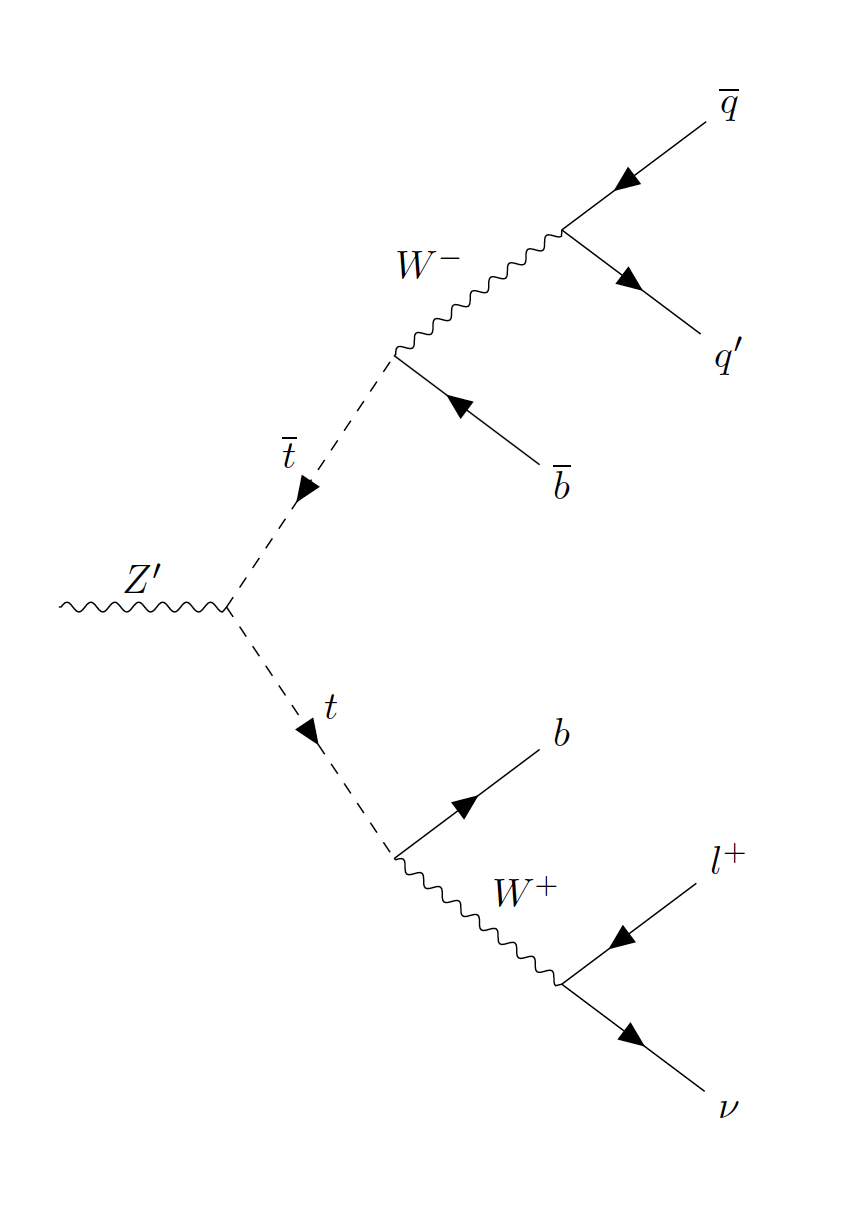
\includegraphics[height=5cm]{feynm_ZPrime}
\caption{Feynman diagram for Z' decay}
\label{fig:feynmzprime}
\end{figure}

As previously mentioned in Section 3.5, a new variable called effective mass (${m}_{eff}$, Eq. 7) was introduced for this search since it might offer a parameter space in which the Z' signal can be distinguished from the background. The obtained histograms for ${ m }_{ eff }$ are given for the range 2000-2300 GeV and 2300-2600 GeV in Fig. \ref{fig:meffzoomallzprime1fb2300} and \ref{fig:meffzoomallzprime1fb2600} respectively. All MC data sets with possible Z' masses were used together as signals on these plots and both plots were filled with the given data amount of 1 $\invfb$ but no signals were visible. In order to visualize potentially small Z' signals the luminosity was artificially scaled up to 10 $\invfb$ and the resulting plots are shown in Fig. \ref{fig:meffallzprime10fb2300} and \ref{fig:meffallzprime10fb2600}. It can be seen that the data scaling indeed revealed Z' signals which could not been spotted previously in Fig. \ref{fig:meffzoomallzprime1fb2300} and \ref{fig:meffzoomallzprime1fb2600}.\\

\begin{figure}[htbp]
  \begin{center}
    \mbox{
      \subfigure[2000-2300 GeV, 1 $\invfb$]{\scalebox{0.28}{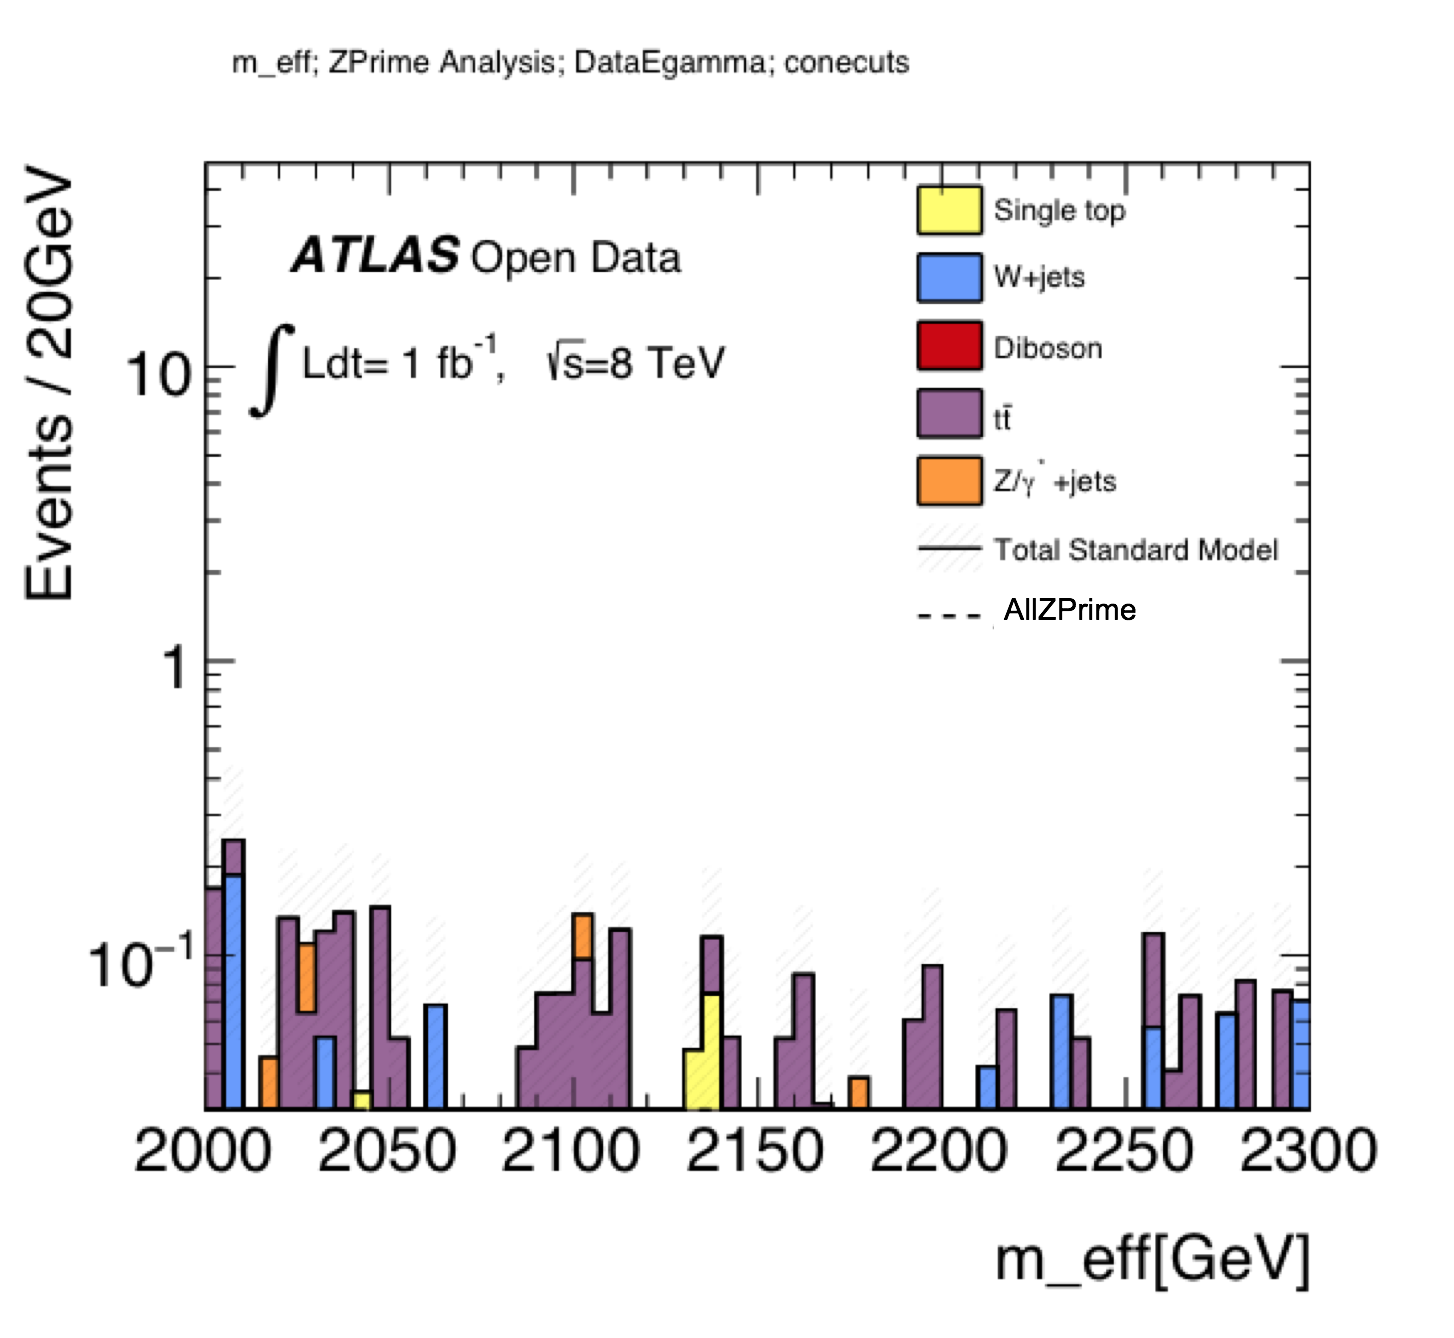
\includegraphics{ee_loosecuts_meff1_allzprime1fb20002300}\label{fig:meffzoomallzprime1fb2300}}} \quad
      \subfigure[2300-2600 GeV, 1 $\invfb$]{\scalebox{0.28}{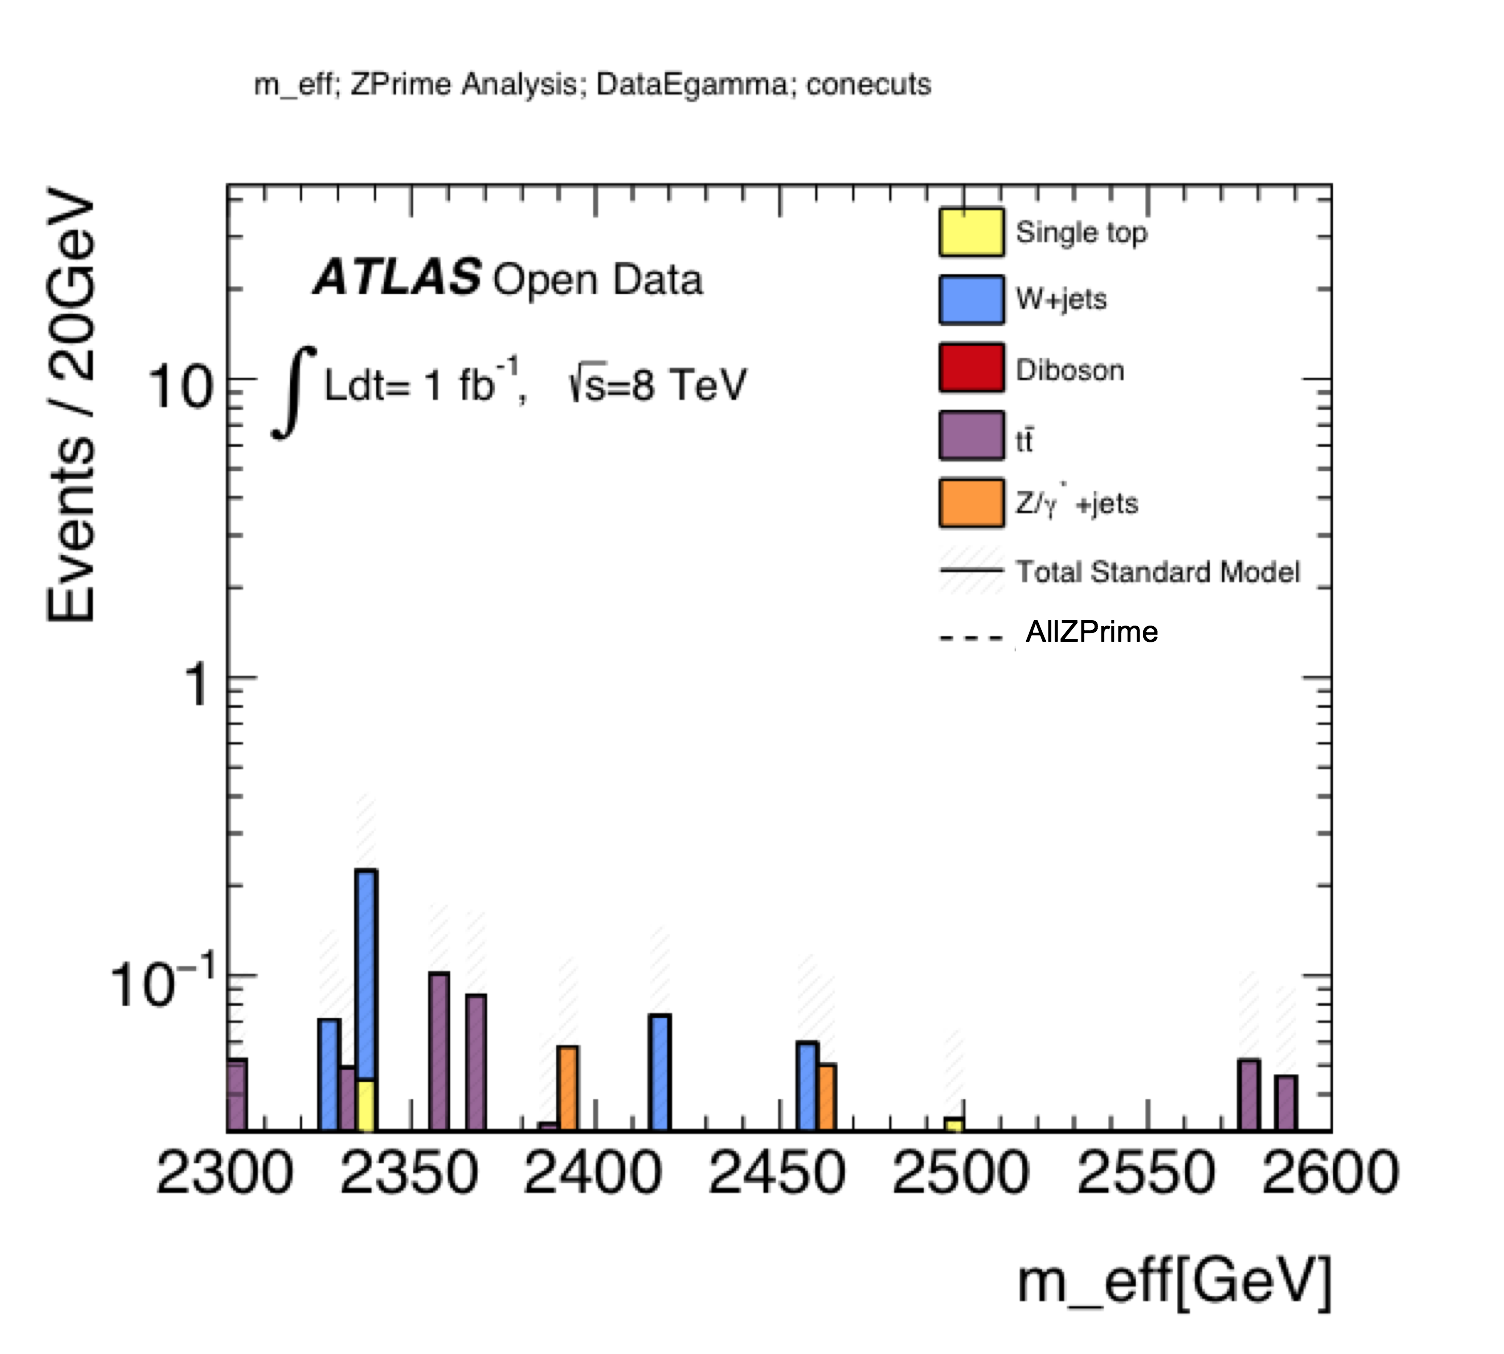
\includegraphics{ee_loosecuts_meff1_allzprime1fb23002600}\label{fig:meffzoomallzprime1fb2600}}}
      }
    \mbox{
      \subfigure[2000-2300 GeV, 10 $\invfb$]{\scalebox{0.28}{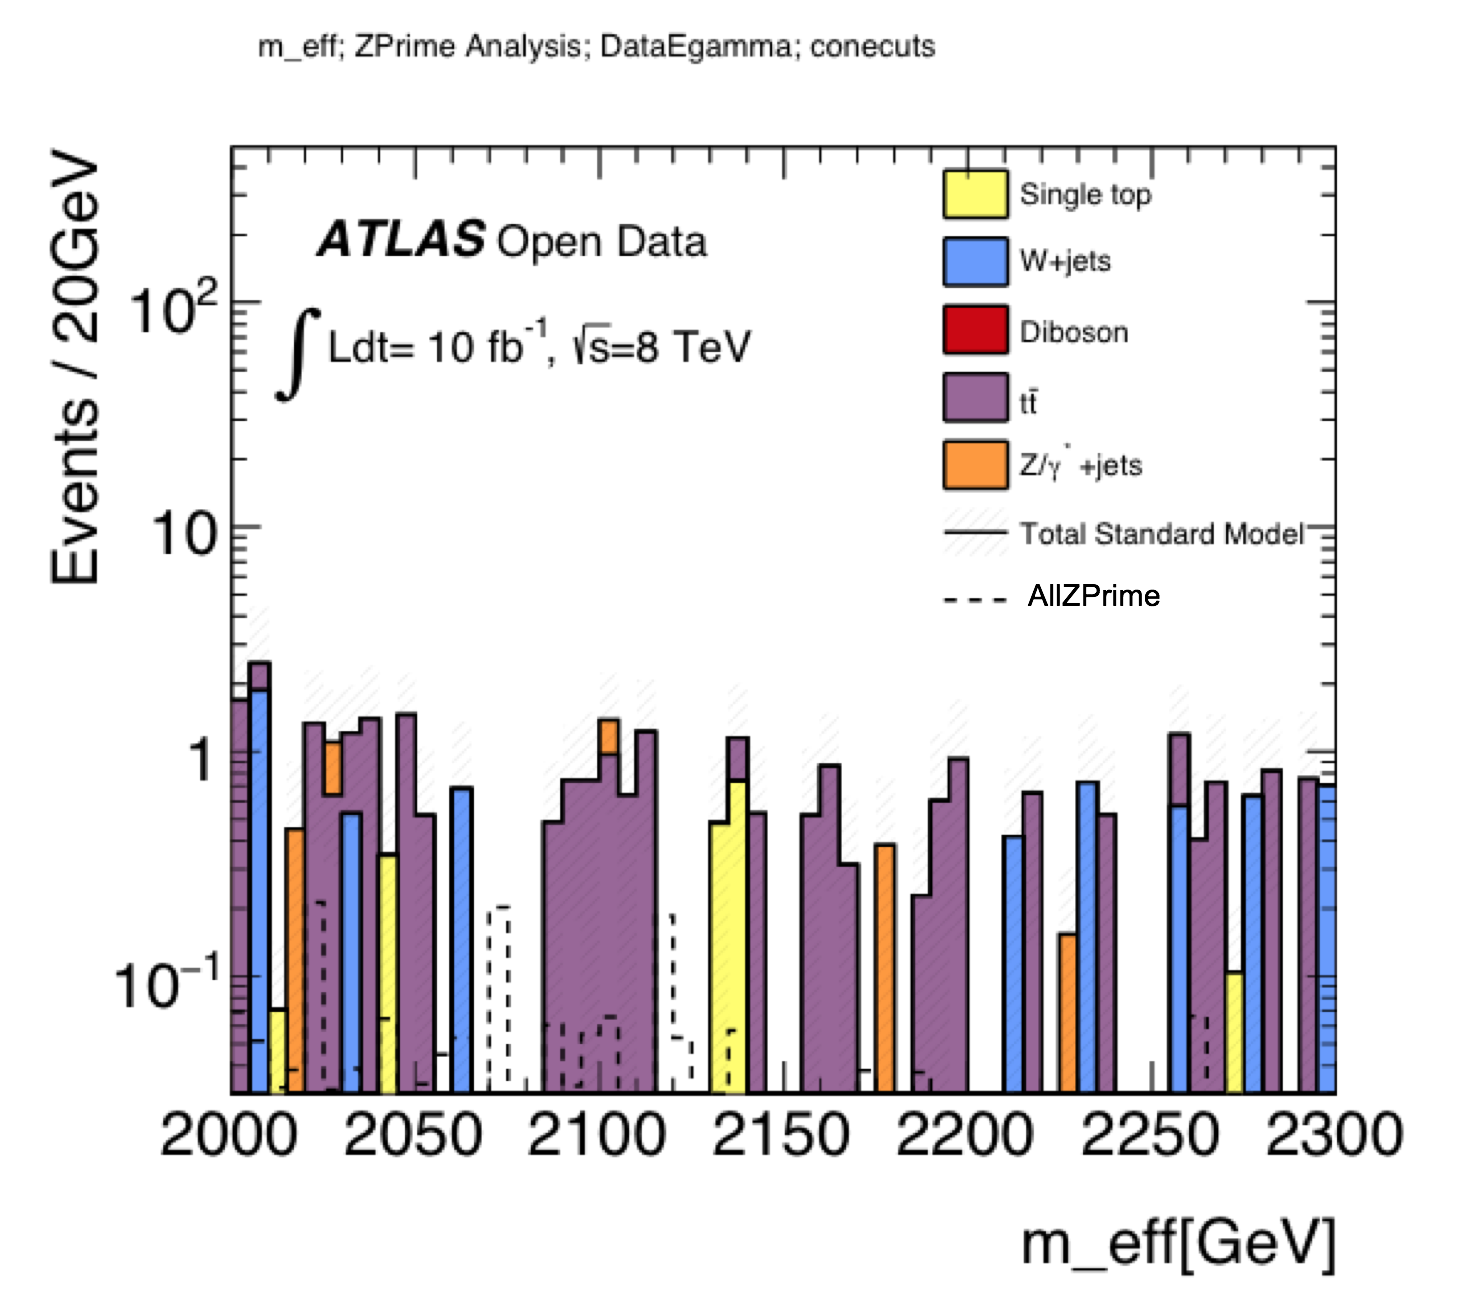
\includegraphics{ee_loosecuts_meff1_allzprimezooom20002300}\label{fig:meffallzprime10fb2300}}} \quad
      \subfigure[2300-2600 GeV, 10 $\invfb$]{\scalebox{0.28}{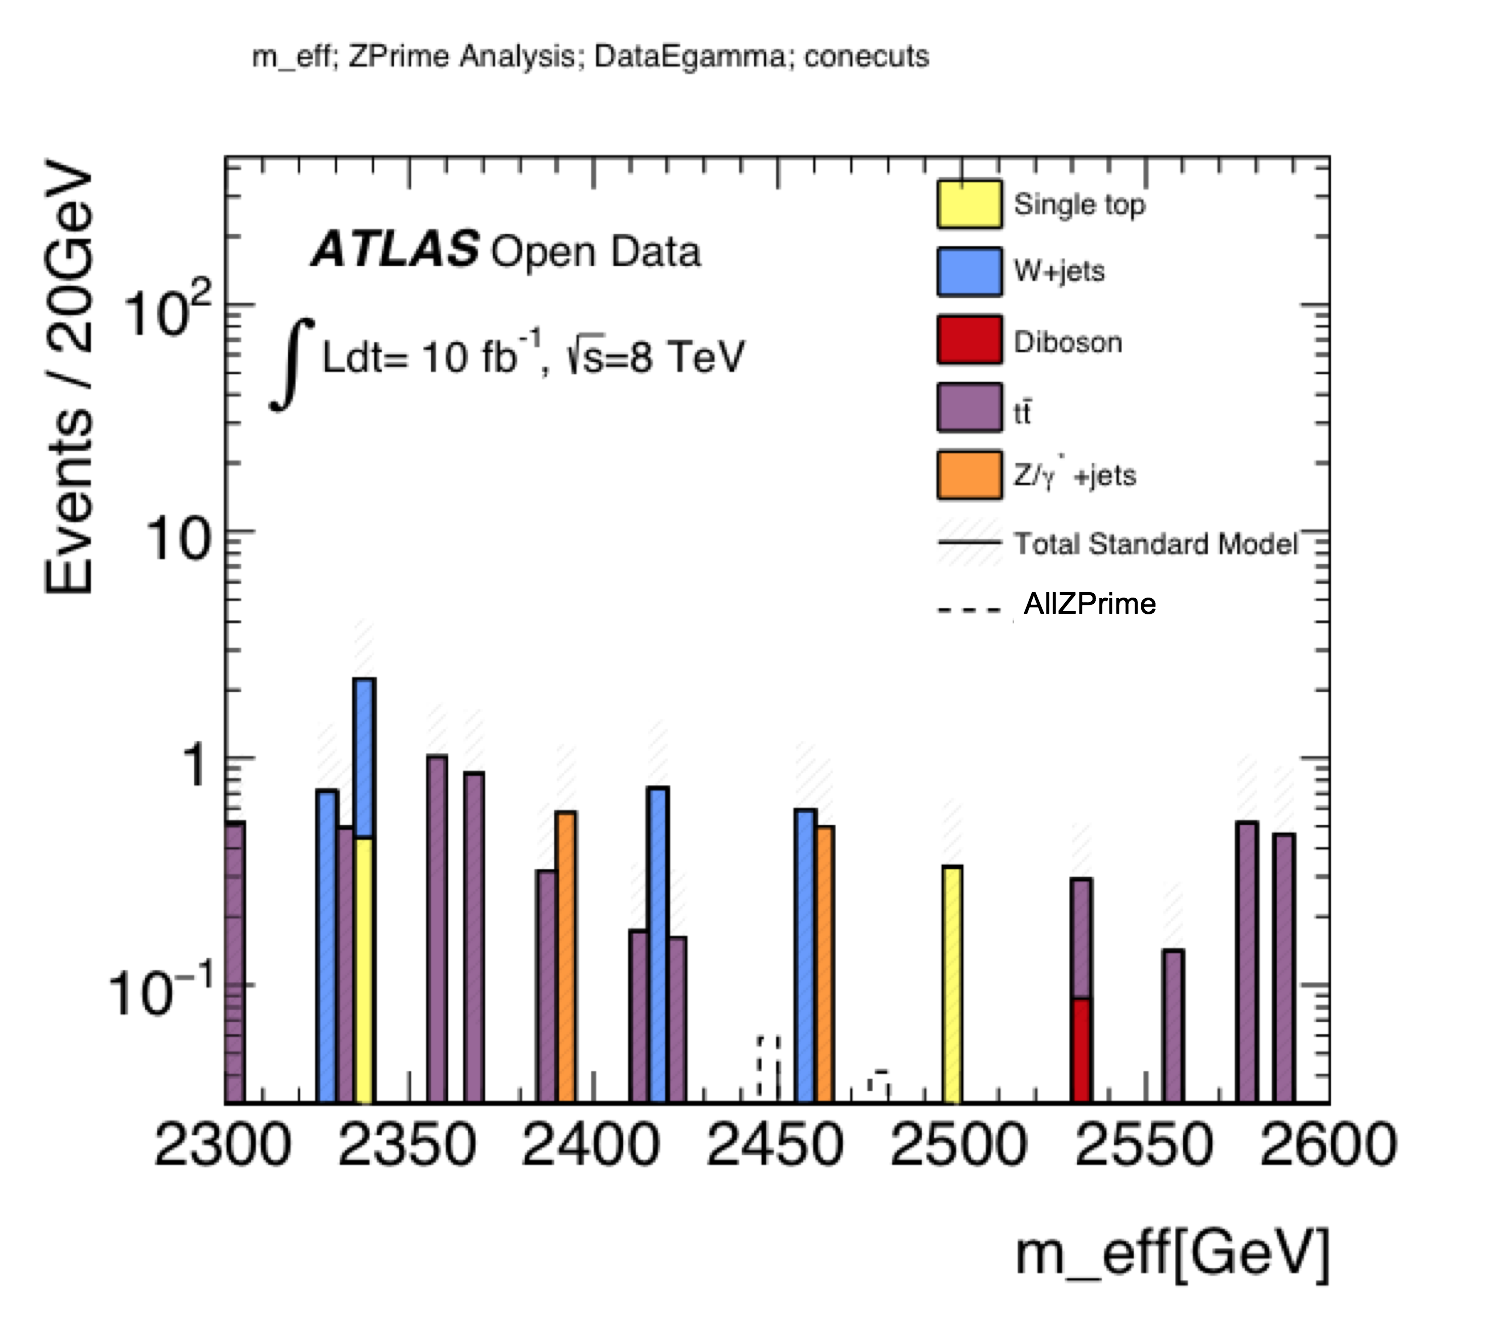
\includegraphics{ee_loosecuts_meff1_allzprimezoom23002600}\label{fig:meffallzprime10fb2600}}} 
      }
    \caption{${ m }_{ eff }$ histograms for Z' analysis with all possible Z' masses}
    \label{fig:my_car}
  \end{center}
\end{figure}

In order to calculate $\sigma$ values for these Z' signals more subplots were plotted with increased number of bins. Only in the subplot from 2000-2150 GeV, demonstrated in Fig. \ref{fig:meffzoomallzprime}, several distinct signal regions that stand out from the background were found. However, since in the previous plots all Z' data sets were plotted together as signal it is impossible to determine which Z' mass candidate is causing the signal. In order to resolve this, all possible Z' masses were individually considered as signals and plotted between 2000 and 2150 GeV. The MC data sets for the Z' masses 400, 500, 1000, 1250, 1500, 1750, 2000, 2250, 2500 and 3000 GeV did not results in any signal peaks. However, when plotting the Z' mass of 750 GeV several signal peaks became visible as demonstrated in Fig. \ref{fig:meffzoom750zprime}.\\

\begin{figure}[htbp]
  \begin{center}
    \mbox{
      \subfigure[All possible Z' masses]{\scalebox{0.24}{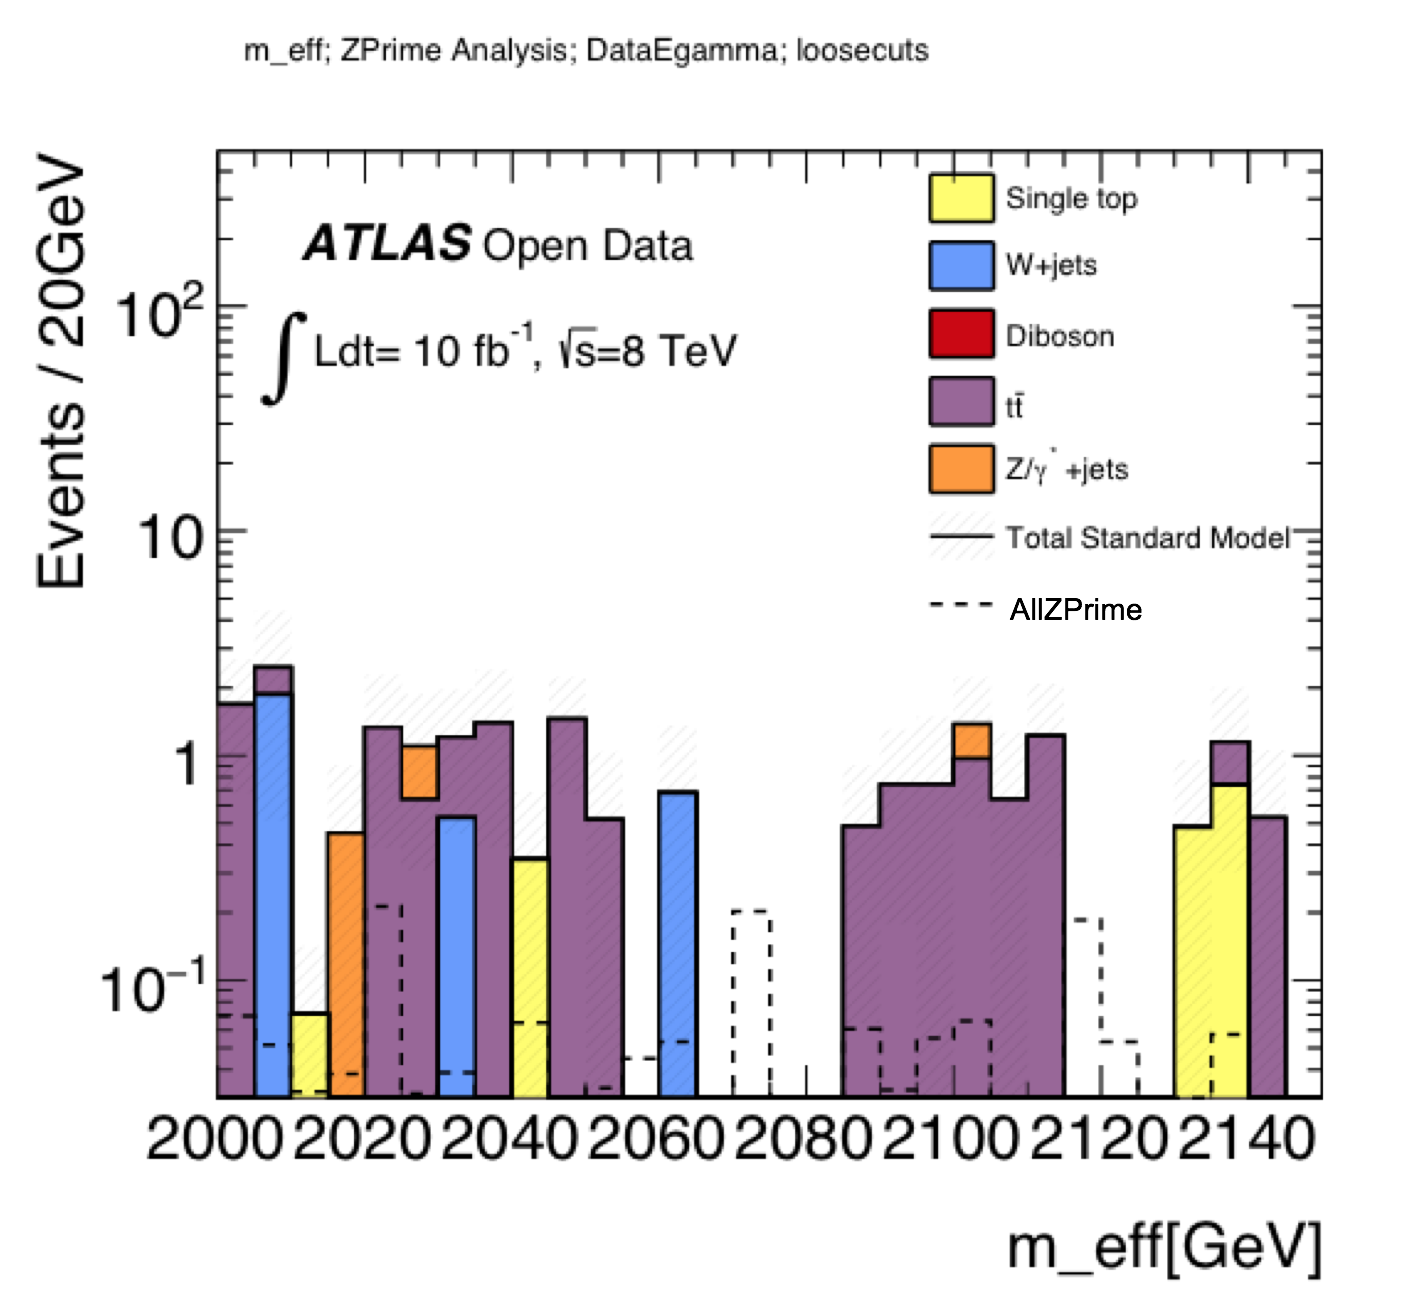
\includegraphics{ee_loosecuts_meff1_allzprime20002150}
\label{fig:meffzoomallzprime}}} \quad
      \subfigure[Assumed Z' mass of 750 GeV]{\scalebox{0.3}{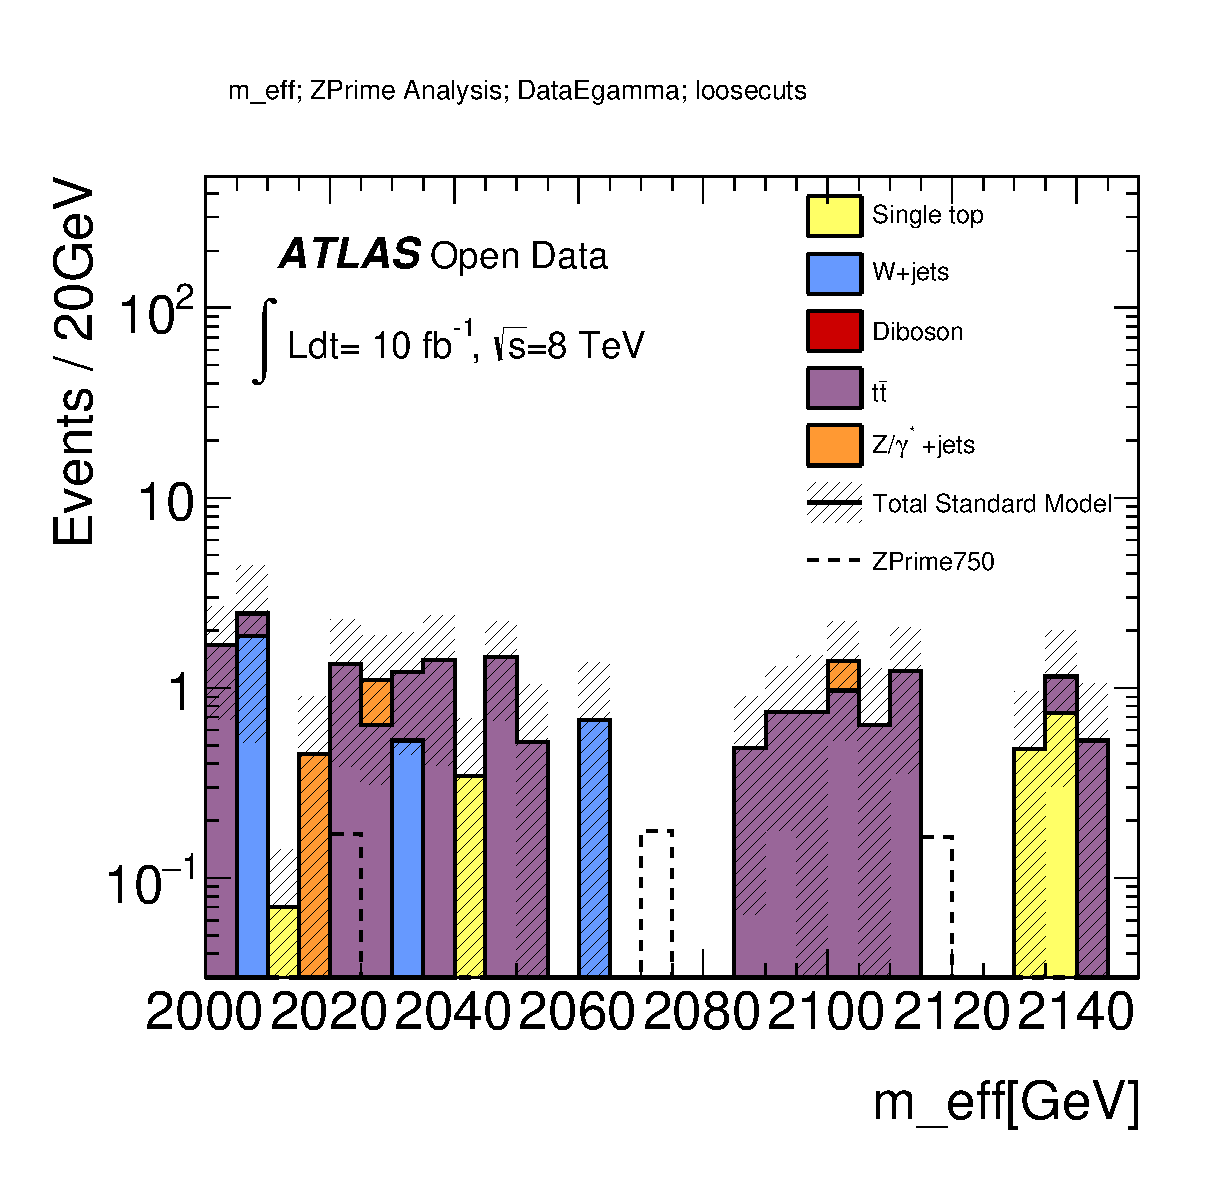
\includegraphics{ee_loosecuts_meff1_zoom750}\label{fig:meffzoom750zprime}}}
      }
    \caption{Enlarged signal regions in ${m}_{eff}$ histograms for Z' analysis with artificial 10 \invfb data}
    \label{fig:finalzprimesignals}
  \end{center}
\end{figure}

The statistical significance of the individual signal regions were analysed by computing the $\sigma$ values for varying bin ranges. Unfortunately, this was not possible for the signal in bin 24 since there is no SM background such that $\sigma = { S }/{ \sqrt { B }  }$ could not be calculated without division by zero. This, however, was possible for the signal in bin 15 because a very small SM background was present. The $\sigma$ values were calculated for the actual luminosity of 1$\invfb$ and for projected luminosities of 15, 20, 30 and 34$\invfb$. This statistical analysis revealed that a 5$\sigma$ discovery could only be achieved with a projected luminosity of \lumi = 34$\invfb$.

\begin{table}[h]
\centering
\caption{My caption}
\label{my-label}
\begin{tabular}{|c|c|c|c|c|c|}
\hline
Z' mass         & 750 GeV  & 750 GeV   & 750 GeV   & 750 GeV   & 750 GeV   \\ \hline
\lumi           & 1 \invfb & 15 \invfb & 20 \invfb & 30 \invfb & 34 \invfb \\ \hline
bin 14 - bin 15 & 2.73     & 3.35      & 3.87      & 4.73      & 5.04      \\ \hline
\end{tabular}
\end{table}


According to theory the Z' boson is predicted to be a heavy spin-1 vector boson. The spin of the boson can be measured by considering the angle between the b-tagged jets in the Z' decay process. In order to produce a spin-1 Z' boson, two heads on colliding protons must have their spins aligned in the same direction such that their half-integer spins add up to one. Thereafter, the angular momentum of 1 has to be conserved by all the subsequent decay products which most often manifests itself in the two b quarks travelling either in opposite or same direction. Hence, $cos(\Delta \phi)$ is expected to be dominant at -1 and +1 \cite{quantumdiaries}. Since the ATLAS detector measures the azimuthal angle $\phi$ of each jet, the angular difference $\Delta \phi$ between the two b-tagged jets and its cosine can be calculated according to the equation:\\

\begin{equation}
cos(\Delta \phi )\quad =\quad cos(\quad { { |\phi  }_{ jet\quad 1 }^{ b-tagged }\quad -\quad { \phi  }_{ jet\quad 2 }^{ b-tagged } }|\quad )
\end{equation}

The resulting histogram is shown in Fig. \ref{fig:cosphizprime} and the signal, consisting of all possible Z' masses, indeed has peaks at -1 and +1. This provides evidence that the Z' boson is indeed a spin-1 boson as predicted by the theory.\\

\begin{figure}[htbp]
  \begin{center}
    \mbox{
      \subfigure[Background with \lumi = 1 $\invfb$]{\scalebox{0.3}{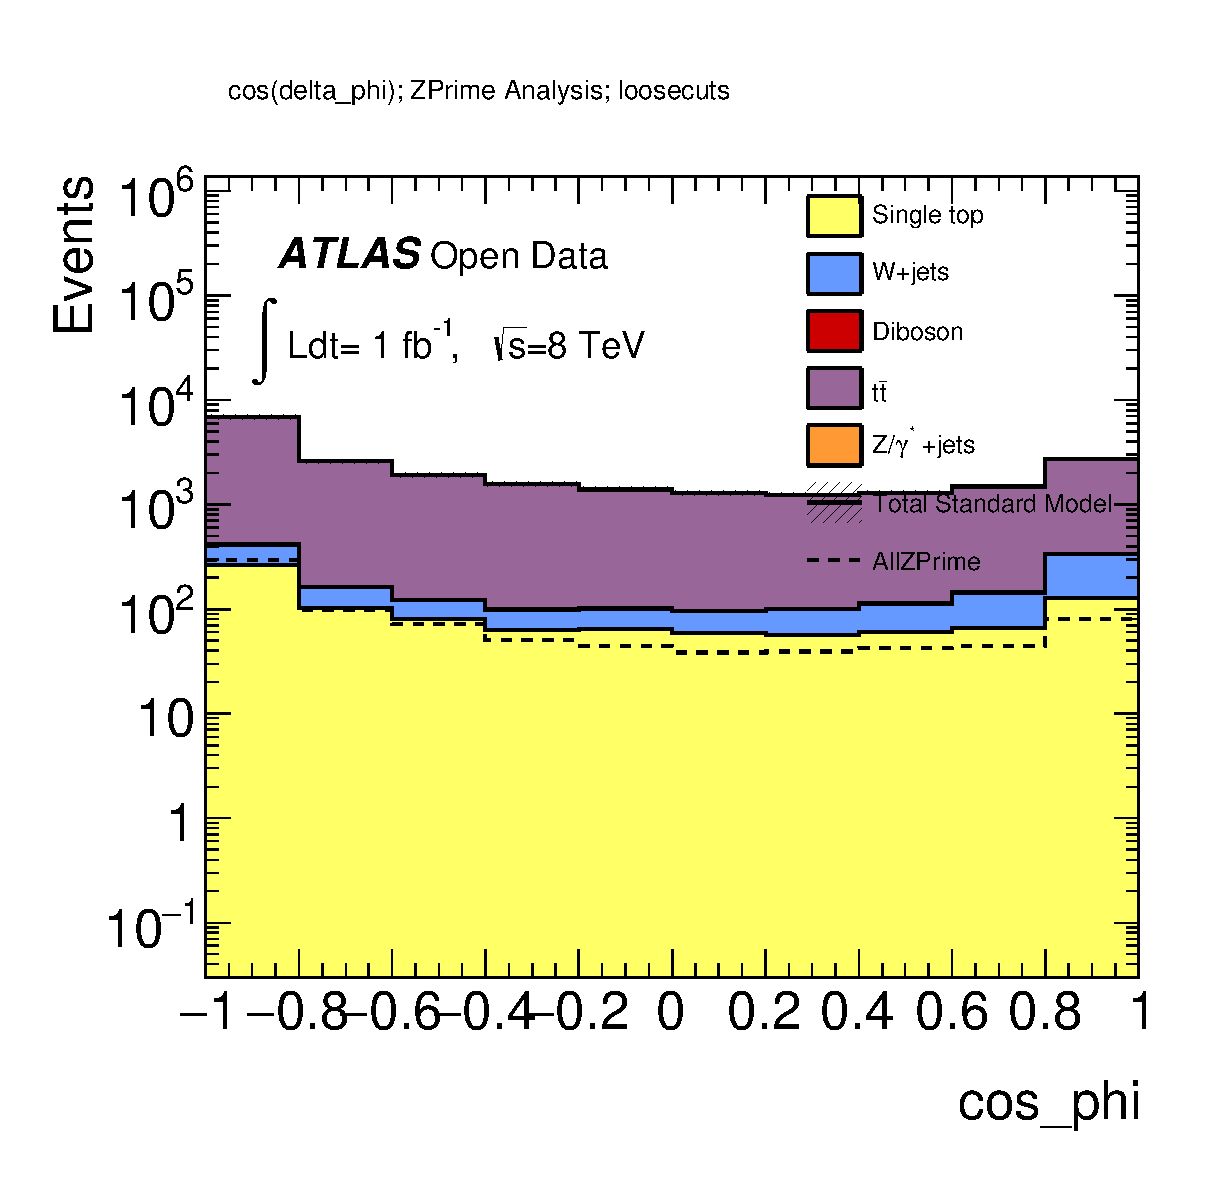
\includegraphics{ee_loosecuts_cosphi}\label{fig:cosphizprime}}} \quad
      \subfigure[Signal only with \lumi = 10 $\invfb$]{\scalebox{0.3}{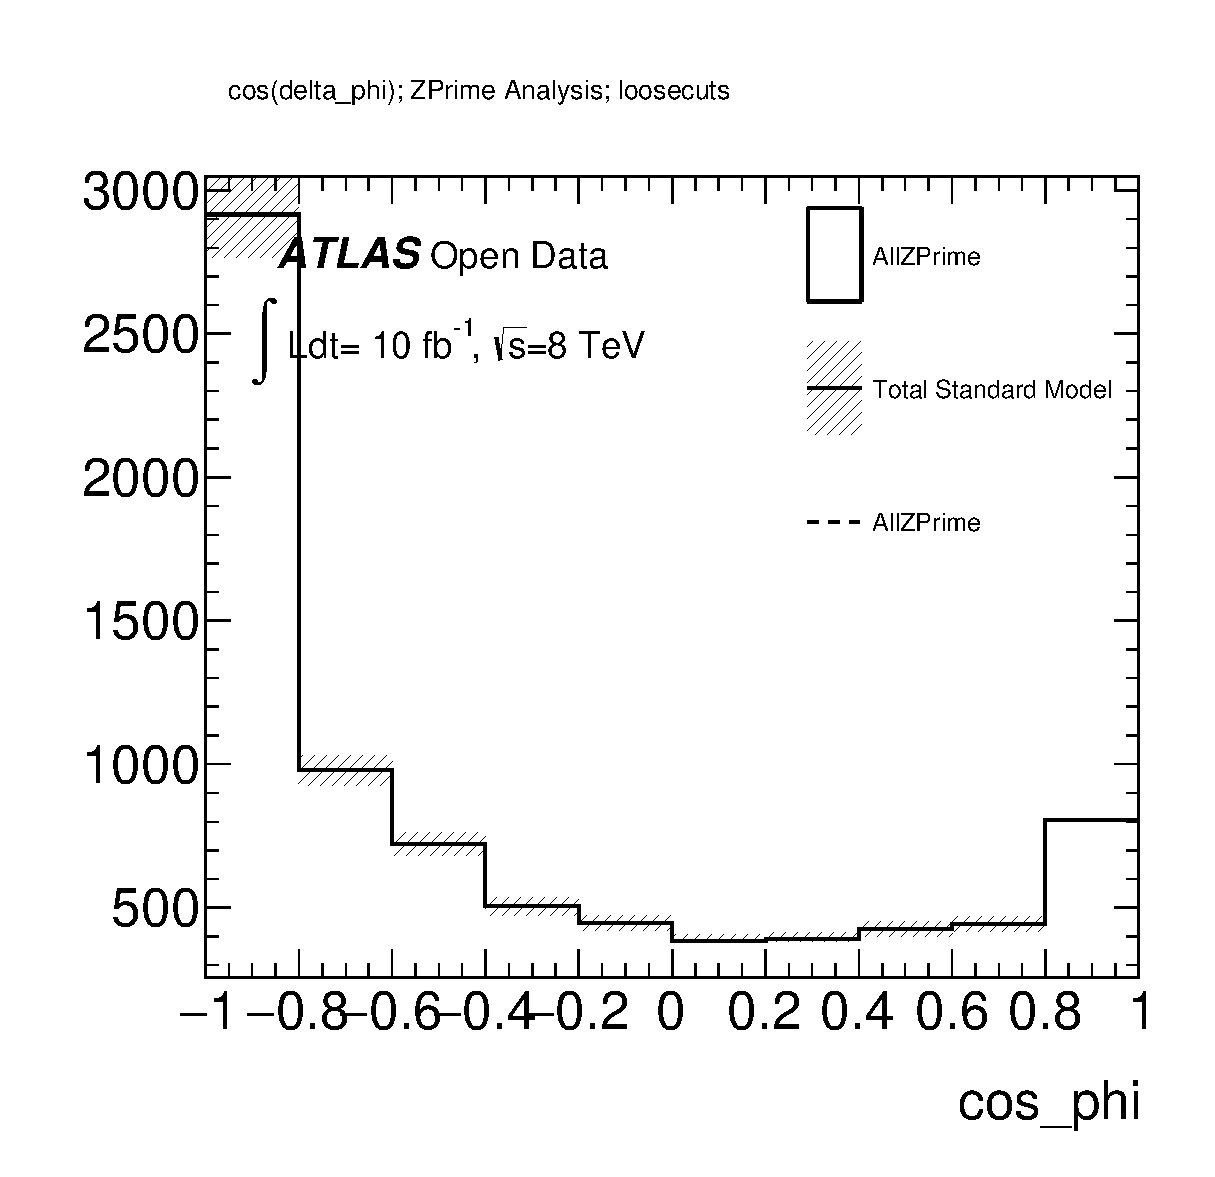
\includegraphics{ee_loosecuts_cosphi_zonly}\label{fig:cosphizprimezonly}}}
      }
    \caption{cos($\Delta \phi$) between the two b-tagged jets}
    \label{fig:my_car}
  \end{center}
\end{figure}

%% MARK END

\section{Conclusion}

In this report a collection of 1 $\invfb$ of run I ATLAS data from 2012 was used to analyse the main background processes for Higgs and Z' decay. By applying appropriate cuts the background was suppressed in order to increase the standard deviation of the signal from the background. \\

For the Higgs search, the main background processes were found to be diboson and Z+jets decays. The signal was found in the region between 120 and 130 GeV in the invariant mass histogram. According to the performed analysis a total of \lumi = 50.5 $\invfb$ is required for a statistically significant difference of 5 $\sigma$.\\

In the Z' decay, t$\bar{t}$, single top, W+jets and Z+jets decays were found to be the main background processes. The signal for the assumed Z' mass of 750 GeV was the only MC data set that yielded a signal outside of the background region. By considering the variable ${m}_{eff}$ the signal could be sufficiently separated from the background and with a projected \lumi = 34 $\invfb$ a statistical significance of 5 $\sigma$ could be achieved in the future.\\

In conclusion, even though the background was suppressed as much as possible by changing the search criteria appropriately, 1 $\invfb$ is by far not enough data to make a statistically significant discovery. More recent data from run II with $\sqrt {s} = 13$ TeV and run I data with higher luminosity should be considered for future research.\\

\bibliographystyle{apacite}
\bibliography{report}

\pagebreak
\section{Appendix}

\subsection{Code Template}
%% DHRUVA BEGIN
Most of the code produced are modifications to the original {\fontfamily{pcr}\selectfont TreeLooper.cxx} file, which runs the analysis. As such, most of the body of code is repeated among different analyses, with the only changes being within an iterative loop that runs over the data set. For the sake of brevity, we will present the body of code without the for loop in this section, and only the for loops for the analyses on the following pages.\\

\fontsize{7}{5}\selectfont
\begin{verbatim}
#define TreeLooper_cxx

#include "TCanvas.h"
#include "TreeLooper.h"
#include "TLeaf.h"
#include <TROOT.h>
#include <TChain.h>
#include <TSystem.h>
#include <TString.h>
#include <TFile.h>
#include <string>
#include <vector>
#include <iostream>
#include <fstream>
#include <sstream>

#include "TTree.h"
#include "TBranch.h"
#include "TVector.h"
#include "TH2I.h"
#include "TMath.h"
#include "TPaletteAxis.h"
#include <iomanip>
#include "TError.h"
#include "TLorentzVector.h"
//using namespace ROOT::Math;


using namespace std;

void TreeLooper::Loop(char* inputName, char* outputName)
{
	// The Begin() function is called at the start of the query.
	// When running with PROOF Begin() is only called on the client.
	// The tree argument is deprecated (on PROOF 0 is passed).

	string outputname="histos_";
	outputname.append(outputName);
	outputname.append(".root");

	std::cout<<"Set up output file to save histograms in"<<endl;
	f= new TFile(outputname.c_str(),"RECREATE");

	std::cout<<"Declare histograms"<<endl;
	setuphisto(m_myHisto1,"MyInvariantMassHisto",40,0.,400.); 
    // this is where we set up the histograms	
	setuphisto(m_myHisto2,"MissingTransverseEnergy",20,0.,400.);
	//the arguments are setuphisto(pointer, histogram name, 
    number of bins, lower X-value, upper x-value)
	setuphisto(m_myHisto3,"NumberOfJets",20,0.,20.);
    setuphisto(m_myHisto4,"Mt",40,0.,400.); // Mt graph	
	

	TChain::SetMaxTreeSize(19000000000);
	TTree::SetMaxTreeSize(19000000000);

	TChain *chain = new TChain("mini","");

	chain->Add(inputName);

	std::cout<<"Set up all branches in the tree"<<endl;
	Init(chain);

	Long64_t nentries = fChain->GetEntries();
	std::cout<<"number of entries in the tree= "<<nentries<<endl;
	
	


------------------------ANALYSIS GOES HERE------------------------





std::cout<<"done with looping, just need to save histograms"<<endl;
	
	f->Write();
	std::cout<<"Finished"<<endl;

}
void TreeLooper::setuphisto(TH1D*& histo, const char* name, int nbins,
double xlow, double xhigh){
	histo=new TH1D(name,name,nbins,xlow,xhigh);
	histo->Sumw2();
	histo->SetDirectory(f);
	std::cout<<"Registering histo... "<<name<<endl;
}


int main(int argc,char* argv[]) {
	if(argc!=0){
		std::cout<<"Running over file " <<argv[1]<<endl;
		if(argc==3){
		TreeLooper elephant;
		elephant.Loop(argv[1],argv[2]);
		}
	}
	return 0;
}
\end{verbatim}
%% DHRUVA END
\pagebreak
\subsection{WZ analysis}

\fontsize{7}{5}\selectfont
The code for the WZ analysis is presented here. For those unfamiliar to the syntax of C++, any line following a "//" is a comment.
\fontsize{7}{5}\selectfont
\begin{verbatim}
for(Long64_t jentry=0; jentry<nentries; jentry++) { // begin event loop
fChain->GetEntry(jentry);
if(jentry%10000==0) {std::cout<<"Processed "<<jentry<<" events "<<std::endl;}
//Reject events that do not pass the GRL (important for data) or that
don't have a good reconstructed vertex
if(!passGRL || !hasGoodVertex){continue;}
		
TLorentzVector l1,l2,l3; 
//Declares three lorentz vectors for each of the characteristic leptons in the decay

//Selects events that pass the trigger, have three leptons which are all electrons 
and all have momenta above 25 GeV 

if(trigE && lep_n==3 && lep_pt[0]>25000. && lep_pt[1]>25000. && lep_pt[2]>25000. 
&& abs(lep_type[0])==11 && abs(lep_type[1]==11) && abs(lep_type[2]==11)){
		        

//The following three if statements go through each combinations of two oppositely charged 
leptons to see which has an invariant mass closest to the Z mass. The two leptons with the 
closest invariant mass are then assumed to have been produced by the 
Z boson, and the remaining
lepton is assumed to be have been produced by the W boson.
			
            
mlp=0.0; 
if(int(lep_charge[0]+lep_charge[1])==0){

l1.SetPtEtaPhiE(lep_pt[0],lep_eta[0],lep_phi[0],lep_E[0]);
l2.SetPtEtaPhiE(lep_pt[1],lep_eta[1],lep_phi[1],lep_E[1]);
l3.SetPtEtaPhiE(lep_pt[2],lep_eta[2],lep_phi[2],lep_E[2]);

mlp = (l1+l2).M();
elpt = lep_pt[2];
elphi = lep_phi[2];

}
                        
if(int(lep_charge[0]+lep_charge[2])==0) {
                                l1.SetPtEtaPhiE(lep_pt[0],lep_eta[0],lep_phi[0],lep_E[0]);
l2.SetPtEtaPhiE(lep_pt[2],lep_eta[2],lep_phi[2],lep_E[2]);
l3.SetPtEtaPhiE(lep_pt[1],lep_eta[1],lep_phi[1],lep_E[1]);

if((fabs((l1+l2).M()/1000.-91.1876)<fabs(mlp-91.1876))){

mlp = (l1+l2).M();
elpt = lep_pt[1];
elphi = lep_phi[1];

}
}

if(int(lep_charge[1]+lep_charge[2])==0) {
                                l1.SetPtEtaPhiE(lep_pt[1],lep_eta[1],lep_phi[1],lep_E[1]);
l2.SetPtEtaPhiE(lep_pt[2],lep_eta[2],lep_phi[2],lep_E[2]);
l3.SetPtEtaPhiE(lep_pt[0],lep_eta[0],lep_phi[0],lep_E[0]);
				
if((fabs((l1+l2).M()/1000.-91.1876)<fabs(mlp-91.1876))){
                                    
mlp = (l1+l2).M();
elpt = lep_pt[0];
elphi = lep_phi[0];

}
                        
}

//The following equation calculates the reconstructed mass using
missing energy values and the mass of the lepton produced by the W. 
                        
Wrm = sqrt(2*elpt*met_et*(1-cos(fabs(elphi - met_phi))))/1000.;


//If the lepton pair mass is less than 10 GeV away from the Z 
mass and the reconstruced W mass is less than 30 GeV, then 
the event is recognizes as a ZW event, and is recorded in 
the histograms. 
                        
if(fabs(mlp/1000.-91.1876)<10. && (Wrm > 30.)) {

m_myHisto1->Fill(mlp/1000.,mcWeight*scaleFactor_PILEUP*scaleFactor_ELE*scaleFactor_TRIGGER);	
m_myHisto2->Fill(met_et/1000.,mcWeight*scaleFactor_PILEUP*scaleFactor_ELE*scaleFactor_TRIGGER);	
m_myHisto3->Fill(jet_n,mcWeight*scaleFactor_PILEUP*scaleFactor_ELE*scaleFactor_TRIGGER);
m_myHisto4->Fill(Wrm,mcWeight*scaleFactor_PILEUP*scaleFactor_ELE*scaleFactor_TRIGGER);

}
}

l1.Delete();
l2.Delete();
l3.Delete();
}
    
\end{verbatim}
\subsection{ZZ analysis}

\fontsize{7}{5}\selectfont
The code for the ZZ analysis is presented here.The criteria is optimized for finding the Higgs Boson.
\begin{verbatim}
//Check whether trigE and/or trigM is true, require 4 leptons and make sure they are all isolated:
if((trigE || trigM)  && lep_n==4 
   && (lep_ptcone30[0]/lep_pt[0])<0.15
   && (lep_ptcone30[1]/lep_pt[1])<0.15 
   &&(lep_ptcone30[2]/lep_pt[2])<0.15 
   && (lep_ptcone30[3]/lep_pt[3])<0.15 
   && (lep_etcone20[0]/lep_pt[0])<0.15 
   && (lep_etcone20[1]/lep_pt[1])<0.15 
   && (lep_etcone20[2]/lep_pt[2])<0.15 
   && (lep_etcone20[3]/lep_pt[3])<0.15 ){ 
   
//Check if the particles are both leptons and opposite sign charge:
   	   		l1.SetPtEtaPhiE(lep_pt[0],lep_eta[0],lep_phi[0],lep_E[0]);    
   			 l2.SetPtEtaPhiE(lep_pt[1],lep_eta[1],lep_phi[1],lep_E[1]);
   			 l3.SetPtEtaPhiE(lep_pt[2],lep_eta[2],lep_phi[2],lep_E[2]);    
   			 l4.SetPtEtaPhiE(lep_pt[3],lep_eta[3],lep_phi[3],lep_E[3]); 
             //Initializing  mass of first two leptons, last two, and all four
   			 double m12,m34,mllll;
   			 m12=1000.;
   			 m34=1000.;
   			 double minDeltaM=1000.; //set initial outcome for ‘found a quadruplet’ at false
   			 bool foundQuadruplet=false; 
 //check the pairing of lepton 1 and 2, and 3 and 4; charge, type, mass deviation
if(int(lep_charge[0]+lep_charge[1])==0 
    && int(lep_charge[2]+lep_charge[3])==0 
    && abs(lep_type[0])==abs(lep_type[1]) 
    && abs(lep_type[2])==abs(lep_type[3])){
   				 if(fabs((l1+l2).M()/1000.-90.2)<fabs((l3+l4).M()/1000.-90.2)){
   				 foundQuadruplet=true;
   					 m12=(l1+l2).M()/1000.;
   					 m34=(l3+l4).M()/1000.;
   				 }
   				 else{
   					 m34=(l1+l2).M()/1000.;
   					 m12=(l3+l4).M()/1000.; 
   				 }
   			 }
   //check the same properties for pairing 1 and 3, and 2 and 4
   			 if(int(lep_charge[0]+lep_charge[2])==0 
             && int(lep_charge[1]+lep_charge[3])==0 
             && abs(lep_type[0])==abs(lep_type[2]) 
             && abs(lep_type[1])==abs(lep_type[3])){
   				 foundQuadruplet=true;
   				 if(fabs((l1+l3).M()/1000.-90.2)<fabs((l2+l4).M()/1000.-90.2) ){
   					 if(fabs((l1+l3).M()/1000.-90.2)< fabs(m12-90.2)){
   					 m12=(l1+l3).M()/1000.;
   					 m34=(l2+l4).M()/1000.;}
   				 }
   				 else if(fabs((l2+l4).M()/1000.-90.2)< fabs(m12-90.2)){
   					 m34=(l1+l3).M()/1000.;
   					 m12=(l2+l4).M()/1000.;
   				 }
   			 }
   //check the same properties for pairing 1 and 4, and 2 and 3
   			 if(int(lep_charge[0]+lep_charge[3])==0 
             && int(lep_charge[1]+lep_charge[2])==0 
             && abs(lep_type[0])==abs(lep_type[3]) 
             && abs(lep_type[1])==abs(lep_type[2])){
   				 foundQuadruplet=true;
   				 if(fabs((l1+l4).M()/1000.-90.2)<fabs((l2+l3).M()/1000.-90.2)){
   					 if(fabs((l1+l4).M()/1000.-90.2)< fabs(m12-90.2)){
   					 m12=(l1+l4).M()/1000.;
   					 m34=(l2+l3).M()/1000.;}
   				 }
   				 else if(fabs((l2+l4).M()/1000.-90.2)< fabs(m12-90.2)){
   					 m34=(l1+l4).M()/1000.;
   					 m12=(l2+l3).M()/1000.;
   				 } 
   			 }
   			 double m34threshold=0.0;
//Define mass of 4l and find the smallest threshold for the mass of l34
   			 mllll=(l1+l2+l3+l4).M()/1000.;
   			 if(mllll<120.){
   				 m34threshold=15.;
   			 }
   			 else if(mllll<130.){
   				 m34threshold=20.;
   			 }
   			 else if(mllll<140.){
   				 m34threshold=25.;
   			 }
   			 else if(mllll<160.){
   				 m34threshold=30.;
   			 }
   			 else if(mllll<165.){
   				 m34threshold=35.;
   			 }
   			 else if(mllll<180.){
   				 m34threshold=40.;
   			 }
   			 else if(mllll<190.){
   				 m34threshold=50.;
   			 }
   			 else{m34threshold=60.;}
   			 if(foundQuadruplet && fabs(m12-91.2)<20. && m34 > 20.){
//Fill all histograms if quadruplet is found and standard deviation of l12 is smaller than 20 GeV 
and mass of l34 is greater than 20 GeV

m_myHisto1->Fill((l1+l2+l3+l4).M()/1000.,mcWeight*scaleFactor_PILEUP*scaleFactor_ELE*scaleFactor_TRIGGER*scaleFactor_MUON);
m_myHisto2->Fill((l1+l2+l3+l4).M()/1000.,mcWeight*scaleFactor_PILEUP*scaleFactor_ELE*scaleFactor_TRIGGER*scaleFactor_MUON);
m_myHisto3->Fill(met_et/1000.,mcWeight*scaleFactor_PILEUP*scaleFactor_ELE*scaleFactor_TRIGGER*scaleFactor_MUON); 
m_myHisto4->Fill(met_et/1000.,mcWeight*scaleFactor_PILEUP*scaleFactor_ELE*scaleFactor_TRIGGER*scaleFactor_MUON); 
m_myHisto5->Fill(met_et/1000.,mcWeight*scaleFactor_PILEUP*scaleFactor_ELE*scaleFactor_TRIGGER*scaleFactor_MUON); 
m_myHisto7->Fill(met_phi,mcWeight*scaleFactor_PILEUP*scaleFactor_ELE*scaleFactor_TRIGGER*scaleFactor_MUON);
m_myHisto8->Fill(delta_phi1,mcWeight*scaleFactor_PILEUP*scaleFactor_ELE*scaleFactor_TRIGGER*scaleFactor_MUON); 	
m_myHisto9->Fill(delta_phi2,mcWeight*scaleFactor_PILEUP*scaleFactor_ELE*scaleFactor_TRIGGER*scaleFactor_MUON);  	
m_myHisto10->Fill(meff1,mcWeight*scaleFactor_PILEUP*scaleFactor_ELE*scaleFactor_TRIGGER*scaleFactor_MUON);
			    }
   	 } 

\end{verbatim}
\subsection{Zee analysis}

\fontsize{7}{5}\selectfont
The code for the Zee analysis is presented here.
\begin{verbatim}
		//Zee Analysis
		//requiring 2 leptons, leading lepton pt>25GeV and same lepton trigger
		if(trigE && lep_n==2 && lep_pt[0]>25000. && (lep_trigMatched[0] || lep_trigMatched[1])){
		
		//lepton isolation criteria
		if(lep_ptcone30[0]/lep_pt[0] < 0.15 
        && lep_etcone20[0]/lep_pt[0] < 0.15 
        && lep_ptcone30[1]/lep_pt[1] < 0.15 
        && lep_etcone20[1]/lep_pt[1] < 0.15 ){

			//checking for opposite charge and if they are both electrons
			if(int(lep_charge[0]+lep_charge[1])==0 && abs(lep_type[0])==11 && abs(lep_type[1])==11){
				//angular difference between leading jet and missing transverse energy
				delta_phi = fabs(jet_phi[0] - met_phi);
				//filling the Lorentz vectors
				l1.SetPtEtaPhiE(lep_pt[0],lep_eta[0],lep_phi[0],lep_E[0]);	
				l2.SetPtEtaPhiE(lep_pt[1],lep_eta[1],lep_phi[1],lep_E[1]);
				
				//plotting invariant mass
				m_one->Fill((l1+l2).M()/1000., mcWeight*scaleFactor_PILEUP*scaleFactor_ELE*scaleFactor_TRIGGER);
				//plotting angular difference
				m_two->Fill(delta_phi, mcWeight*scaleFactor_PILEUP*scaleFactor_ELE*scaleFactor_TRIGGER);
				//plotting missing transverse energy
				m_three->Fill(met_et/1000., mcWeight*scaleFactor_PILEUP*scaleFactor_ELE*scaleFactor_TRIGGER);	
			}
		}
		}
\end{verbatim}
\subsection{Zmumu analysis}

\fontsize{7}{5}\selectfont
The code for the Zmumu analysis is presented here.
\begin{verbatim}
		//Zmumu Analysis
		//muon trigger, two muons and isolation criteria
		if(trigM 
        && lep_n==2 
        && lep_ptcone30[0]/lep_pt[0] < 0.15 
        && lep_etcone20[0]/lep_pt[0] < 0.15 
        && lep_ptcone30[1]/lep_pt[1] < 0.15 
        && lep_etcone20[1]/lep_pt[1] < 0.15 ){
			//opposite charge and same flavour >> muons
			if(int(lep_charge[0]+lep_charge[1])==0 && abs(lep_type[0])==13 && abs(lep_type[1])==13){
				//angular differnce
				delta_phi = fabs(jet_phi[0] - met_phi);
				//fill Lorentz vectors
				l3.SetPtEtaPhiE(lep_pt[0],lep_eta[0],lep_phi[0],lep_E[0]);	
				l4.SetPtEtaPhiE(lep_pt[1],lep_eta[1],lep_phi[1],lep_E[1]);
				//plot invariant mass
				m_eleven->Fill((l3+l4).M()/1000.,mcWeight*scaleFactor_PILEUP*scaleFactor_ELE*scaleFactor_TRIGGER);
				//plot angular difference
				m_twelve->Fill(delta_phi,mcWeight*scaleFactor_PILEUP*scaleFactor_ELE*scaleFactor_TRIGGER);
				//plot missing transverse energy
				m_thirteen->Fill(met_et/1000.,mcWeight*scaleFactor_PILEUP*scaleFactor_ELE*scaleFactor_TRIGGER);	
			}

		}
\end{verbatim}

\subsection{W analysis}

\fontsize{7}{5}\selectfont
The code for the W analysis is presented here.
\begin{verbatim}
		// W analysis
		//one lepton, require it to be electron, and apply isolation criteria
		if(trigE && lep_n==1 && lep_type[0]==11 && lep_ptcone30[0]/lep_pt[0] < 0.15 && lep_etcone20[0]/lep_pt[0] < 0.15){

			//angular difference between leading jet and missing transverse energy
			delta_phi = abs(lep_phi[0] - met_phi);
			//compute reconstructed transverse mass of the W boson
			tv_mass_W = sqrt(2.*lep_pt[0]*met_et*(1.-cos(delta_phi))); 

			//check further conditions for W analysis:
			//leading lepton pt>25 GeV, met>30GeV and reconstructed mass > 30GeV
			if(lep_pt[0]/1000.>25. && met_et/1000.>30. && tv_mass_W/1000.>30.){ 
				
				//plot reconstructed transverse mass energy in GeV
				m_four->Fill(tv_mass_W/1000.,mcWeight*scaleFactor_PILEUP*scaleFactor_ELE*scaleFactor_TRIGGER);
				//plotting angular difference
				m_five->Fill(delta_phi,mcWeight*scaleFactor_PILEUP*scaleFactor_ELE*scaleFactor_TRIGGER);
				//plotting missing transverse energy
				m_six->Fill(met_et/1000.,mcWeight*scaleFactor_PILEUP*scaleFactor_ELE*scaleFactor_TRIGGER);
				//plotting number of jets
				m_seven->Fill(jet_n,mcWeight*scaleFactor_PILEUP*scaleFactor_ELE*scaleFactor_TRIGGER);
				
			}
		}
\end{verbatim}
\subsection{t$\bar{t}$ analysis}

\fontsize{7}{5}\selectfont
The code for the t$\bar{t}$ analysis is presented here.
\begin{verbatim}
		//Top pair analysis
		//electron trigger, one electron OR muon trigger, one muon, one lepton and minimum 4 jets
		if((trigE && abs(lep_type[0])==11) || (trigM && abs(lep_type[0])==13) && lep_n==1 && jet_n >= 4){

			delta_phi = abs(lep_phi[0] - met_phi); //difference in azimuthal angle

			//now compute reconstructed transverse mass of the W
			tv_mass_W = sqrt(2.*lep_pt[0]*met_et*(1.-cos(delta_phi))); 

			//check conditions for top pair analysis
			if(lep_pt[0]/1000.>25. && met_et/1000.>30. && tv_mass_W/1000.>30.){ 
				
			//set btag flag to false
			bool btag = false;
			for(i=0; i<jet_n; i++) { //loop through all jet combinations
			   for(j=0; j<jet_n; j++) {
				if(jet_MV1[i]>=0.7 && jet_MV1[j]>=0.7){//if two jets are btagged

				btag = true; //set btag flag to true

				}
			    }
			}

			if(btag){//if two btagged jets are present
				//now plot			
				//missing transverse energy
				m_nine->Fill(met_et/1000.,mcWeight*scaleFactor_PILEUP*scaleFactor_ELE*scaleFactor_TRIGGER);
				//number of jets
				m_ten->Fill(jet_n,mcWeight*scaleFactor_PILEUP*scaleFactor_ELE*scaleFactor_TRIGGER);
			}

			}

		}
\end{verbatim}
\subsection{Z' analysis}

\fontsize{7}{5}\selectfont
The code for the Z' analysis is presented here.
\begin{verbatim}
		//ZPrime Analysis
		//muon or electron trigger, one lepton, leading lepton pt >25GeV, minimum 4 jets, met>30GeV, isolation criteria
		if((trigM || trigE) 
        && lep_n==1 
        && lep_pt[0]>25000. 
        && jet_n >= 4 
        && met_et > 30000. 
        && (lep_ptcone30[0]/lep_pt[0]) < 0.15 
        && (lep_etcone20[0]/lep_pt[0]) < 0.15){
			//intialize some variables
			Float_t jetmo = 0.;
			Float_t jeteta = 0.;
			bool btag = false;
			Float_t deltaangle = 0.;

			//checking for at least one b-tagged jet
			for(i=0; i<jet_n; i++) {//loop through the jets
			for(j=0; j<jet_n; j++) {
				if(jet_MV1[j]>=0.7){
					btag = true; //set btag flag to true
				}
				if(jet_MV1[j]>=0.7 && jet_MV1[i]>=0.7){//if two btagged jets are present
					deltaangle = jet_phi[j]-jet_phi[i]; //calculate angular difference
					//plot cosine to determine spin of boson
					m_twenty->Fill(cos(deltaangle), mcWeight*scaleFactor_PILEUP*scaleFactor_ELE*scaleFactor_TRIGGER);
				}
			}
			//summing the jet momenta
			jetmo = jetmo + jet_pt[i];
			//summing the jet's pseudorapidities
			jeteta = jeteta + jet_eta[i];
			}

			if(btag){//if one btagged jets exist
				//calculate angular difference
				delta_phi = fabs(lep_phi[0] - met_phi); 
				//compute reconstructed transverse mass of the W
				tv_mass_W = sqrt(2.*lep_pt[0]/1000.*met_et/1000.*(1.-cos(delta_phi)));
				//calculate meffective
				Float_t m_eff = jetmo + lep_pt[0] + met_et;
				//calculate etasum
				Float_t eta_sum = jeteta + lep_eta[0];

				//one more restriction
				if((tv_mass_W + met_et/1000.)>60.){
					
					//plot reconstructed transverse mass		
					m_fourteen->Fill(tv_mass_W,mcWeight*scaleFactor_PILEUP*scaleFactor_ELE*scaleFactor_TRIGGER);	
					//plot missing transverse energy
					m_fifteen->Fill(met_et/1000.,mcWeight*scaleFactor_PILEUP*scaleFactor_ELE*scaleFactor_TRIGGER);	
					//transverse mass + missing energy
m_sixteen->Fill((tv_mass_W + met_et/1000.),mcWeight*scaleFactor_PILEUP*scaleFactor_ELE*scaleFactor_TRIGGER);
					''plot meffective
					m_seventeen->Fill(m_eff/1000.,mcWeight*scaleFactor_PILEUP*scaleFactor_ELE*scaleFactor_TRIGGER);
					m_eighteen->Fill(m_eff/1000.,mcWeight*scaleFactor_PILEUP*scaleFactor_ELE*scaleFactor_TRIGGER);	
					//plot pseudorapidity sum
					m_nineteen->Fill(eta_sum,mcWeight*scaleFactor_PILEUP*scaleFactor_ELE*scaleFactor_TRIGGER);			
				}}}
\end{verbatim}
\pagebreak
\subsection{Work breakdown}

\fontsize{14}{10}\selectfont
\begin{verbatim}
abstract:
          Sam

Introduction :
          Sam
     The LHC and ATLAS
          Sam and Annabel
     The Standard Model
          Sam and Annabel
     Collision Dynamics
          Sam
     Mathematical Concepts
          Dhruva
     Background Signals
          Sam
     Computational Methods
          Sam and Mark
     Statistics
          Henry and Dhruva
Background Processes:
     Z decay 
          Mark
     ZZ decay
          Annabel
     W decay
          Mark
     WZ decay
          Dhruva
     ttbar decay
          Sam
Results and Discussion:
     Higgs Search - First Approach & second approach
          Annabel
     Z’ Search
          Mark
     Conclusion
          All
Appendix: 
          Dhruva et al.
     
\end{verbatim}

\end{document}
